\documentclass[12pt,a4paper,twoside]{article}
\addtolength{\textheight}{80pt} \addtolength{\topmargin}{-50pt}
\textwidth 164mm \oddsidemargin -2.25mm \evensidemargin -2.25mm
\usepackage{amssymb}
\usepackage{amsmath}
\usepackage{amsthm} % theoremes
\usepackage[T1]{fontenc}
\usepackage[utf8]{inputenc} 
\usepackage[francais]{babel}
\usepackage{enumitem}
\usepackage{url}
\usepackage{graphicx}
\usepackage{comment}
\usepackage{xcolor}

%% pour les figures
\usepackage{tikz}
\usepackage{forloop}


%% pour les exercices
%\usepackage{exercise}

\begin{document}

%%%%%%%%%%%%%%%%%%%%%%%%%%%%%%%%%%%%%

\newcommand{\Ni}[1]{{\left\|#1\right\|}_\infty}
\newcommand*{\R}{\mathbb{R}}
% \noindent
% {\rule{\textwidth}{.2mm}}\\
% \renewcommand{\labelenumi}{(\alph{enumi})}
% \input{entete}
% {\rule{\textwidth}{.2mm}}\\

\begin{center}
{\bf \Huge Introduction aux \'equations aux d\'eriv\'ees partielles}
\end{center}

% \title{Introduction aux \'equations aux d\'eriv\'ees partielles}

%\vfill
%===================================================================================

%%%%%%%%%%%%%%%%%%%%%%%%%%%%%%%%%%%%%%%%%%%%%%%%%%%%%%%%%%%%%%%%%%%%%%%%%%%%%%%%%%%%
\section*{Avant-propos}

Le but de ce cours est de proposer une introduction \`a la th\'eorie
des \'equations aux d\'eriv\'ees partielles (EDP dans la suite).
Nous \'etudierons plusieurs \'equations ainsi que leur discr\'etisation
par la m\'ethode des diff\'erences finies.

Dans le cadre du programme officiel de l'agr\'egation
de math\'ematiques (\'epreuve de mod\'elisation, option B: calcul scientifique), 
nous aborderons notamment:
\begin{itemize}
\item des notions \'el\'ementaires portant sur les EDP classiques en dimension 1.
\item l'\'equation de transport lin\'eaire avec la m\'ethode des caract\'eristiques.
\item l'\'equation des ondes et de la chaleur. Une r\'esolution par s\'erie de Fourier
  et transform\'ee de Fourier sera propos\'ee ainsi qu'une m\'ethode de s\'eparation
  des variables.
  Les aspects qualitatifs seront abord\'es.
\item les \'equations elliptiques avec l'utilisation du th\'eor\`eme de Lax--Milgram.
\item des exemples de discr\'etisation des EDP en dimension 1 avec la m\'ethode des
  diff\'erences finies. L'\'etude des propri\'et\'es de ces discr\'etisations
  sera propos\'ee : notions de consistance, stabilit\'e, convergence et d'ordre.
\end{itemize}


Vous \^etes par ailleurs invit\'es \`a lire le rapport du jury (disponible sur internet).
Vous vous rendrez compte que le jury insiste notamment sur le fait que :
\begin{itemize}
\item l'\'epreuve de mod\'elisation, comme les autres, requiert une d\'emarche rigoureuse
  de la part des candidats.
\item il faut \'equilibrer sa pr\'esentation entre une pr\'esentation du mod\`ele \'etudi\'e,
  des preuves math\'ematiques rigoureuses et des illustrations informatiques.
\item il attend une prise de recul de la part des candidats.
  Il faudra donc notamment \^etre capable de critiquer les limites du mod\`ele pr\'esent\'e
  dans le texte, d'expliquer le comportement qualitatif de celui-ci 
  (par exemple expliquer ce qu'il se passe quand la valeur d'un param\`etre change)
  et \^etre capable de conclure sur la probl\'ematique de d\'epart.
\end{itemize}


Ce cours sera compos\'e de :
\begin{itemize}
\item cinq s\'eances de cours de deux heures chacune.
\item une s\'eance de programmation de deux heures.
\end{itemize}
Dans une premi\`ere partie, nous pr\'esenterons les \'equations \'etudi\'ees
dans ce cours ainsi que les probl\`emes physiques associ\'es.
Chacune des parties suivantes sera consacr\'ee \`a l'\'etude plus approfondie
d'une EDP. Nous pr\'esenterons notamment les principales caract\'eristiques de cette EDP,
les outils d'analyse utilis\'es ainsi qu'une discr\'etisation par diff\'erences finies.
Les EDP \'etudi\'ees dans la suite seront les \'equations elliptiques,
l'\'equation de transport, l'\'equation de la chaleur et enfin
l'\'equation des ondes.
Une derni\`ere section sera consacr\'ee \`a des \'el\'ements de cours
hors-programme destin\'es aux candidats souhaitant approfondir
leurs connaissances sur ce sujet.

%%%%%%%%%%%%%%%%%%%%%%%%%%%%%%%%%%%%%%%%%%%%%%%%%%%%%%%%%%%%%%%%%%%%%%%%%%%%%%%%%%%%
\section{Pr\'esentation des EDP du cours}

Nous pr\'esentons dans cette section les EDP \'etudi\'ees dans la suite du cours.
Nous essayons de donner une signification physique aux diff\'erents termes.
Nous nous int\'eressons \`a des EDP de la forme
\begin{align}
  \label{eq:EDP_type}
  a \dfrac{\partial^2 u}{\partial x^2} + b \dfrac{\partial^2 u}{\partial x \partial y}
  + c \dfrac{\partial^2 u}{\partial y^2} + d \dfrac{\partial u}{\partial x}
  + e \dfrac{\partial u}{\partial y} + f u = F ,
\end{align}
o\`u $a$, $b$, $c$, $d$, $e$ et $f$ sont des r\'eels et o\`u $F$
est une fonction de $x$ et $y$.

Une partie du comportement qualitatif de l'EDP peut \^etre d\'etermin\'ee
\`a partir de la valeur de ces coefficients.
Consid\'erons l'\'equation
\begin{align}
  \label{eq:EDP_geom}
  a x^2 + b xy + c y^2 + d x + e y + f = A ,
\end{align}
avec $A$ un r\'eel tel que l'ensemble des solutions soit non vide.
S'il s'agit de l'\'equation:
\begin{itemize}
\item d'une ellipse, on dira que l'\'equation est elliptique.
\item d'une parabole, on dira que l'\'equation est parabolique.
\item d'une hyperbole, on dira que l'\'equation est hyperbolique.
\end{itemize}
Cette d\'enomination n'est pas juste esth\'etique.
En effet, comme nous le verrons plus loin dans ce cours,
chacun de ces types d'\'equations dispose de propri\'et\'es sp\'ecifiques.

Dans l'\'equation \eqref{eq:EDP_type}
nous avons consid\'er\'e un probl\`eme qui d\'epend de deux
variables $x$ et $y$. 
Les notions d'EDP elliptiques, paraboliques et hyperboliques peuvent
aussi \^etre g\'en\'eralis\'ees \`a un plus grand nombre de variables.
Dans le cadre de ce cours, nous nous concentrerons 
sur l'\'etude d'\'equations
avec une seule dimension d'espace.
On consid\'erera donc une seule variable $x$ dans le cas d'un probl\`eme stationnaire
et deux variables $t$ (le temps) et $x$ (l'espace) dans le cas d'un probl\`eme
instationnaire.

% Dans la suite de ce cours, on notera $\Omega$ un ouvert born\'e de $\R^d$
% avec $d=1,2,3$.



\begin{remark}
  Les d\'emonstrations de cette section ne sont pas exigibles.
  On demande simplement aux candidats de se repr\'esenter \`a quoi
  correspondent les \'equations et les param\`etres introduits.
  Aucune connaissance en physique n'est requise pour cette section
  qui peut \^etre lue ind\'ependamment des autres.
  Les candidats doivent cependant avoir \`a l'esprit que tous les textes
  comportent une part de mod\'elisation et les mod\`eles pr\'esent\'es dans cette
  section sont classiques.
\end{remark}



%%%%%%%%%%%%%%%%%%%%%%%%%%%%%%%%%%%%%%%
\subsection{\'Equations elliptiques}
\label{subsec:elliptique}

Nous nous int\'eressons dans cette section \`a des \'equations de la forme
\begin{align}
  \label{eq:ell_1D}
  - \dfrac{\mathrm{d}}{\mathrm{d} x} \left(k \dfrac{\mathrm{d} u}{\mathrm{d} x} \right) = f ,
\end{align}
pour une dimension d'espace et
si l'on consid\`ere plusieurs dimensions d'espace, cette \'equation devient
\begin{align}
  \label{eq:ell_2D}
  - \DIV \left(k \GRAD u \right) = f ,
\end{align}
o\`u $\DIV$ et $\GRAD$ sont respectivement les op\'erateurs divergence et gradient.


Nous pr\'esentons deux probl\`emes physiques qui font intervenir
cette \'equation.
Le premier est le cas o\`u des particules circulent dans un domaine.
Le second est un probl\`eme d'\'equilibre m\'ecanique.


Nous donnons dans la partie gauche de la figure \ref{fig:flux} 
une repr\'esentation du premier probl\`eme.
Nous nous int\'eressons \`a des particules qui circulent 
dans un milieu unidimensionnel. La position est
rep\'er\'ee par la coordonn\'ee d'espace $x$. On note $u(x)$ la densit\'e
de particules en $x$. Certaines particules entrent ou sortent du domaine
en $x$, on note $f(x)$ le terme source les repr\'esentant.
De plus, les particules se d\'eplacent \`a travers le domaine,
on note $q(x)$ le flux de particules en $x$
(le nombre de particules qui traversent l'axe vertical d'abscisse $x$
par unit\'e de temps). Ce flux est positif si les particules 
vont vers la droite et n\'egatif si elles vont vers la gauche.

\begin{figure}
\begin{tikzpicture}[scale = 3]
  \def\h{0.1}
\def\N{11.0}
\newcounter{itx}
\newcounter{ity}

%% pente
\forloop{itx}{0}{\value{itx} < \N}{
\forloop{ity}{1}{\value{ity} < \value{itx} }{
\draw (\arabic{itx}*\h,\arabic{ity}*\h) node{$\circ$};
}
}

%% plateau
\forloop{itx}{0}{\value{itx} < 9.0}{
\forloop{ity}{1}{\value{ity} < 11.0 }{
\draw (1.0+\h+\arabic{itx}*\h,\arabic{ity}*\h) node{$\circ$};
}
}

%% axe des x
\draw[->] (0.0,0.0) -- (2.5 , 0.0);
\draw (2.5,-0.1) node{$x$};

%% terme source 1
\forloop{itx}{0}{\value{itx} < 4.0}{
\draw[->] (1.2 + 2*\h * \arabic{itx}, 1.5) -- (1.2 + 2*\h * \arabic{itx}, 1.1);
\draw (1.2 + 2*\h * \arabic{itx}, 1.3) node{$\circ$};
\draw (1.2 + 2*\h * \arabic{itx}, 1.5) node{$\circ$};
}
\draw (2.0, 1.3) node{$f(x)$};

%% terme source 2
\forloop{itx}{0}{\value{itx} < 2.0}{
\draw[->] (0.2 + 2*\h * \arabic{itx}, 0.4) -- (0.2 + 2*\h * \arabic{itx}, 0.8);
\draw (0.2 + 2*\h * \arabic{itx}, 0.6) node{$\circ$};
\draw (0.2 + 2*\h * \arabic{itx}, 0.4) node{$\circ$};
}
\draw (0.0, 0.6) node{$f(x)$};


%% densite u
\draw[<->] (2.0, \h/2.0) -- (2.0, 1.05);
\draw (2.2, 0.6) node{$u(x)$};

%% flux q
\draw[->] (0.95, 0.9) -- (0.6, 0.9);
\draw (0.8, 1.0) node{$q(x)$};
\end{tikzpicture}
\begin{tikzpicture}[scale = 2.5]
  \def\h{0.1}
\def\N{11.0}

%% rectangle
\draw (0,0) -- (2,0) -- (2,1) -- (0,1) -- (0,0);
\draw (1.0, 0.5) node{$u(x)$};

%% source term
\forloop{itx}{0}{\value{itx} < 9.0}{
\draw[->] (0.2 + 2*\h * \arabic{itx}, 1.5) -- (0.2 + 2*\h * \arabic{itx}, 1.1);
}
\draw (2.0, 1.3) node{$f(x)$};

%% flux
\draw[->] (-0.6,0.5) -- (-0.1,0.5);
\draw (-0.4, 0.3) node{$q(x)$};
\draw[->] (2.1,0.5) -- (2.8,0.5);
\draw (2.5, 0.3) node{$q(x+\delta x)$};

%% axe des abscisses
\draw[->] (-0.4,-0.1) -- (2.3,-0.1);
\draw (0.0, -0.1) -- (0.0, -0.2);
\draw (0.0, -0.3) node{$x$};
\draw (2.0, -0.1) -- (2.0, -0.2);
\draw (2.0, -0.3) node{$x+\delta x$};
\end{tikzpicture}
\caption{R\'epartition de particules dans un domaine. Gauche: repr\'esentation du probl\`eme.
  Droite: \'equilibre des flux sur une portion infinit\'esimale du domaine.}
\label{fig:flux}
\end{figure}


On s'int\'eresse au cas o\`u les flux sont \`a l'\'equilibre, il n'y
a donc pas d'accumulation de particules en aucun point de l'espace.
Le probl\`eme ne d\'epend pas du temps.


Pour \'etablir les \'equations de ce probl\`eme,
consid\'erons une portion infinit\'esimale du domaine (de taille $\delta x$) comme
repr\'esent\'e sur la droite de la figure \ref{fig:flux}.
Le nombre de particules \`a l'int\'erieur de cette section doit
rester constant.
On obtient donc la relation de conservation
$q(x) - q(x+\delta x) + f(x) \delta x = 0$,
ce qui donne
\begin{align}
  \label{eq:eq_flux}
  \dfrac{\mathrm{d} q}{\mathrm{d} x} = f .
\end{align}

De plus, on consid\`ere que les particules fuient les zones de forte densit\'e:
le flux $q(x)$ suit la direction oppos\'ee au gradient de $u$.
On note donc 
\begin{align}
  \label{eq:def_flux}
  q(x) = - k(x) \dfrac{\mathrm{d} u}{\mathrm{d} x}(x) . 
\end{align}
Ici $k$ est un coefficient positif qui peut d\'ependre de l'espace.
Il traduit le rapport de proportionnalit\'e entre le gradient de la densit\'e
et le flux qui en r\'esulte. Ainsi, pour une densit\'e fix\'ee,
si $k$ est grand alors les particules circuleront facilement et le flux sera important;
\`a l'inverse, un $k$ petit traduit le fait que les particules ont du mal \`a circuler dans
le milieu.
L'\'equation finale sur $u$ est donc \eqref{eq:ell_1D}.



En pratique les particules que nous avons consid\'er\'ees peuvent 
repr\'esenter par exemple des mol\'ecules.
Dans ce cas $u$ sera une concentration chimique, $q$ un flux de mol\'ecules, 
$f$ un terme repr\'esentant leur apparition ou leur disparition
(par des r\'eactions chimiques) et
$k$ sera un coefficient d\'eterminant la facilit\'e avec laquelle
les mol\'ecules se d\'eplacent.

On peut aussi dire que les particules repr\'esentent de l'\'energie thermique
qui se propage \`a travers un mat\'eriau.
Dans ce cas, $u$ sera la temp\'erature , $q$ un flux thermique, $f$ une source
ou un puit de chaleur et $k$ sera la conductivit\'e thermique du mat\'eriau consid\'er\'e.

Nous citons une derni\`ere possibilit\'e selon laquelle les particules sont des
individus (humains ou animaux).
Dans ce cas, $u$ correspond \`a une densit\'e de population,
$q$ \`a un flux de population, $f$ repr\'esente les naissances et morts
et $k$ est un coefficient repr\'esentant la
facilit\'e avec laquelle la population peut se d\'eplacer. 


Nous pr\'esentons maintenant
un autre probl\`eme physique faisant intervenir des \'equations elliptiques.
Consid\'erons un mat\'eriau 
soumis \`a des contraintes m\'ecaniques.
Par exemple, on repr\'esente sur la figure \ref{fig:barre} une barre \'elastique
en \'equilibre.


\begin{figure}
\begin{tikzpicture}[scale = 1.5]
  %% barre
\draw (0,0) -- (6,0) -- (6,1) -- (0,1) -- (0,0);

%% fixation
\draw (0, -0.5) -- (0, 1.5);
\forloop{itx}{0}{\value{itx} < 8}{
\draw (0, -0.25+0.25*\arabic{itx}) -- (-0.25, -0.5+0.25*\arabic{itx});
}


%% forces
\forloop{itx}{0}{\value{itx} < 8}{
\draw[->] (0.5+0.7*\arabic{itx},0.5) node{$\times$} -- (0.9+0.7*\arabic{itx},0.5);
}
\draw (4.2,0.25) node{$f$};

%% axe des abscisses
\draw[->] (-0.5, 2.0) -- (6.0,2.0);
\draw (6.0,1.7) node{$x$};


%% barre de reference
\draw[dashed] (0.0,2.5) -- (4,2.5) -- (4,3.5) -- (0,3.5) -- (0,2.5);
\draw[dashed] (0.0,2.5) -- (0.0,1.0);
\draw[dashed] (4,2.5) -- (6,1);


%% deplacement u
\draw[dashed] (2,2.5) -- (2,-1);
\draw (2,-1.2) node{$x$};
\draw[dashed] (2,2.5) -- (2.8,1);
\draw[dashed] (2.8,1) -- (2.8,-1);
\draw[->] (2,-0.5) -- (2.8,-0.5);
\draw (2.4,-0.7) node{$u(x)$};

\end{tikzpicture}
\begin{tikzpicture}[scale = 2]
  \def\h{0.1}
\def\N{11.0}

%% rectangle 1
\draw[dashed] (-0.8,1.0) -- (1.2,1.0) -- (1.2,1.5) -- (-0.8,1.5) -- (-0.8,1.0);

%% rectangle 2
\draw (0,0) -- (2,0) -- (2,0.5) -- (0,0.5) -- (0,0);

%% axe des abscisses 1
\draw[dashed,->] (-1.2,0.9) -- (1.8,0.9);
\draw[dashed] (-0.8, 0.9) -- (-0.8, 0.8);
\draw (-0.8, 0.7) node{$x$};
\draw[dashed] (1.2, 0.9) -- (1.2, 0.8);
\draw (1.2, 0.7) node{$x+\delta x$};

%% axe des abscisses 2
\draw[->] (-0.4,-0.1) -- (2.3,-0.1);
\draw (0.0, -0.1) -- (0.0, -0.2);
\draw (0.0, -0.3) node{$x+u(x)$};
\draw (2.0, -0.1) -- (2.0, -0.2);
\draw (2.0, -0.3) node{$x + \delta x + u(x+\delta x)$};


%% autres traits
\draw[dashed] (-0.8,1.0) -- (0,0.5);
\draw[dashed] (1.2,1.0) -- (2,0.5);
\end{tikzpicture}
\caption{Une barre \'elastique en \'equilibre. Gauche: repr\'esentation du probl\`eme.
  Droite: d\'eformation d'un \'el\'ement infinit\'esimal de mati\`ere.
  Le trait continu repr\'esente la configuration soumise \`a une charge $f$.
  Le trait discontinu repr\'esente la configuration au repos (sans $f$).}
\label{fig:barre}
\end{figure}


La barre dans son \'etat initial est repr\'esent\'ee en pointill\'es.
Sous l'effet d'une force lin\'eique $f$, cette barre s'allonge
et atteint l'\'etat d'\'equilibre repr\'esent\'e en trait continu.
On note $u(x)$ le d\'eplacement de la mati\`ere qui a eu lieu en $x$ entre
la configuration au repos et la configuration soumise \`a la charge $f$.


On consid\`ere que la barre est \`a l'\'equilibre m\'ecanique.
On note $q(x)$ la force qu'exerce la section de gauche sur la section de droite
en $x$. En faisant un bilan de force comme repr\'esent\'e 
sur la partie droite de la figure \ref{fig:flux},
les forces s'exer\c{c}ant sur une portion infinit\'esimale de barre sont
la force $q(x)$ \`a gauche, la force $-q(x+\delta x)$ \`a droite
et la force lin\'eique $f(x) \delta x$. La barre \'etant \`a l'\'equilibre la somme de ces forces
est nulle. On retrouve donc \eqref{eq:eq_flux}.


De plus, la force s'exer\c{c}ant en $x$ \`a travers la section de la barre est 
proportionnelle \`a l'\'elongation de la barre et s'oppose au mouvement impos\'e.
Ceci est intuitif, pensez \`a un \'elastique si vous l'allongez il s'exerce une force
qui tend \`a le faire revenir vers sa position initiale. De plus, plus l'\'elongation
est importante, plus l'intensit\'e de la force est grande.
On obtient donc la loi d'\'elasticit\'e \eqref{eq:def_flux}
o\`u $k$ est un coefficient de raideur:
plus $k$ est grand, plus la barre est raide (plus il faut forcer pour la d\'eformer).
En pratique, le coefficient de raideur d\'epend du mat\'eriau choisi et
de la g\'eom\'etrie de la section de la barre.

Notons que dans \eqref{eq:def_flux}, la d\'eriv\'ee en espace correspond bien \`a 
l'\'elongation de la barre en $x$. Pour s'en convaincre, on regardera la 
partie droite de la figure \ref{fig:barre}. Un \'el\'ement de mati\`ere de longueur
$\delta x$ dans sa position de r\'ef\'erence a pour longueur 
$x + \delta x + u(x+\delta x) - u(x) - x$ sous charge $f$.
La nouvelle longueur est donc de $\delta x + u(x+\delta x) - u(x) 
\simeq \left(1 + \dfrac{\partial u}{\partial x} \right) \delta x$
et la d\'eriv\'ee partielle en $x$ est donc bien une \'elongation par unit\'e de longueur.


D'autres probl\`emes physiques peuvent \^etre mod\'elis\'es par des \'equations elliptiques.
Nous citerons simplement l'\'electromagn\'etisme sans donner plus de d\'etails.
Nous verrons par la suite que, dans le cas instationnaire,
les deux probl\`emes expos\'es ici correspondent \`a 
des \'equations de nature diff\'erente.
Le premier est repr\'esent\'e par une \'equation parabolique en instationnaire,
tandis que la deuxi\`eme est repr\'esent\'e par une \'equation hyperbolique.


\'Evoquons maintenant les conditions aux limites les plus classiques
que l'on peut associer \`a ce probl\`eme.
Tout d'abord, nous pouvons consid\'erer la condition de Dirichlet
$u = g$ o\`u $g$ est une donn\'ee du probl\`eme. Ceci revient \`a imposer
la valeur de la solution $u$ sur le bord du domaine.
Par exemple, dans le cas de l'\'equation de la chaleur stationnaire,
la condition de Dirichlet revient \`a consid\'erer que le bord du domaine
correspond \`a un \'el\'ement \`a forte capacit\'e thermique
dont la temp\'erature restera constante quoi qu'il arrive.


Une autre condition aux limites classique est la condition de Neumann
$q = g$ o\`u $g$ est une donn\'ee. Ceci revient \`a imposer la valeur
du flux $q$ sur le bord du domaine.
En g\'en\'eral, la valeur $g$ sera nulle.
Par exemple, dans le cas du probl\`eme de la chaleur, ceci revient
\`a consid\'erer que le bord du domaine est adiabatique:
quoi qu'il arrive aucun flux de chaleur ne traversera le bord du domaine
(pensez par exemple \`a une bouteille isotherme).


Ces deux conditions aux limites peuvent \'eventuellement \^etre utilis\'ees 
simultan\'ement en des points diff\'erents du bord
(Dirichlet sur une partie de la fronti\`ere et Neumann sur le reste).
On parle alors de conditions aux limites mixtes.

\begin{table}[h]
  \centering
  \begin{tabular}{|c|c|c|c|c|c|c|}
    \hline
    &Chaleur stationnaire&Barre \'elastique& Mol\'ecules
    \\
    \hline
    $u$ & temp\'erature & d\'eplacement & concentration
    \\
    \hline
    $q=-k\GRAD u$ & flux de chaleur & force interne & d\'eplacements de mol.
    \\
    \hline
    $k$ & conduction thermique & raideur & diffusion
    \\
    \hline
    $f$& source & force externe & r\'eactions chimiques
    \\
    \hline
    $u=g$ & temp. constante & d\'eplacement impos\'e & concentration impos\'ee
    \\
    \hline
    $q=0$ & paroi adiabatique & fronti\`ere libre & fronti\`ere imperm\'eable
    \\
    \hline
  \end{tabular}
  \caption{R\'esum\'e des probl\`emes physiques abord\'es.}
  \label{tab:pb_ell}
\end{table}


\begin{exercise}
  On se place dans le cas d'un domaine bidimensionnel $\Omega \subset \R^2$.
  On note $x$ et $y$ les deux variables d'espace.
  On suppose que $k$ est constant : pour tout $(x,y) \in \Omega$,
  $k(x,y) = k_0 > 0$.
  Montrer que l'\'equation \eqref{eq:ell_2D} est elliptique.
\end{exercise}

\begin{remark}
  Dans la plupart des applications, $k$ est une constante.
  Prenons par exemple $k=1$.
  L'\'equation \eqref{eq:ell_2D} devient $\Delta u = f$.
  On appelle cette \'equation \'equation de Laplace ou 
  \'equation de Poisson.
  Pour simplifier la pr\'esentation, c'est cette \'equation que nous \'etudierons
  par la suite.
\end{remark}


Pour finir cette section, nous illustrons le comportement
de la solution de \eqref{eq:ell_1D} en fonction de $k$
(voir figure \ref{fig:ell_k}).
Comme nous l'avons \'evoqu\'e pr\'ec\'edemment, une solution avec 
un $k$ plus grand est plus "plate".


\begin{figure}[h]
  \centering
  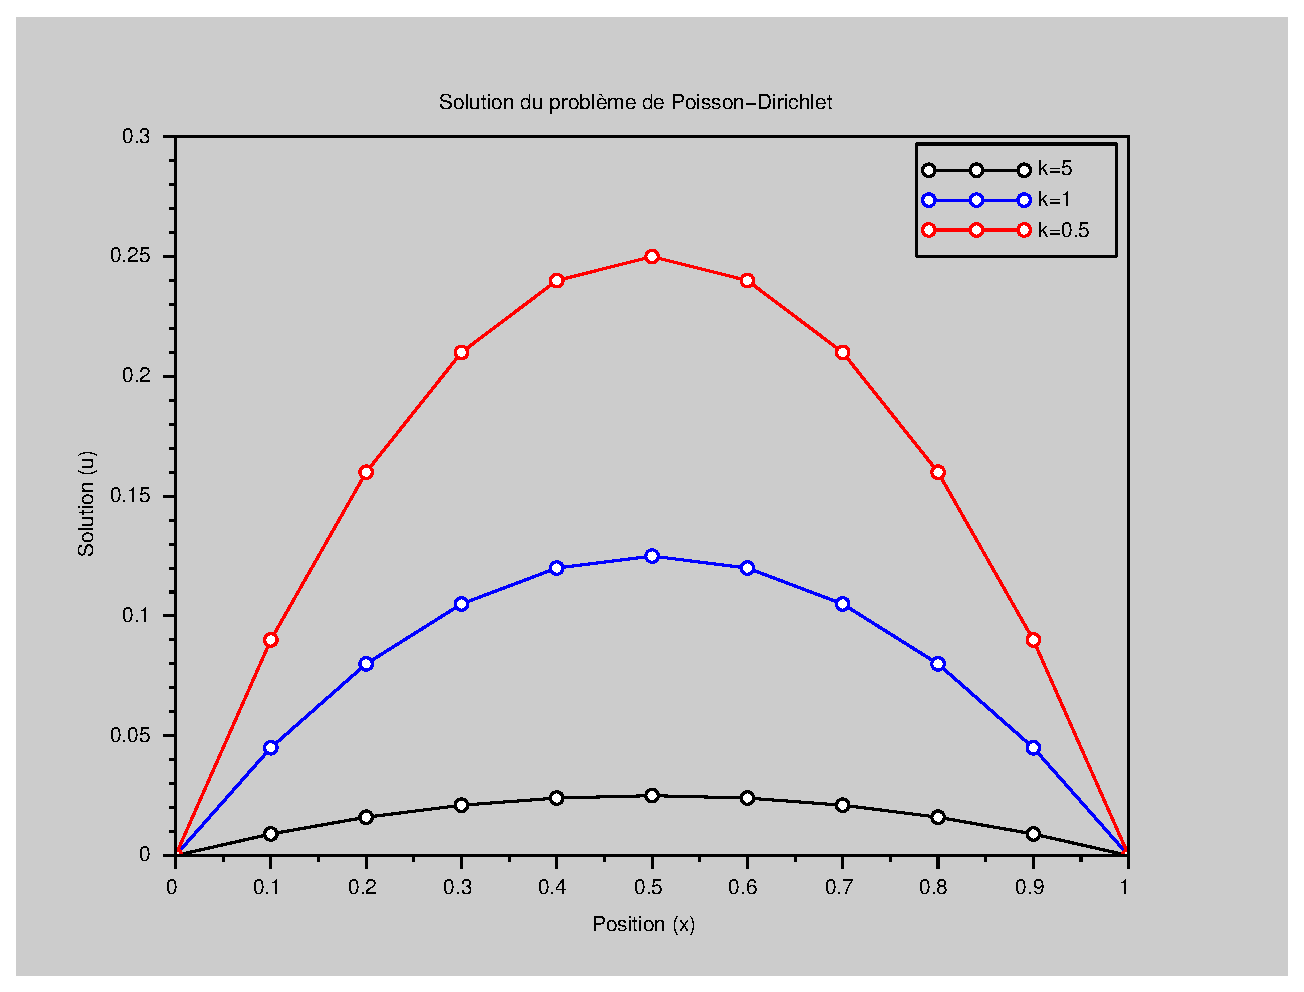
\includegraphics[width = 12cm]{Figures/Poisson_k.eps}
  \caption{Solution de l'\'equation elliptique 1D \eqref{eq:ell_1D}
  pour diff\'erents $k$ (pour $f(x)=1$).}
  \label{fig:ell_k}
\end{figure}


%%%%%%%%%%%%%%%%%%%%%%%%%%%%%%%%%%%%%%%
\subsection{\'Equation de transport}

La deuxi\`eme \'equation que nous \'etudions est l'\'equation de transport
(unidimensionelle).
Elle correspond \`a une quantit\'e qui est transport\'ee \`a vitesse
constante dans une direction.
Cela peut \^etre par exemple un polluant transport\'e par une rivi\`ere.
Dans cette section, nous nous int\'eressons au cas de tas de sable
sur un tapis roulant se d\'epla\c{c}ant \`a vitesse constante $a$.


\begin{figure}
\centering
\begin{tikzpicture}[scale = 0.5]
  %% longueur du tapis roulant
\def\L{15};

%% tapis roulant
\draw (1,0) arc (0:360:1);
\draw (0,1.1) arc (90:270:1.1);
\draw (\L+1.0,0) arc (0:360:1);
\draw (\L,1.1) arc (90:-90:1.1);
\draw (0,1.1) -- (\L,1.1);
\draw (0,-1.1) -- (\L,-1.1);

%% tas de sables (pointilles)
\draw[dashed] (1,1.1) -- (5,3.5) -- (10,2.3) -- (15,5.5);

%% distance parcourue
\def\a{3}

%% tas de sables (trait continu)
\draw (1+\a,1.1) -- (5+\a,3.5) -- (10+\a,2.3) -- (15+\a,5.5);

%% vecteur a
\draw[->] (5,3.9) -- (5+\a,3.9);
\draw (5+\a/2,4.5) node{$a$};

%% hauteur u
\draw[<->] (14,1.2) -- (14,2.8);
\draw (15.3,2.0) node{$u(t,x)$};

%% axe des abscisses
\draw[->] (-1.5,0.0) -- (19.0,0.0);
\draw (19.0,-1.0) node{$x$};

\end{tikzpicture}
\caption{Des tas de sable transport\'es sur un tapis roulant.
  La ligne discontinue repr\'esente les tas en $t=0s$ et la ligne
  continue en $t=1s$.}
\label{fig:transport}
\end{figure}

Sur la figure \ref{fig:transport}, nous repr\'esentons des tas de sables
qui se d\'eplacent \`a vitesse constante $a$ vers la droite.
On note $u(t,x)$ la hauteur du sable en $x$ \`a l'instant $t$.

Si l'on consid\`ere un temps infinit\'esimal $\delta t$,
le sable aura avanc\'e d'une distance $\delta x = a \delta t$.
La hauteur en $(t+\delta t , x + \delta x)$ sera la m\^eme qu'elle
\'etait en $(t,x)$, on traduit cela par $u(t+\delta t, x + a \delta t) = u(t,x)$.
On obtient ainsi l'\'equation
\begin{align}
  \dfrac{\partial u}{\partial t} + a \dfrac{\partial u}{\partial x} = 0 .
\end{align}
Ici, $a$ correspond \`a la vitesse du transport.
Si $a$ est positif, le sable bouge vers la droite; si $a$ est n\'egatif,
le sable bouge vers la gauche; plus $a$ est grand en valeur absolue, 
plus le mouvement est rapide.


\begin{remark}
  En se r\'ef\'erant \`a la d\'efinition, cette \'equation n'est ni elliptique, 
  ni parabolique, ni hyperbolique. Cependant, le comportement des solutions de 
  cette \'equation est proche d'un comportement hyperbolique.
  Notons par ailleurs que l'\'equation \eqref{eq:EDP_geom} associ\'ee
  \`a l'\'equation de transport est une droite et les hyperboles ont des droites
  comme asymptotes.
\end{remark}

Pour finir la pr\'esentation de l'\'equation de transport,
nous donnons des r\'esultats num\'eriques pour diff\'erentes
valeurs de la vitesse de transport $a$ (voir figure \ref{fig:transport_a}).
Ces r\'esultats illustrent bien le fait $a$ est la vitesse \`a laquelle
la solution se d\'eplace.


\begin{figure}[h]
  \centering
  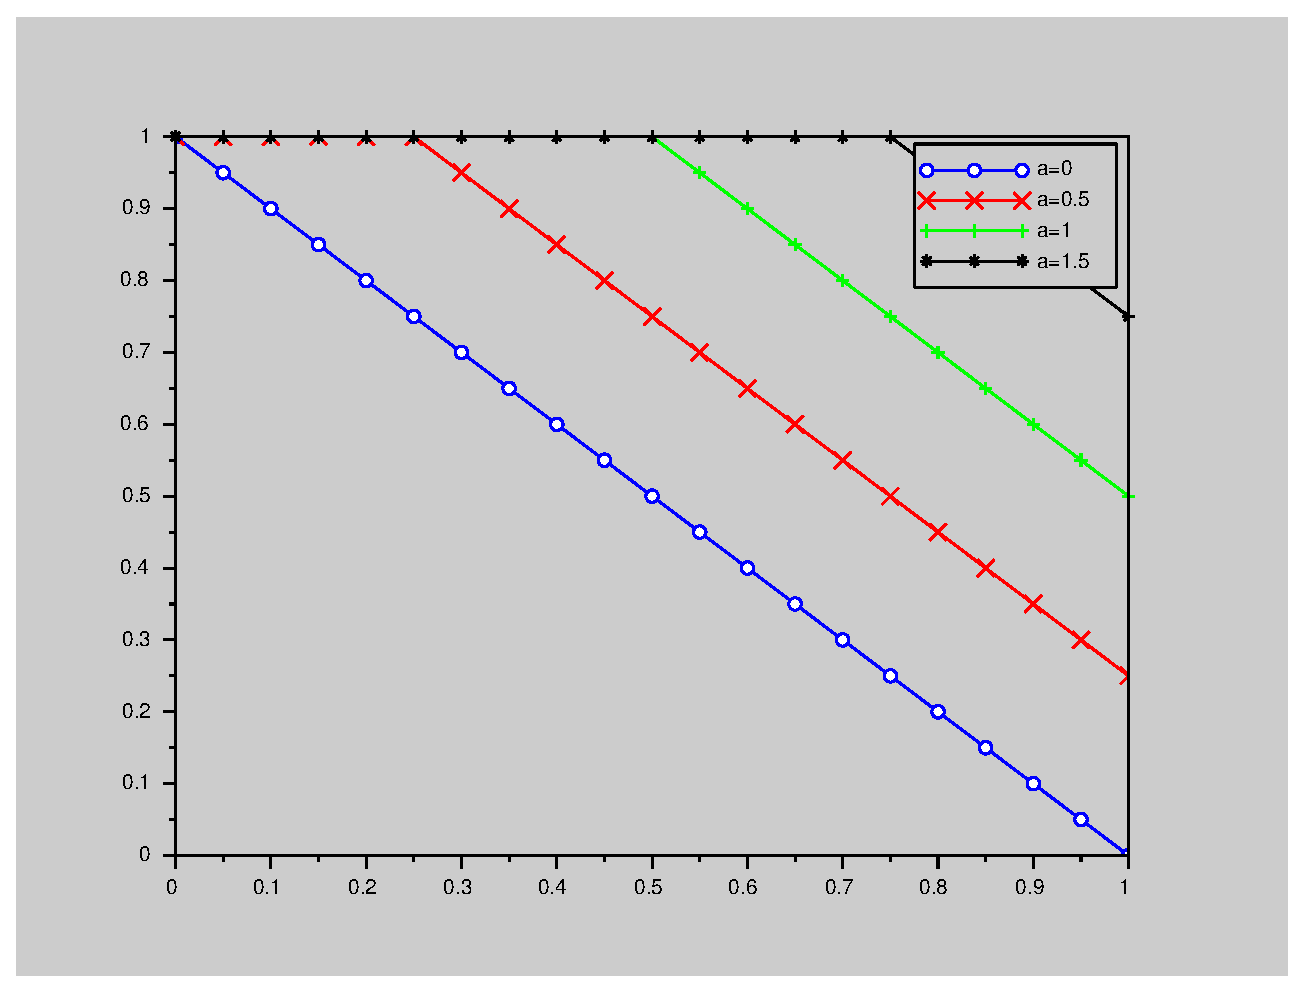
\includegraphics[width = 12cm]{Figures/transport_Dir_a.eps}
  \caption{Solution de l'\'equation de transport \`a $t=0.5$
  pour diff\'erents $a$. La donn\'ee initiale correspond \`a 
  la solution pour $a = 0$.}
  \label{fig:transport_a}
\end{figure}


%%%%%%%%%%%%%%%%%%%%%%%%%%%%%%%%%%%%%%%
\subsection{\'Equation de la chaleur}

On se place dans le cadre du premier probl\`eme que nous avons \'evoqu\'e dans
la section \ref{subsec:elliptique} (voir figure \ref{fig:flux}). 
Pour plus de simplicit\'e, nous consid\'erons que nous sommes dans le cas
de la conduction thermique (bien que comme nous l'avons vu pr\'ec\'edemment
d'autres probl\`emes comme le mouvement d'une population ou de mol\'ecules
peuvent \^etre consid\'er\'es).
La diff\'erence avec ce qui a \'et\'e fait dans la section \ref{subsec:elliptique}
est qu'ici les flux de chaleur ne sont pas n\'ecessairement \`a l'\'equilibre.
On permet donc \`a la temp\'erature de changer au cours du temps.

Nous allons maintenant refaire le raisonnement de la section \ref{subsec:elliptique}
avec cette fois-ci une temp\'erature $u(t,x)$ qui d\'epend du temps.
Si l'on consid\`ere la partie droite de la figure \ref{fig:flux}, l'accumulation
d'\'energie en $(t,x)$ est due au fait que les flux ne sont pas \'equilibr\'es
("ce qui entre n'est pas \'egal \`a ce qui sort").
Ainsi, s'il y a plus d'\'energie qui entre dans le domaine infinit\'esimal
qu'il n'y en a qui en sort,
alors la temp\'erature augmente.
Nous traduisons cela par l'\'equation
$c (x) \delta x \dfrac{\partial u}{\partial t}(t,x) = f(t,x) \delta x 
  + q(t,x) - q(t,x + \delta x)$, ce qui donne
\begin{align}
  \label{eq:flux_t}
  c (x) \dfrac{\partial u}{\partial t}(t,x) = f(t,x) - \dfrac{\partial q}{\partial x} (t,x) .
\end{align}
o\`u $c(x)$ est la capacit\'e thermique lin\'eique du mat\'eriau,
$q(t,x)$ et $f(t,x)$ sont respectivement le flux de chaleur 
et la source de chaleur en $(t,x)$.
Comme pr\'ec\'edemment, le flux de chaleur est proportionnel au gradient 
de temp\'erature (voir \eqref{eq:def_flux}).
Pour simplifier la pr\'esentation, nous consid\'erons que la capacit\'e
thermique $c$ et la conduction thermique $k$ sont des constantes 
(qui ne d\'ependent ni du temps, ni de l'espace).
En combinant les \'equations \eqref{eq:def_flux} et \eqref{eq:flux_t},
on obtient l'\'equation de la chaleur
\begin{align}
  \label{eq:chaleur}
  \dfrac{\partial u}{\partial t} - \nu \dfrac{\partial^2 u}{\partial x^2} = \widetilde{f} ,
\end{align}
o\`u $\nu = k/c > 0$ est la diffusion thermique.


% De mani\`ere similaire \`a ce qui a \'et\'e expliqu\'e dans la section \ref{subsec:elliptique},
% cette l'\'equation de la chaleur, en plus de repr\'esenter l'\'evolution de la temp\'erature
% dans un milieu peut aussi repr\'esenter l'\'evolution de la densit\'e d'une population
% ou encore l'\'evolution d'une concentration chimique d'une esp\`ece au sein d'un diluant.

Les conditions aux limites classiques sont les m\^emes que celles \'evoqu\'ees pour le probl\`eme
stationnaire (voir tableau \ref{tab:pb_ell}).


\begin{figure}[h]
  \centering
  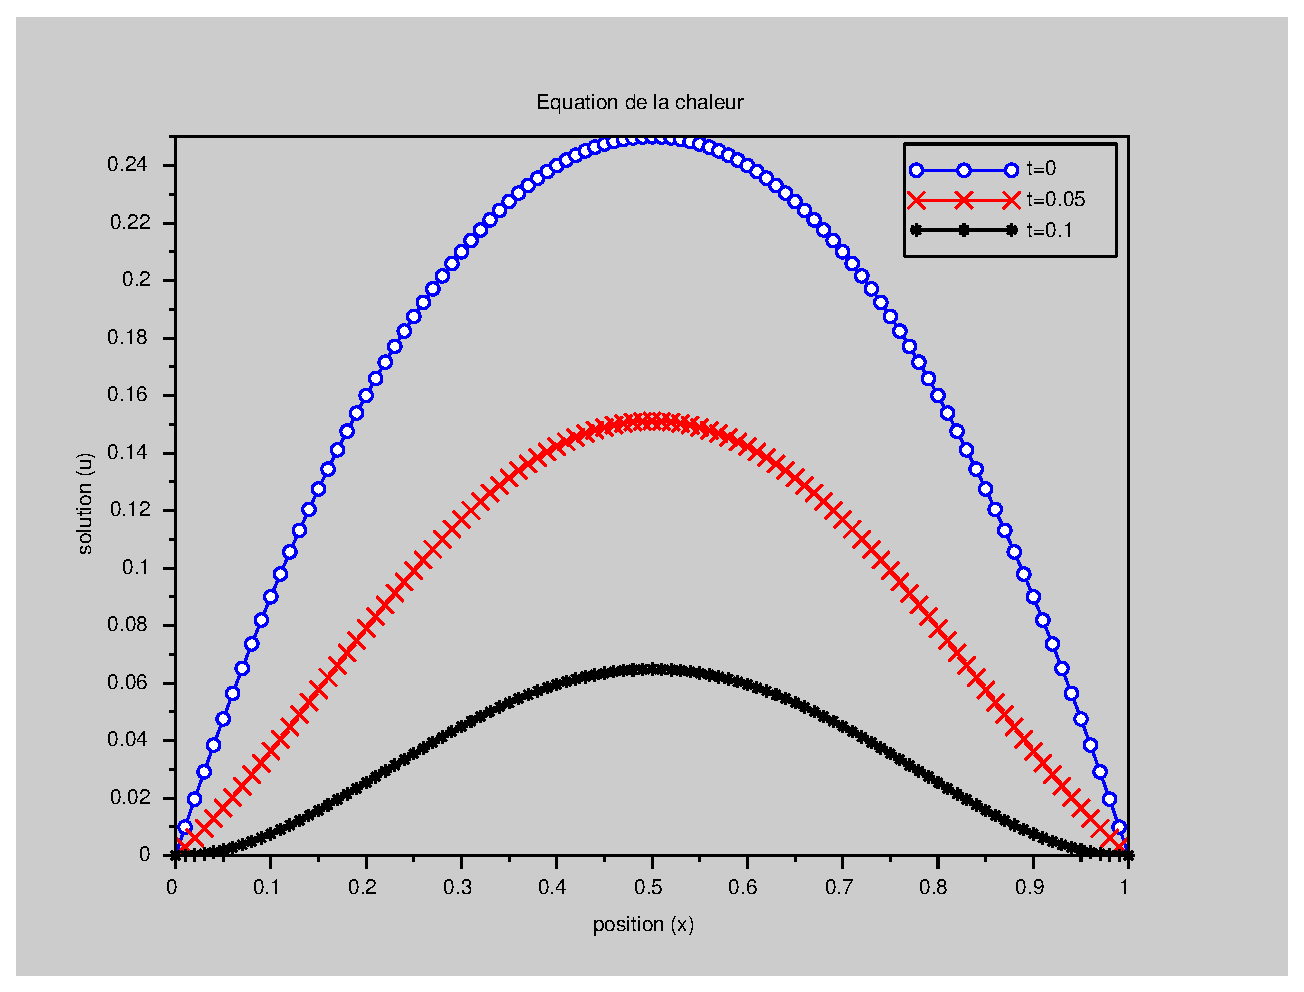
\includegraphics[width = 5.2cm]{Figures/chaleur_nu0_5.eps}
  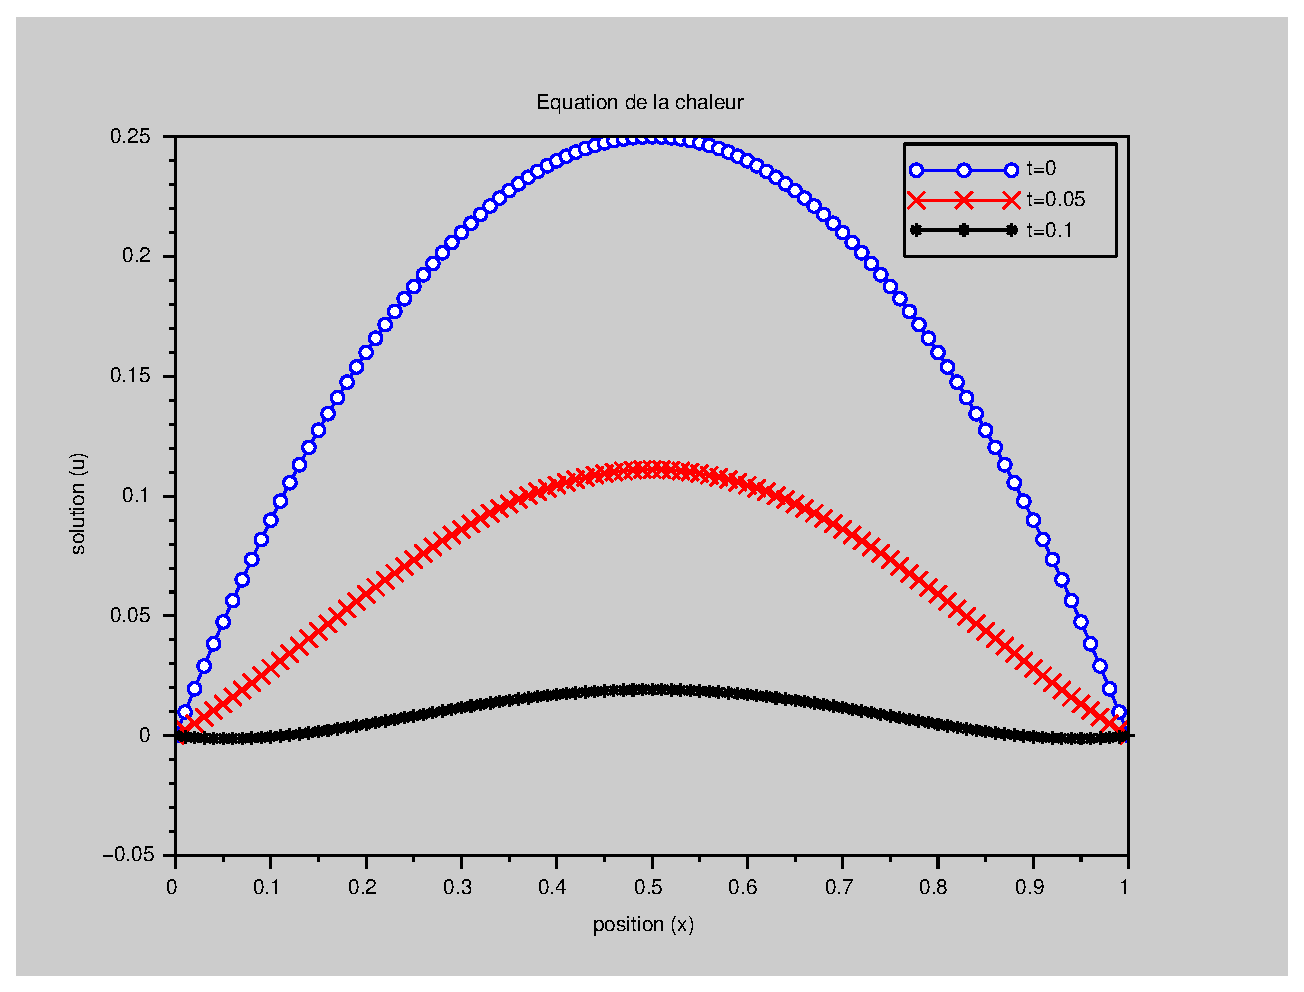
\includegraphics[width = 5.2cm]{Figures/chaleur_nu1.eps}
  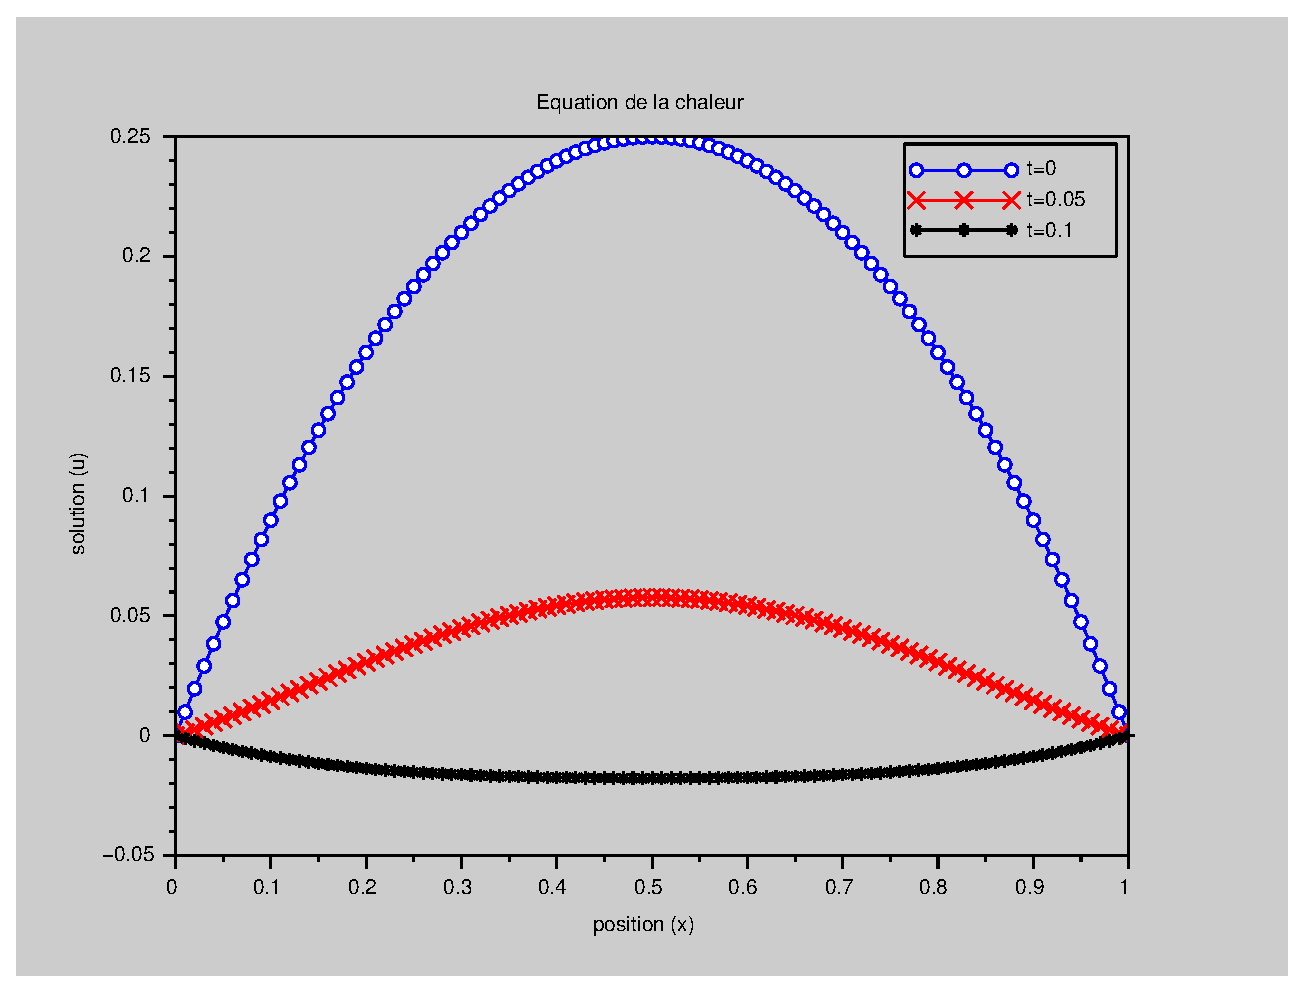
\includegraphics[width = 5.2cm]{Figures/chaleur_nu2.eps}
  \caption{Solution de l'\'equation de la chaleur
  pour $f(x) = -1$. Gauche: $\nu = 0.5$.
  Milieu: $\nu = 1$. Droite: $\nu = 2$.
  Les courbes repr\'esentent la solution \`a $t=0$ (bleu), $t=0.05$ (rouge) et $t=0.1$ (noir).}
  \label{fig:chaleur_nu}
\end{figure}


Nous illustrons sur la figure \ref{fig:chaleur_nu} l'influence du param\`etre $\nu$.
Plus $\nu$ est grand, plus la chaleur va se diffuser rapidement et plus 
la courbe va s'applatir rapidement.

\begin{exercise}
  Prouver que l'\'equation \eqref{eq:chaleur} est une \'equation parabolique.
\end{exercise}


%%%%%%%%%%%%%%%%%%%%%%%%%%%%%%%%%%%%%%%
\subsection{\'Equation des ondes}

L'\'equation des ondes peut \^etre obtenue en consid\'erant un mod\`ele m\'ecanique
comme celui de la figure \ref{fig:barre} o\`u cette fois-ci les forces ne
sont pas n\'ecessairement \`a l'\'equilibre et o\`u les d\'eplacements
$u(t,x)$ peuvent varier au cours du temps.

Le principe fondamental de la dynamique appliqu\'e \`a une tranche de mati\`ere
de longueur $\delta x$ nous dit que l'acc\'el\'eration de la position de cette tranche
($x+u(t,x)$) multipli\'ee par sa masse est \'egale \`a la somme des forces qui
agissent sur elle.
Ainsi, $\rho(x) \delta x \dfrac{\partial^2 u}{\partial t^2} = 
f(t,x) \delta x + q(t,x) - q(t, x + \delta x)$, ce qui nous donne l'\'equation
\begin{align}
  \label{eq:barre_t}
  \rho(x) \dfrac{\partial^2 u}{\partial t^2}(t,x) + \dfrac{\partial q}{\partial x}(t,x) = f(t,x) ,
\end{align}
o\`u $\rho(x)$ correspond \`a la masse de la barre par unit\'e de longueur.
Plus $\rho$ est grand, plus la barre a d'inertie et plus elle acc\'el\`ere lentement.
Notons \`a ce stade qu'il y a, dans cette \'equation, une d\'eriv\'ee seconde en temps
\`a la place de la d\'eriv\'ee premi\`ere qu'il y avait dans \eqref{eq:flux_t}.

La force de compression \`a travers la barre est donn\'ee par la loi d'\'elasticit\'e
\eqref{eq:def_flux}.
Pour simplifier la pr\'esentation, on consid\`ere que la raideur $k$ et la masse
lin\'eique $\rho$ sont constantes (ne d\'ependent ni de $t$ ni de $x$).
En combinant \eqref{eq:def_flux} et \eqref{eq:barre_t} on obtient l'\'equation des ondes
\begin{align}
  \label{eq:ondes}
  \dfrac{\partial^2 u}{\partial t^2} - c^2 \dfrac{\partial^2 u}{\partial x^2} = \widetilde{f} ,
\end{align}
o\`u $c>0$ d\'efini par $c^2 = k/\rho$ correspond \`a la vitesse de propagation
des ondes dans ce milieu.



\begin{figure}[h]
  \centering
  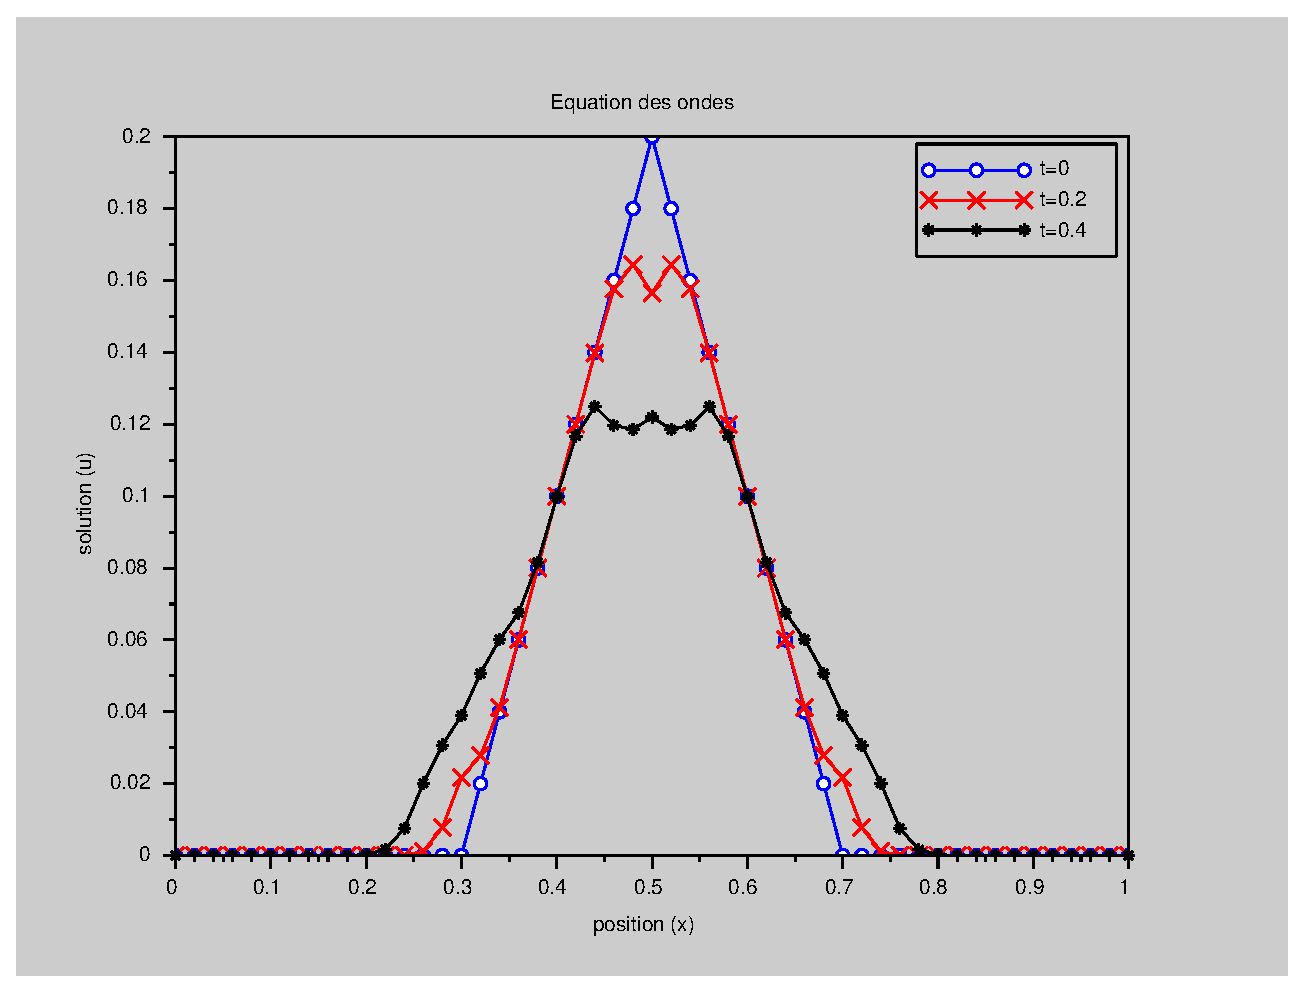
\includegraphics[width = 5.2cm]{Figures/ondes_c0_2.eps}
  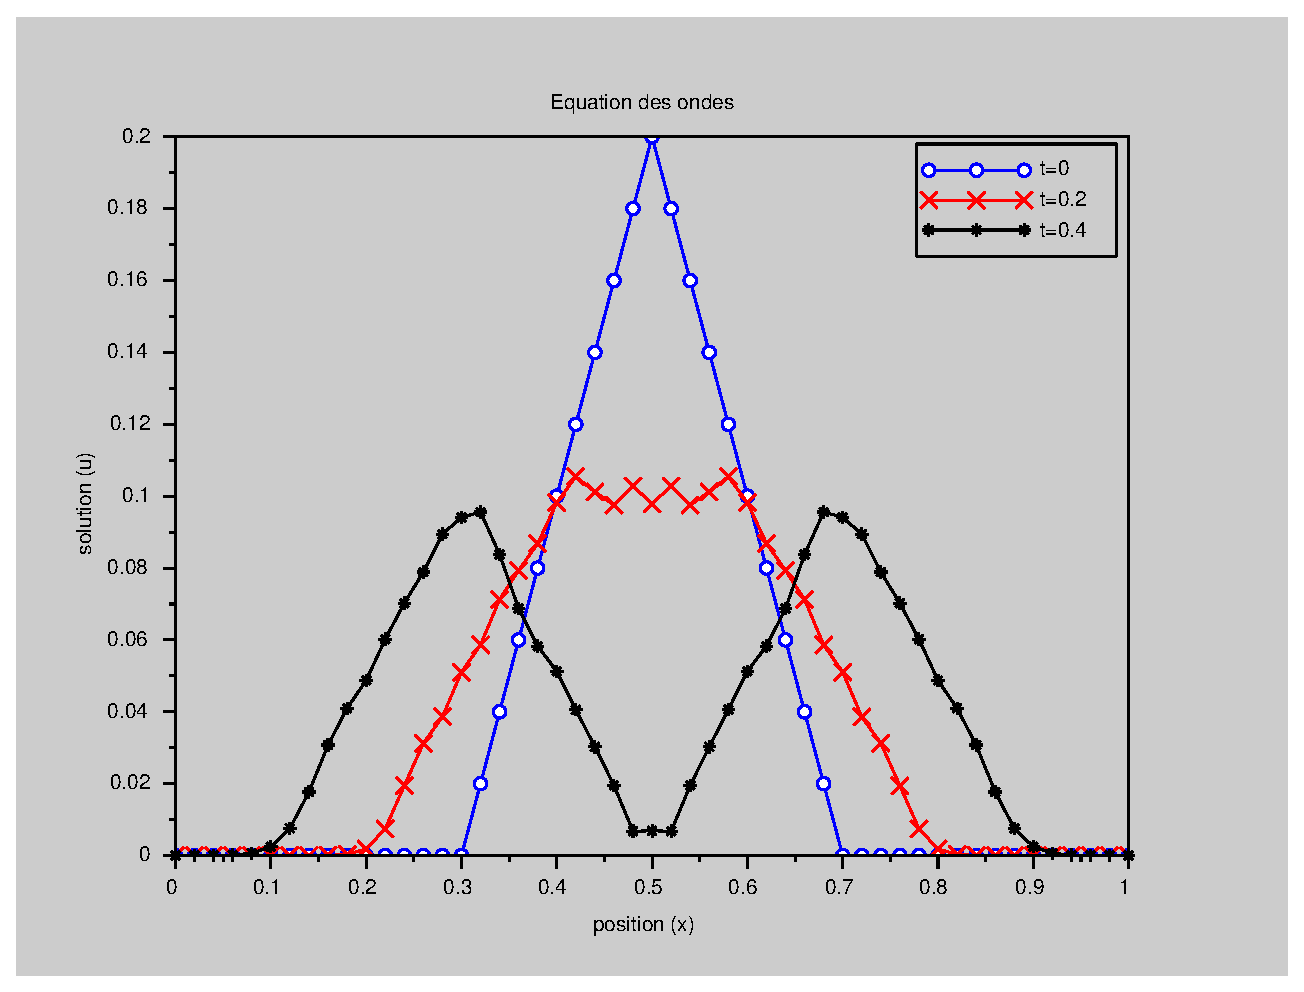
\includegraphics[width = 5.2cm]{Figures/ondes_c0_5.eps}
  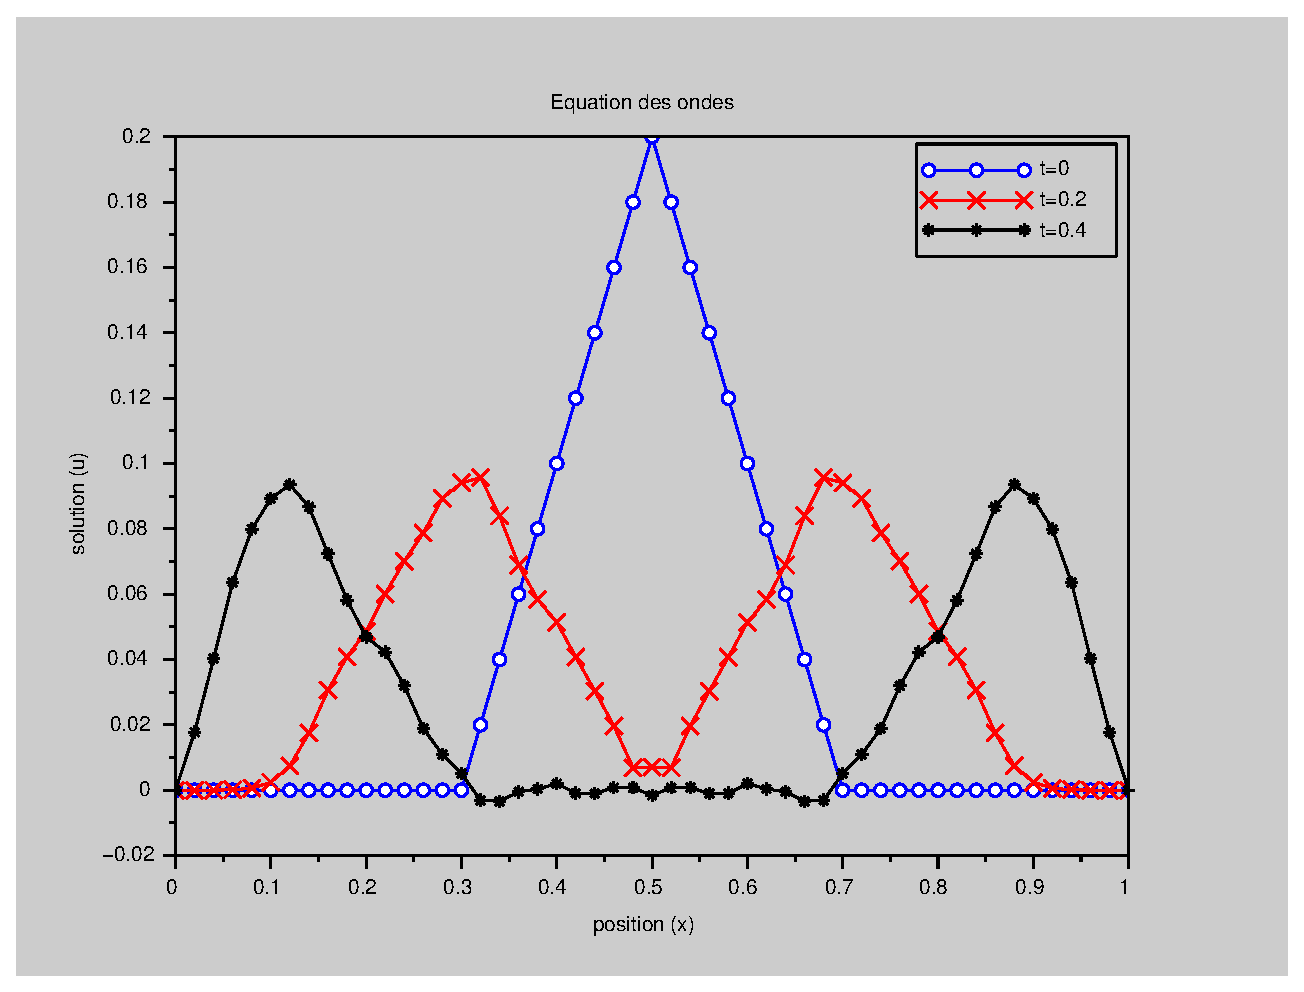
\includegraphics[width = 5.2cm]{Figures/ondes_c1.eps}
  \caption{Solution de l'\'equation des ondes pour $f=0$ et $v_0 = 0$.
  Gauche: $c = 0.2$. Milieu: $c=0.5$. Droite: $c=1$.
  Les courbes repr\'esentent la solution \`a $t=0$ (bleu),
  $t=0.2$ (rouge) et $t=0.4$ (noir).}
  \label{fig:ondes_c}
\end{figure}


On illustre l'influence de $c$ sur la figure \ref{fig:ondes_c}.
Nous voyons que nous avons une propagation de l'information 
dans les deux directions (les $x$ positifs et les $x$ n\'egatifs).
Plus $c$ est grand, plus l'information se propage rapidement.
Notons \'egalement que la solution pour $c=0.5$ et $t=0.4$
correspond \`a la solution pour $c=1.0$ et $t=0.2$.
On voit donc bien que $c$ correspond \`a une vitesse de propagation
de l'onde.


Nous avons \'evoqu\'e le fait que l'\'equation des ondes
pouvait repr\'esenter le d\'eplacement d'une barre en compression.
On peut aussi mod\'eliser des probl\`emes 
comme la propagation du d\'eplacement d'une corde ou
la propagation d'une onde \'electromagn\'etique
(on ne s'\'etendra pas davantage sur le sujet).


Rappelons enfin que les conditions aux limites classiques sont 
les m\^emes que celles du cas stationnaire
(voir tableau \ref{tab:pb_ell}).

\begin{exercise}
  Prouver que l'\'equation \eqref{eq:ondes} est hyperbolique.
\end{exercise}

%%%%%%%%%%%%%%%%%%%%%%%%%%%%%%%%%%%%%%%%%%%%%%%%%%%%%%%%%%%%%%%%%%%%%%%%%%%%%%%%%%%%
\section{\'Equation de Poisson}

On consid\`ere $\Omega$ un ouvert born\'e de $\R^d$ avec $d \in \{1,2,3\}$.
Nous simplifions le cadre \'evoqu\'e pr\'ec\'edemment
en consid\'erant $k=1$.
On s'int\'eresse donc au probl\`eme
\begin{equation}
  \label{eq:ell_Dir}
  \text{Trouver $u \in C^2(\Omega)$ telle que  }
  \left\{
    \begin{array}{l l}
      - \Delta u = f &\dans \Omega ,
      \\
      u = 0 &\sur \partial \Omega .
    \end{array}
  \right.
\end{equation}

%%%%%%%%%%%%%%%%%%%%%%%%%%%%%%%%%%%%%%%
\subsection{Propri\'et\'es g\'en\'erales de l'\'equation}

\begin{theorem}[Existence et unicit\'e de la solution]
  \label{thm:ell_existence}
  Si $f \in C^0(\Omega)$, alors il existe une unique solution
  $u \in C^2(\Omega)$ au probl\`eme \eqref{eq:ell_Dir}.
  De plus, pour $\ell \in \N$, si $f \in C^{\ell}(\Omega)$, alors
  $u \in C^{\ell+2}(\Omega)$.
\end{theorem}

Dans ce th\'eor\`eme nous voyons l'effet r\'egularisant de l'\'equation de Poisson:
si le terme source est de classe $C^{\ell}$ alors la solution du probl\`eme
est de classe $C^{\ell + 2}$.
Les outils utilis\'es pour \'etablir cette preuve sont pr\'esent\'es
dans la section \ref{subsec:LM}.

\begin{proposition}[Principe du maximum]
  On se place dans le cadre du th\'eor\`eme \ref{thm:ell_existence}.
  Si $f \leq 0$, alors $u \leq 0$. En particulier,
  $\max_{x\in \Omega} u(x) = \max_{x\in \partial \Omega} u(x) = 0$.
  Si de plus il existe $m\in \Omega$ tel que $u(m) = 0$,
  alors $\forall x \in \Omega$, $u(x) = 0$ 
  (principe du maximum fort).
\end{proposition}

%% reference vers un livre ??


\begin{definition}[Fonctions harmoniques]
  Si $u \in C^2(\Omega)$ et $- \Delta u = 0$ dans $\Omega$,
  on dit que $u$ est une fonction harmonique.
\end{definition}

Il existe des liens entre fonctions harmoniques et fonctions holomorphes.
En effet, si $\varphi$ est une fonction holomorphe,
alors $\Re(\varphi)$ et $\Im(\varphi)$ (parties r\'eelle et imaginaire)
sont des fonctions harmoniques.


D'autres conditions aux limites peuvent \^etre consid\'er\'ees.
Nous pouvons par exemple consid\'erer des conditions de Dirichlet 
non homog\`enes.
\begin{equation*}
  \text{Trouver $u \in C^2(\Omega)$ telle que  }
  \left\{
    \begin{array}{l l}
      - \Delta u = f &\dans \Omega ,
      \\
      u = g &\sur \partial \Omega ,
    \end{array}
  \right.
\end{equation*}
o\`u $g \in C^2(\partial \Omega)$ est une donn\'ee du probl\`eme.
Pour r\'esoudre ce probl\`eme, on consid\`ere un rel\`evement de $g$,
c'est-\`a-dire une fonction $\tilde{g} \in C^2(\Omega)$ telle que
$\tilde{g} = g$ sur $\partial \Omega$,
et on cherche la solution $u$ sous la forme
$u = \tilde{u} + \tilde{g}$.
La fonction $\tilde{u}$ est alors solution du probl\`eme
homog\`ene
\begin{equation*}
  \text{Trouver $\tilde{u} \in C^2(\Omega)$ telle que  }
  \left\{
    \begin{array}{l l}
      - \Delta \tilde{u} = f + \Delta \tilde{g} &\dans \Omega ,
      \\
      \tilde{u} = 0 &\sur \partial \Omega .
    \end{array}
  \right.
\end{equation*}
Moyennant l'existence du rel\`evement $\tilde{g}$
r\'esoudre le probl\`eme non homog\`ene revient \`a 
r\'esoudre un probl\`eme homog\`ene \'equivalent.


Nous pouvons \'egalement consid\'erer des conditions
de Neumann. Le probl\`eme de Poisson devient alors
\begin{align}
  \label{eq:ell_Neu}
  \text{Trouver $u \in C^2(\Omega)$ telle que  }
  \left\{
    \begin{array}{l l}
      - \Delta u = f &\dans \Omega ,
      \\
      \GRAD u \SCAL n = 0 &\sur \partial \Omega ,
      \\
      \int_{\Omega} u \deriv x = 0 ,
    \end{array}
  \right.
\end{align}
o\`u $n$ d\'esigne la normale sortante au domaine.


Dans le probl\`eme \eqref{eq:ell_Neu}, 
la condition $\int_{\Omega} u \deriv x = 0$ a \'et\'e ajout\'ee
pour garantir l'unicit\'e de la solution. 
En effet, si on enlevait cette condition, pour $u$ solution
de \eqref{eq:ell_Neu}, $u+c$ serait aussi solution pour tout $c\in \R$.
Des alternatives existent \`a la condition 
$\int_{\Omega} u \deriv x = 0$,
l'essentiel est d'\'eliminer l'infinit\'e de solutions g\'en\'er\'ees en
ajoutant $c\in\R$.

Terminons cette section en relevant le fait que l'existence d'une solution
au probl\`eme \eqref{eq:ell_Neu} requiert la condition
$\int_{\Omega} f \deriv x = 0$.

\begin{exercise}
  Prouver que s'il existe une solution $u$ au probl\`eme \eqref{eq:ell_Neu},
  alors $f$ v\'erifie $\int_{\Omega} f \deriv x = 0$.
\end{exercise}

%%%%%%%%%%%%%%%%%%%%%%%%%%%%%%%%%%%%%%%
\subsection{Formulation variationnelle, th\'eor\`eme de Lax--Milgram}
\label{subsec:LM}

Le but de cette section est de pr\'esenter les outils utilis\'es pour prouver 
le th\'eor\`eme \ref{thm:ell_existence}.
Nous utilisons notamment le th\'eor\`eme de Lax--Milgram.

\begin{theorem}[Lax--Milgram]
  \label{thm:Lax-Milgram}
  On fait les hypoth\`eses suivantes.
  \begin{itemize}
  \item Soit $V$ un espace de Hilbert.
  \item Soit $\ell$ une forme lin\'eaire continue sur $V$
    (il existe $C_{\ell} > 0$ tel que $\forall v \in V, |\ell(v)| \leq C_{\ell} \| v \|_{V}$).
  \item Soit $a$ une forme bilin\'eaire continue sur $V$
    (il existe $C_{a} > 0$ tel que $\forall v,w \in V, |a(v,w)| \leq C_{a} \| v \|_{V} \| w \|_{V}$).
  \item On suppose de plus que $a$ est coercive:
    il existe $\alpha > 0$ tel que $\forall v \in V, a(v,v) \geq \alpha \| v \|_{V}^2$.
  \end{itemize}
  Sous ces hypoth\`eses le probl\`eme suivant est bien pos\'e:
  \begin{equation}
    \label{eq:Lax-Milgram}
    \text{Trouver $u \in V$, tel que $\forall v \in V$, } a(u,v) = \ell(v) .
  \end{equation}
  Ceci signifie que le probl\`eme \eqref{eq:Lax-Milgram} admet une unique solution $u \in V$
  et que celle-ci v\'erifie $\| u \|_{V} \leq \dfrac{C_{\ell}}{\alpha}$.
\end{theorem}

%% ref vers un livre 

Pour utiliser ce th\'eor\`eme, \'ecrivons le probl\`eme \eqref{eq:ell_Dir} sous
sa forme variationnelle.
On introduit l'espace de Sobolev
\begin{align}
  H_0^1(\Omega) := \{ v \in L^2(\Omega) \st \GRAD v \in L^2(\Omega) 
  \text{ et } v_{| \partial \Omega} = 0 \sur \partial \Omega \} ,
\end{align}
o\`u $\GRAD v$ est d\'efini au sens des distributions et $v_{|\partial \Omega}$
est la trace de $v$ sur le bord du domaine.


Si $u$ est une solution de \eqref{eq:ell_Dir}, alors pour tout $v \in H^1_0(\Omega)$
on peut \'ecrire
\begin{align*}
  \int_{\Omega} - \Delta u v \deriv x = \int_{\Omega} f v \deriv x .
\end{align*}
En int\'egrant par parties on obtient 
\begin{align*}
  \int_{\Omega} \GRAD u \SCAL \GRAD v \deriv x 
  - \int_{\partial \Omega} (\GRAD u \SCAL n) v \deriv s = \int_{\Omega} f v \deriv x .
\end{align*}
Puisque $v_{|\partial \Omega} = 0$, le deuxi\`eme terme de cette expression est nul.
Nous avons donc \'etabli la proposition suivante.
\begin{proposition}
  Toute solution du probl\`eme \eqref{eq:ell_Dir} est solution du probl\`eme 
  \begin{equation}
    \label{eq:LM2}
    \text{Trouver $u \in H_0^1(\Omega)$, tel que $\forall v \in H_0^1(\Omega)$, } 
    \int_{\Omega} \GRAD v \SCAL \GRAD v \deriv x = \int_{\Omega} f v \deriv x .
  \end{equation}
\end{proposition}

\begin{proposition}
  Le probl\`eme \eqref{eq:LM2} est bien pos\'e.
\end{proposition}
\begin{proof}
  Le probl\`eme \eqref{eq:LM2} correspond au probl\`eme \eqref{eq:Lax-Milgram}
  avec $V = H_0^1(\Omega)$, 
  $\forall v, w \in H_0^1(\Omega), a(v,w) = \int_{\Omega} \GRAD v \SCAL \GRAD v \deriv x$
  et $\ell(v) = \int_{\Omega} f v \deriv x$.
  Nous allons montrer que toutes les hypoth\`eses du th\'eor\`eme de Lax--Milgram
  sont v\'erifi\'ees.
  On admet le fait que $H_0^1(\Omega)$ \'equip\'e de la norme 
  $\| v \|_{H^1(\Omega)} := (\int_{\Omega} v^2 + \GRAD v \SCAL \GRAD v \deriv x)^{1/2}$ 
  est un espace de Hilbert (se reporter \`a un cours sur les distributions).
  D'apr\`es l'in\'egalit\'e de Cauchy--Schwarz, on a 
  $|\ell(v)| \leq (\int_{\Omega} f^2 \deriv x)^{1/2} (\int_{\Omega} v^2 \deriv x)^{1/2}
  \leq (\int_{\Omega} f^2 \deriv x)^{1/2} \| v \|_{H^1(\Omega)}$.
  La forme lin\'eaire $\ell$ est donc continue. 
  
  
  De la m\^eme fa\c{c}on, l'in\'egalit\'e de Cauchy--Schwarz permet de prouver
  que la forme bilin\'eaire $a$ est continue.
  Pour finir, nous utilisons l'in\'egalit\'e de Poincar\'e: il existe $c>0$
  tel que $\forall v \in H_0^1(\Omega), 
  \int_{\Omega} v^2 \deriv x \leq c \int_{\Omega} \GRAD v \SCAL \GRAD v \deriv x$.
  Avec cette in\'egalit\'e, on peut prouver que $a$ est coercive.
  Toutes les hypoth\`eses du th\'eor\`eme de Lax--Milgram sont r\'eunies,
  le probl\`eme \eqref{eq:LM2} est donc bien pos\'e.
\end{proof}

\begin{remark}
  Les r\'esultats de cette section prouvent l'unicit\'e de la solution
  de \eqref{eq:ell_Dir}. On a \'egalement prouv\'e l'existence d'une
  solution \`a \eqref{eq:LM2}. Pour prouver le th\'eor\`eme
  \ref{thm:ell_existence}, il faut montrer que si $f \in C^{\ell}(\Omega)$
  alors la solution de \eqref{eq:LM2} est dans $C^{\ell+2}(\Omega)$
  et est solution de \eqref{eq:ell_Dir}. Cependant cette preuve est 
  tr\`es d\'elicate et nous ne la d\'evelopperons pas ici.
\end{remark}


\begin{remark}
  On dit qu'une solution de \eqref{eq:ell_Dir}
  est une solution forte du probl\`eme de Poisson au sens
  o\`u les d\'eriv\'ees sont des d\'eriv\'ees usuelles.
  On dit qu'une solution de \eqref{eq:LM2} est une solution
  faible du probl\`eme de Poisson au sens o\`u les d\'eriv\'ees
  sont des d\'eriv\'ees faibles (au sens des distributions).
  Nous avons montr\'e qu'une solution forte est une solution faible.
  La r\'eciproque est plus d\'elicate et n\'ecessite des hypoth\`eses
  sur la r\'egularit\'e de $f$.
\end{remark}


\begin{exercise}
  On note $H^1 = \{ v \in L^2(\Omega) \st \GRAD u \in L^2(\Omega) \}$
  et $H_{\bullet}^1 = \{ v \in H^1(\Omega) \st \int_{\Omega} v \deriv x = 0 \}$.
  Prouver que toute solution du probl\`eme \eqref{eq:ell_Neu}
  est solution de la formulation variationnelle
  \begin{align}
    \label{eq:LM2_Neu}
    \text{Trouver $u \in H_{\bullet}^1(\Omega)$, tel que $\forall v \in H_{\bullet}^1(\Omega)$, } 
    \int_{\Omega} \GRAD v \SCAL \GRAD v \deriv x = \int_{\Omega} f v \deriv x .
  \end{align}
  Prouver de plus que le probl\`eme \eqref{eq:LM2_Neu} est bien pos\'e.

  Pour cela, on supposera que $H_{\bullet}^1$ \'equip\'e de la norme $\| \cdot \|_{H^1(\Omega)}$
  introduite pr\'ec\'edemment est un espace de Hilbert.
  On pourra \'egalement utiliser l'in\'egalit\'e de Poincar\'e--Wirtinger:
  il existe une constante $C>0$ telle que
  \begin{equation*}
    \forall v \in H^1(\Omega) , \qquad
    \int_{\Omega} \left( v - \dfrac{1}{|\Omega|} \int_{\Omega} v(x') \deriv x' \right)^2
    \deriv x \leq C \int_{\Omega} \GRAD v \SCAL \GRAD v \deriv x .
  \end{equation*}
\end{exercise}
%%%%%%%%%%%%%%%%%%%%%%%%%%%%%%%%%%%%%%%
\subsection{Discr\'etisation par la m\'ethode des diff\'erences finies}
\label{subsec:ell_DF}

Le but de la m\'ethode des diff\'erences finies est d'approcher la solution 
d'une EDO (\'equation aux d\'eriv\'ees ordinaires) ou EDP
(\'equation aux d\'eriv\'ees partielles) par des valeurs cens\'ees repr\'esenter
cette fonction en certains points. Dans toutes les discr\'etisations abord\'ees dans ce cours,
nous ne consid\'ererons que le cas de probl\`emes \`a une dimension en espace
(les probl\`emes instationnaires auront une deuxi\`eme dimension correspondant au temps).

Par exemple, int\'eressons nous au probl\`eme \eqref{eq:ell_Dir} avec $\Omega = (0,1)$.
Notre probl\`eme est donc
\begin{equation}
  \label{eq:ell_1d}
  \left\{
    \begin{array}{l}
      - \dfrac{\!\deriv^2 u}{\!\deriv x^2} = f \dans (0,1) ,
      \\
      u(0) = u(1) = 0 .
    \end{array}
  \right.
\end{equation}

Nous discr\'etisons l'intervalle $(0,1)$ en $M>0$ sous-intervalles.
On d\'efinit donc les points $x_j = j h$ ($0 \leq j \leq M$) o\`u $h = 1/M$.
On a bien $x_0 = 0$ et $x_M = 1$ (voir figure \ref{fig:disc_x}).

\begin{figure}
\centering
\begin{tikzpicture}[scale=1]
\newcounter{it}
% intervalle
\draw (0,0) -- (10,0);
\forloop{it}{0}{\value{it} < 11}{
\draw (\arabic{it},-0.3) -- (\arabic{it},0.3);
}

% temps
\draw (0,-0.6) node {$0$};
\draw (10,-0.6) node {$1$};
\draw (0,0.6) node {$x_0$};
\draw (1,0.6) node {$x_1$};
\draw (10,0.6) node {$x_M$};
\draw (5,0.6) node {$.......$};
\end{tikzpicture} 
\caption{Repr\'esentation de la discr\'etisation de l'intervalle $(0,1)$.}
\label{fig:disc_x}
\end{figure}


\'Etant donn\'e que nous ne disposons que de valeurs en certains points, on ne peut
pas d\'efinir de d\'eriv\'ees au sens usuel. On utilise donc des taux d'accroissement
(rappelons qu'une d\'eriv\'ee est la limite d'un taux d'accroissement).
Par exemple, on peut montrer que 
$\dfrac{\!\deriv^2 u}{\!\deriv x^2}(x) 
= \lim\limits_{h \to 0} \dfrac{u(x+h) - 2 u(x) + u(x-h)}{h^2}$.
Avec les notations introduites pr\'ec\'edemment, cela signifie que,
pour $h$ suffisamment petit, 
\begin{align}
  \label{eq:dx2}
  \dfrac{\!\deriv^2 u}{\!\deriv x^2}(x_j) \simeq \dfrac{u(x_{j+1}) - 2 u(x_j) + u(x_{j-1})}{h^2} .
\end{align}
La m\'ethode des diff\'erences finies consiste donc \`a d\'efinir une suite $(u_j)_{0\leq j \leq M}$
qui reprenne les \'el\'ements du probl\`eme \eqref{eq:ell_1d}. En particulier, il faut remplacer
les d\'eriv\'ees continues par des taux d'accroissment.
Il existe plusieurs fa\c{c}ons de d\'efinir la suite $(u_j)_{0\leq j \leq M}$ et toutes
n'ont pas les m\^emes propri\'et\'es. La propri\'et\'e la plus importante est la convergence:
on veut que $\lim\limits_{M \to +\infty} \max_{0 \leq j \leq M} | u(x_j) - u_j | = 0$.
Nous aborderons plus en d\'etails ces aspects dans la section \ref{subsec:transport_DF}.


Nous proposons maintenant de discr\'etiser le prob\`eme \eqref{eq:ell_1d}
en utilisant \eqref{eq:dx2}.
Nous construisons donc une suite $(u_j)_{0\leq j \leq M}$ v\'erifiant
\begin{equation}
  \label{eq:ell_DF}
  \left\{
    \begin{array}{l}
      \forall 1 \leq j \leq M-1 , - \dfrac{u_{j+1} - 2 u_j + u_{j-1}}{h^2} = f(x_j) ,
      \\
      u_0 = u_M = 0 .
    \end{array}
  \right.
\end{equation}

\begin{proposition}
  La relation \eqref{eq:ell_DF} d\'efinit une unique suite $(u_j)_{0\leq j \leq M}$ dont les valeurs
  peuvent \^etre d\'etermin\'ees en r\'esolvant le syst\`eme lin\'eaire
  $A U = F$, avec 
  \begin{equation}
    \label{eq:mat_DF_Laplacien}
    A = \dfrac{1}{h^2} 
    \begin{pmatrix} 
      2 & -1 & 0 & \cdots
      \\
      -1 & 2 & -1 & 0 & \cdots
      \\
      0 & -1 & 2 & \ddots &
      \\
      \vdots & & \ddots & \ddots & \ddots
      \\
      & & &  \ddots & 2 & -1
      \\
      & &  & & -1 & 2
    \end{pmatrix} , \qquad U = 
    \begin{pmatrix}
      u_1 \\ u_2 \\ \vdots \\ u_{M-1}
    \end{pmatrix} , \qquad F = 
    \begin{pmatrix}
      f(x_1) \\ f(x_2) \\ \vdots \\ f(x_{M-1})
    \end{pmatrix} .
  \end{equation}
\end{proposition}

\begin{proof}
  La relation \eqref{eq:ell_DF} est \'equivalente au syst\`eme lin\'eaire $AU = F$.
  Pour prouver cela, on \'ecrit les \'equations discr\`etes
  \begin{align*}
    &\dfrac{-u_0 + 2 u_1 - u_2}{h^2} = f(x_1) ,
    \\
    &\dfrac{-u_1 + 2 u_2 - u_3}{h^2} = f(x_2) ,
    \\
    &\dfrac{-u_2 + 2 u_3 - u_4}{h^2} = f(x_3) ,
    \\
    & \qquad \qquad \vdots
    \\
    &\dfrac{-u_{M-2} + 2 u_{M-1} - u_M}{h^2} = f(x_{M-1}) .
  \end{align*}
  En prenant en compte $u_0 = u_M = 0$, on obtient bien $AU = F$.
  La r\'eciproque se prouve de mani\`ere similaire.

  Maintenant, le fait que ce syst\`eme admet une unique solution vient de l'inversibilit\'e
  de la matrice $A$ qui est une cons\'equence de la proposition \ref{prop:matSDP}.
\end{proof}


\begin{remark}
  La matrice $A$ doit absolument \^etre connue par c\oe{}ur.
  En effet, ceci est exigible et le jury du concours se plaint dans ses rapports
  que beaucoup trop de candidats ne connaissent pas cette matrice.
\end{remark}

\begin{proposition}
  \label{prop:matSDP}
  La matrice $A$ est sym\'etrique d\'efinie positive.
\end{proposition}


\begin{exercise}
  Prouver la proposition \ref{prop:matSDP}.
\end{exercise}

\begin{proposition}[Convergence]
  \label{prop:ell_conv}
  %% voir Proposition 2.10 du livre de B. Lucquin
  Supposons que la solution $u$ du probl\`eme \eqref{eq:ell_1d} soit 
  dans $C^4(0,1)$.
  Alors il existe $C>0$ tel que pour tout $M \geq 2$, on a
  \begin{align*}
    \max_{0 \leq j \leq M} | u(x_j) - u_j | \leq C h^2 ,
  \end{align*}
  avec $h = 1/M$.
\end{proposition}

\begin{proof}
  \'Etant donn\'e que $u \in C^{4}(0,1)$, on peut utiliser la formule de Taylor--Young
  \begin{align*}
    u(x_{j+1}) = u(x_j) + h u'(x_j) + \dfrac{h^2}{2} u^{(2)}(x_j) + \dfrac{h^3}{6} u^{(3)}(x_j)
    + \dfrac{h^4}{24} u^{(4)}(x_j) + o(h^4) ,
    \\
    u(x_{j-1}) = u(x_j) - h u'(x_j) + \dfrac{h^2}{2} u^{(2)}(x_j) - \dfrac{h^3}{6} u^{(3)}(x_j)
    + \dfrac{h^4}{24} u^{(4)}(x_j) + o(h^4) .
  \end{align*}
  On obtient ainsi
  \begin{align*}
    \dfrac{-u(x_{j+1}) + 2 u(x_j) - u(x_{j-1})}{h^2} = - u^{(2)}(x_j) - \dfrac{h^2}{12} u^{(4)}(x_j)
    + o (h^2) .
  \end{align*}
  On a de plus 
  \begin{align*}
    \dfrac{- u_{j+1} + 2 u_j - u_{j-1}}{h^2} = f(x_j) = - u^{(2)}(x_j) ,
  \end{align*}
  et donc
  \begin{align*}
    \dfrac{-\delta_{j+1} + 2 \delta_j - \delta_{j-1}}{h^2} = \dfrac{h^2}{12} u^{(4)}(x_j) + o(h^2) ,
  \end{align*}
  o\`u $\delta_j = u_j - u(x_j)$.
  En notant $\underline{\delta}$ le vecteur des $\delta_j$,
  on a $\underline{\delta} = A^{-1} \underline{\epsilon}$
  avec $(\underline{\epsilon})_j = O(h^2)$.
  En supposant que $\sup_{X \in \R^{M-1}\backslash \{0\}} \dfrac{\max_{j} |(A^{-1}X)_j|}{\max_j |X_j|}$
  est born\'e quand $h$ tend vers $0$ (on ne le montre pas ici), on obtient le r\'esultat attendu.
\end{proof}

Le r\'esultat pr\'ec\'edent signifie que pour $h$ suffisamment petit
on s'attend \`a ce que l'erreur commise par le sch\'ema num\'erique d\'ecroisse
comme le carr\'e de $h$.
On dit que le sch\'ema est d'ordre $2$, nous \'etudierons plus pr\'ecis\'ement cette notion
plus loin dans le cours.


Cette notion d'ordre de convergence peut-\^etre illustr\'ee en repr\'esentant 
l'erreur commise par le sch\'ema 
$\varepsilon = \max_{0\leq j \leq M} |u(x_j) - u_j|$ en fonction de $h$ 
en utilisant une \'echelle logarithmique
pour les axes des abscisses et des ordonn\'ees.
Par exemple, consid\'erons $f(x) = x^2$, la solution exacte associ\'ee
est $u(x) = \frac{x}{12}(1-x^3)$.
L'erreur du sch\'ema commise sur ce cas test est repr\'esent\'ee
sur la figure \ref{fig:ell_convergence}.
On voit que l'on obtient une droite de pente $2$.
Ceci est en accord avec la proposition \ref{prop:ell_conv} :
si l'erreur est $\varepsilon = C h^2$ alors
$\log(\varepsilon) = 2 \log(h) + \log(C)$.

\begin{figure}[h]
  \centering
  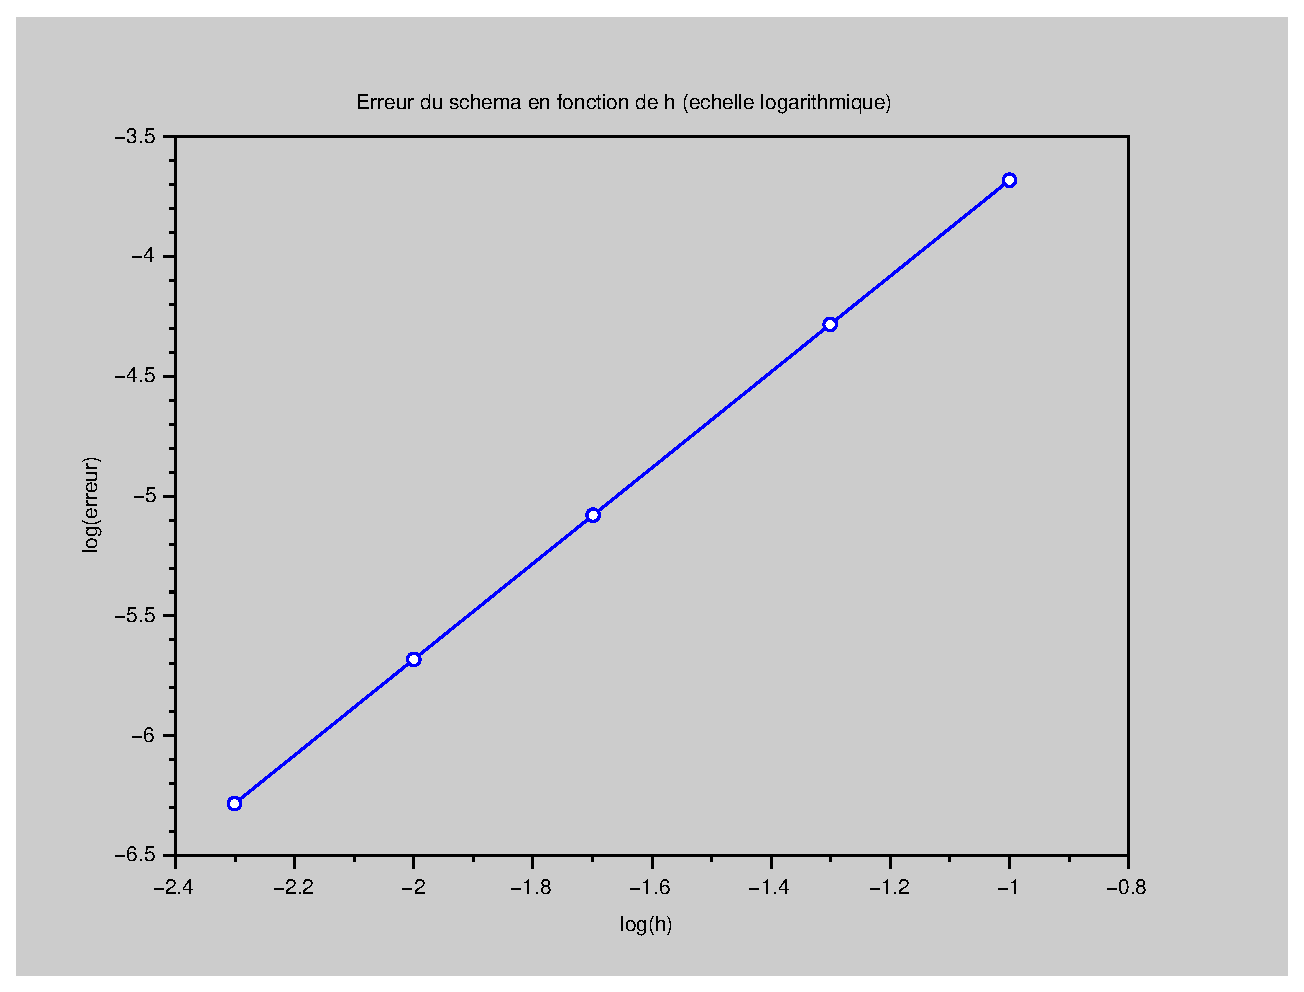
\includegraphics[width = 12cm]{Figures/Poisson_conv.eps}
  \caption{Erreur en fonction de $h$ (\'echelle logarithmique)
    pour $f(x) = x^2$.}
  \label{fig:ell_convergence}
\end{figure}


\begin{exercise}
  Coder le sch\'ema d\'ecrit pr\'ec\'edemment et retrouver les 
  r\'esultats de la figure \ref{fig:ell_convergence}
  (les diff\'erents points ont \'et\'e obtenus pour $M=10$, $20$,
  $50$, $100$ et $200$).
\end{exercise}

\begin{exercise}[Coefficient de raideur]
  On peut d\'ecider d'ajouter un coefficient de raideur $k>0$ constant.
  La nouvelle matrice devient alors $k A$ o\`u $A$ est la matrice 
  pr\'ec\'edente.
  La figure \ref{fig:ell_k} a \'et\'e obtenue pour $f(x) = 1$
  et $M=10$ ($h=1/10$).
  Coder le sch\'ema propos\'e et retrouver les r\'esultats
  de la figure \ref{fig:ell_k}.
  Calculer la solution exacte.
  En d\'eduire l'erreur que commet le sch\'ema.
  Que remarquez-vous?
\end{exercise}


\begin{exercise}[Conditions aux limites de Dirichlet non homog\`enes]
  Adapter le sch\'ema num\'erique pr\'ec\'edent pour approcher
  le probl\`eme
  \begin{align*}
    \left\{
    \begin{array}{l}
      - \dfrac{\!\deriv^2 u}{\!\deriv x^2} = f \dans (0,1) ,
      \\
      u(0) = \alpha ,
      \\
      u(1) = \beta ,
    \end{array}
    \right.
  \end{align*}
  o\`u $\alpha, \beta \in \R$.
  Donner le syst\`eme lin\'eaire \`a r\'esoudre.
\end{exercise}

\begin{exercise}[Condition aux limites de Neumann]
  On consid\`ere le probl\`eme de Poisson avec des conditions aux limites
  de Neumann 
  \begin{align*}
    \left\{
    \begin{array}{l}
      - \dfrac{\!\deriv^2 u}{\!\deriv x^2} = f \dans (0,1) ,
      \\
      u'(0) = u'(1) = 0 ,
      \\
      \int_0^1 u(x) \deriv x = 0 .
    \end{array}
  \right.
  \end{align*}
  \begin{enumerate}
  \item On d\'ecide d'adapter la d\'emarche pr\'ec\'edente en consid\'erant le sch\'ema
    \begin{align*}
      \left\{
      \begin{array}{l}
        \forall 1 \leq j \leq M-1 , - \dfrac{u_{j+1} - 2 u_j + u_{j-1}}{h^2} = f(x_j) ,
        \\
        \dfrac{u_1 - u_0}{h} = \dfrac{u_M - u_{M-1}}{h} = 0.
      \end{array}
      \right.
    \end{align*}
    Calculer la matrice associ\'ee. Montrer qu'elle est positive 
    mais qu'elle n'est pas inversible. Commenter.
  \item On ajoute une condition de moyenne nulle, le sch\'ema devient
    \begin{align*}
      \left\{
      \begin{array}{l}
        \forall 1 \leq j \leq M-1 , - \dfrac{u_{j+1} - 2 u_j + u_{j-1}}{h^2} = f(x_j) ,
        \\
        \dfrac{u_1 - u_0}{h} = \dfrac{u_M - u_{M-1}}{h} = 0 ,
        \\
        \sum\limits_{j=1}^{M-1} u_j = 0 .
      \end{array}
      \right.
    \end{align*}
    On impose la condition de moyenne nulle par un multiplicateur de Lagrange $\alpha \in \R$.
    Le probl\`eme devient $\widetilde{A} \widetilde{U} = \widetilde{F}$ avec
    \begin{align*}
      \widetilde{A} = \dfrac{1}{h^2}
      \begin{pmatrix}
        1 & -1 & & & & h^2
        \\
        -1 & 2 & -1& & & \vdots
        \\
        & \ddots & \ddots & \ddots & & \vdots
        \\
        & & -1 & 2 & -1 & \vdots
        \\
        & &    & -1 & 1 & h^2
        \\
        h^2 & \cdots & \cdots & \cdots &  h^2 & 0
      \end{pmatrix} ,
      \qquad \widetilde{U} = 
      \begin{pmatrix}
        u_1 \\ \vdots \\ u_{M-1} \\ \alpha
      \end{pmatrix} ,
      \qquad \widetilde{F} = 
      \begin{pmatrix}
        f(x_1) \\ \vdots \\ f(x_{M-1}) \\ 0
      \end{pmatrix} .
    \end{align*}
    Montrer que la matrice $\widetilde{A}$ est inversible.
  \item Coder ce sch\'ema et le tester avec $f(x)=1$.
    Que se passe-t-il? Est-ce un comportement normal?
    D'apr\`es vous, que repr\'esente $\alpha$?
  \item Essayons maintenant 
    \begin{align*}
      f(x) = \left\{
      \begin{array}{l}
        1 \quad \text{si} \quad x \in (0,0.5),
        \\
        0 \quad \text{si} \quad x=0.5,
        \\
        -1 \quad \text{si} \quad x \in (0.5,1).
      \end{array}
      \right.
    \end{align*}
    Calculer la solution exacte \`a ce probl\`eme. 
    D\'eterminer num\'eriquement l'ordre de convergence du sch\'ema. 
    Est-ce en contradition avec la proposition \ref{prop:ell_conv}?

  \item On pourra \'egalement reprendre la question pr\'ec\'edente avec
    $f(x) = x-\frac{1}{2}$.
  \end{enumerate}
\end{exercise}

%%%%%%%%%%%%%%%%%%%%%%%%%%%%%%%%%%%%%%%%%%%%%%%%%%%%%%%%%%%%%%%%%%%%%%%%%%%%%%%%%%%%
\section{\'Equation de transport}

Nous \'etudions ici l'\'equation de transport dans un espace \`a une dimension.
Le probl\`eme d\'epend donc d'une variable d'espace $x \in [0,1]$ et d'une variable de temps
$t \in [0,T]$ avec $T>0$.
Nous consid\'erons le probl\`eme
\begin{equation}
  \label{eq:transport}
  \text{Trouver $u \in C^1([0,T] \times [0,1] )$ telle que} \;
  \left\{
    \begin{array}{l}
     \dfrac{\partial u}{\partial t} + a \dfrac{\partial u}{\partial x} = 0 
      \dans (0,T) \times (0,1),
      \\
      \forall t \in (0,T), u(t,0) = \alpha(t) ,
      \\
      \forall x \in (0,1), u(0,x) = u_0(x) ,
    \end{array}
  \right.
\end{equation}
o\`u $a > 0$ correspond \`a la vitesse de transport de l'\'equation,
$\alpha(t)$ est la donn\'ee de Dirichlet \`a gauche
et $u_0$ est la donn\'ee initiale.
Dans l'\'enonc\'e de notre probl\`eme, nous avons not\'e
$C^1([0,T] \times [0,1])$ l'ensemble des fonctions $C^1$
de $[0,T] \times [0,1]$ \`a valeur dans $\R$.
%%%%%%%%%%%%%%%%%%%%%%%%%%%%%%%%%%%%%%%
\subsection{Propri\'et\'es g\'en\'erales}

Le probl\`eme \eqref{eq:transport} admet une unique solution $u$.
Cette solution est obtenue en "d\'epla\c{c}ant" la donn\'ee initiale
vers la droite et en "faisant entrer" la donn\'ee de Dirichlet dans le domaine.
De mani\`ere plus rigoureuse, nous avons le th\'eor\`eme suivant.

\begin{theorem}
  \label{thm:transport_existence}
  Supposons que $a > 0$, $u_0 \in C^1([0,1])$ et $\alpha \in C^1([0,T])$.
  Supposons de plus les conditions de compatibilit\'e $u_0(0) = \alpha(0)$
  et $\alpha'(0) +a u_0'(0)=0$.
  Le probl\`eme \eqref{eq:transport} admet alors une unique solution donn\'ee par
  \begin{align}
    \label{eq:transport_sol}
    u(t,x) = 
    \begin{cases} 
      u_0(x-at) \quad &\text{si} \; x \geq at ,
      \\ 
      \alpha(t-x/a) \quad  &\text{sinon} .
    \end{cases}
  \end{align}
\end{theorem}

\begin{remark}
  On n'a besoin d'une donn\'ee de Dirichlet que d'un seul c\^ot\'e du domaine.
  Puisque l'on a choisi $a > 0$, il faut fixer la donn\'ee de Dirichlet \`a gauche.
  On aurait aussi pu prendre $a < 0$ et utiliser la condition de Dirichlet \`a droite
  $u(t,1) = \alpha(t)$.
\end{remark}


Nous allons maintenant \'evoquer une autre propri\'et\'e int\'eressante de l'\'equation
de transport: la r\'eversibilit\'e de l'\'equation.
Cela signifie qu'en utilisant la solution au temps final et \'eventuellement d'autres donn\'ees
(ici la solution qui sort du domaine \`a droite), on peut reconstituer la solution
en tout temps $t \in [0,T]$.
Il s'agit en fait d'\'etudier un probl\`eme o\`u le temps s'\'ecoule 
"en sens inverse".

\begin{proposition}[R\'eversibilit\'e de l'\'equation de transport]
  \label{prop:transport_rev}
  Soit $u$ une solution du probl\`eme \eqref{eq:transport}.
  Le probl\`eme
  \begin{equation}
    \label{eq:transport_rev}
    \text{Trouver $\tu \in C^1([0,T] \times [0,1] )$ telle que} \;
    \left\{
      \begin{array}{l}
        \dfrac{\partial \tu}{\partial t} - a \dfrac{\partial \tu}{\partial x} = 0 
        \quad \dans (0,T) \times (0,1),
        \\
        \forall t \in (0,T), \qquad \tu(t,1) = u(T-t,1) ,
        \\
        \forall x \in (0,1), \qquad \tu(0,x) = u(T,x) ,
      \end{array}
    \right.
  \end{equation}
  admet une unique solution d\'efinie par
  $\forall t \in [0,T], \forall x \in [0,1]$, 
  $\tu(t,x) = u(T-t,x)$. 
\end{proposition}

Cette propri\'et\'e signifie que l'information est conserv\'ee au cours du temps:
le comportement de l'\'equation ne d\'egrade pas cette information.


%%%%%%%%%%%%%%%%%%%%%%%%%%%%%%%%%%%%%%%
\subsection{M\'ethode des caract\'eristiques}

La m\'ethode des caract\'eristiques consiste \`a montrer que la solution
se conserve sur certaines courbes que l'on appelle trajectoires caract\'eristiques.
Dans le cas monodimensionnel avec $a$ constant, ces courbes sont des droites.
On parlera donc de droites caract\'eristiques.
Cependant, dans le cas o\`u plusieurs dimensions d'espace sont consid\'er\'ees,
ces courbes peuvent \^etre plus complexes (voir la section \ref{subsec:transport_multiD}).

\begin{figure}
\centering
\begin{tikzpicture}[scale = 9]
  %% temps final
\def\T{0.9};

%% repere
\draw[->] (-0.05,0) -- (1.1,0);
\draw (1.1,-0.05) node{$x$};
\draw[->] (0,0.0) -- (0,\T+0.1);
\draw (-0.05,\T+0.1) node{$t$};

%% domaine
\draw[line width=1mm] (0,0) -- (1,0);
\draw (1,-0.05) node{$1$};
\draw (0.0,-0.05) node{$0$};
\draw[line width=1mm] (0,0) -- (0,\T);
\draw (-0.05, \T) node{$T$};
\draw[dashed] (1,0) -- (1,\T);
\draw[dashed] (0,\T) -- (1,\T);

%% courbes caract\'eristiques
\draw (0.75,0) -- (1,0.25);
\draw (0.5,0) -- (1,0.5);
\draw (0.25,0) -- (1,0.75);
\draw (0,0) -- (\T,\T);
\draw (0,0.25) -- (\T-0.25,\T);
\draw (0,0.5) -- (\T-0.5,\T);
\draw (0,0.75) -- (\T-0.75,\T);

%% ronds
\def\r{0.02};
\draw (0.75+\r,0) arc(0:360:\r);
\draw (0.5+\r,0) arc(0:360:\r);
\draw (0.25+\r,0) arc(0:360:\r);
\draw (\r,0) arc(0:360:\r);
\draw (\r,0.25) arc(0:360:\r);
\draw (\r,0.5) arc(0:360:\r);
\draw (\r,0.75) arc(0:360:\r);

\end{tikzpicture}
\caption{Les droites caract\'eristiques de l'\'equation de transport
  ($a=1$ et $T=0.9$).}
\label{fig:D_carac}
\end{figure}

Nous pouvons montrer que dans le cas consid\'er\'e dans cette section,
la solution se conserve sur les droites d'\'equation $x=at+b$ avec 
$a$ la vitesse de transport dans \eqref{eq:transport} et $b \in \R$.
Ces droites sont donc les droites caract\'eristiques de notre probl\`eme,
nous les repr\'esentons sur la figure \ref{fig:D_carac}.
Le r\'esultat de conservation est \'enonc\'e dans la proposition suivante.

\begin{proposition}
  \label{prop:droites_carac}
  Soit $u \in C^1([0,T] \times [0,1])$ v\'erifiant l'\'equation de transport
  \begin{align*}
    \dfrac{\partial u}{\partial t} + a \dfrac{\partial u}{\partial x} = 0 
    \dans (0,T) \times (0,1) ,
  \end{align*}
  avec $a \in \R$.
  Pour tous $t,s \in [0,T]$ et $x \in [0,1]$ tels que
  $t-s \in [0,T]$ et $x-as \in [0,1]$, on a
  \[
    u(t,x) = u(t-s , x-as) .
  \]
\end{proposition}

\begin{exercise}
  Prouver la proposition \ref{prop:droites_carac}.
\end{exercise}


Notons que la proposition \ref{prop:droites_carac} est valable pour tout $a \in \R$
et pour n'importe quelles conditions aux limites. Nous allons maintenant prouver
le th\'eor\`eme \ref{thm:transport_existence}.

\begin{proof}[Preuve du th\'eor\`eme \ref{thm:transport_existence}]
  Commen\c{c}ons par montrer que la fonction $u$ donn\'ee dans \eqref{eq:transport_sol}
  est solution du probl\`eme \eqref{eq:transport}.
  On note $u^+(t,x) = u_0(x-at)$ et $u^-(t,x) = \alpha(t-x/a)$.

  Par construction, les fonctions $u^+$ et $u^-$ sont $C^1$ sur leur domaine de 
  d\'efinition. Nous cherchons \`a les raccorder le long de la droite $x=at$.
  Soit $(t_0,x_0) \in [0,T] \times [0,1]$ qui v\'erifient $x_0 = at_0$.
  On a $\lim_{(t,x) \to (t_0,x_0)} u^+(t,x) = \lim_{s \to 0^+} u_0(s) = u_0(0)
  = \alpha(0) = \lim_{s \to 0^+} \alpha(s) = \lim_{(t,x) \to (t_0,x_0)} u^-(t,x)$.
  La fonction $u$ est donc continue.
  De plus, par un raisonnement similaire, la condition $\alpha'(0) = -au_0'(0)$
  implique que $u$ est dans $C^1([0,T]\times [0,1])$.
  De plus, $u$ v\'erifie la condition initiale $u(0,x) = u_0(x)$ ainsi que la condition
  de Dirichlet $u(t,0) = \alpha(t)$ et elle v\'erifie l'\'equation de transport.
  Il s'agit donc bien d'une solution de \eqref{eq:transport}.

  Supposons maintenant que $v \in C^1([0,T] \times [0,1])$ est solution de
  \eqref{eq:transport}.
  Si $x \leq a t$, on applique la proposition \ref{prop:droites_carac}
  avec $s=x/a$, avec la condition de Dirichlet
  on obtient $u(t,x) = \alpha(t-x/a)$.
  Si $x \geq a t$, on applique la proposition \ref{prop:droites_carac}
  avec $s=t$, avec la condition initiale on obtient $u(t,x) = u_0(x-at)$.
  Nous avons donc prouv\'e l'unicit\'e de la solution.
\end{proof}


Nous voyons donc que la valeur de la solution en $(t,x)$ est \`a aller chercher
sur le bord du domaine espace-temps. C'est-\`a-dire, en fonction de la valeur de 
$t$ et $x$, soit sur la condition initiale, soit sur la donn\'ee de Dirichlet
(l'endroit o\`u r\'ecup\'erer l'information est repr\'esent\'e sur la figure
\ref{fig:D_carac} par un cercle).


\begin{remark}
  Avec un raisonnement similaire, on peut montrer que si $a=0$, il n'y a pas besoin 
  de condition de Dirichlet et que si $a<0$, il faut mettre la condition de Dirichlet
  sur la droite du domaine (en $x=1$). 
  Le m\^eme r\'esultat d'existence et d'unicit\'e s'applique alors.
\end{remark}

On peut utiliser la m\'ethode des caract\'eristiques pour prouver d'autres r\'esultats
comme par exemple ceux \'enonc\'es dans les exercices suivants.
\begin{exercise}
  Prouver la proposition \ref{prop:transport_rev}.
\end{exercise}

\begin{exercise}[Conditions aux limites p\'eriodiques]
  \label{exo:carac_per}
  Soit $u_0 \in C^1([0,1])$ qui v\'erifie $u_0(0) = u_0(1)$ et $u_0'(0) = u_0'(1)$.
  Prouver que l'\'equation de transport avec des conditions aux limites p\'eriodiques
  \begin{equation}
    \label{eq:transport_per}
    \left\{
      \begin{array}{l}
        \dfrac{\partial u}{\partial t} + a \dfrac{\partial u}{\partial x} = 0 
        \dans (0,T) \times (0,1),
        \\
        \forall t \in (0,T), \quad u(t,0) = u(t,1) ,
        \\
        \forall x \in (0,1), \quad u(0,x) = u_0(x) ,
      \end{array}
    \right.
  \end{equation}
  avec $a\in \R$
  admet pour unique solution $u(t,x) = u_0(f(x-at))$,
  o\`u $f(x)$ est la partie fractionnaire de $x$,
  c'est-\`a-dire $x = E(x) + f(x)$ avec $E(x) \in \Z$
  et $0 \leq f(x) < 1$.
\end{exercise}

\begin{exercise}[Prise en compte d'un terme source]
  Montrer que l'unique solution du probl\`eme
  \begin{equation*}
    \left\{
      \begin{array}{l}
        \dfrac{\partial u}{\partial t} + a \dfrac{\partial u}{\partial x} = f(t,x)
        \dans (0,T) \times \R,
        \\
        \forall x \in \R, \quad u(0,x) = u_0(x) ,
      \end{array}
    \right.
  \end{equation*}
  avec $a \in \R$, $f \in C^0([0,T] \times \R)$ et $u_0 \in C^1(\R)$,
  est donn\'ee par 
  $u(t,x) = u_0(x-at) + \int_0^t f(s,x+a(s-t)) \deriv s$.
  \\
  NB: Notez que l'on a pos\'e ce probl\`eme sur $\R$ entier pour ne pas avoir
  \`a se soucier des conditions aux limites.
\end{exercise}

%%%%%%%%%%%%%%%%%%%%%%%%%%%%%%%%%%%%%%%
\subsection{Discr\'etisation par les diff\'erences finies et analyse num\'erique}
\label{subsec:transport_DF}

Nous cherchons maintenant \`a discr\'etiser le probl\`eme \eqref{eq:transport}
par la m\'ethode des diff\'erences finies.
Dans la section \ref{subsec:ell_DF}, pour approcher l'\'equation de Poisson,
nous avons discr\'etis\'e l'espace $(0,1)$ et nous avons approch\'e la solution
$u(x)$ par une suite de terme g\'en\'eral $u_j$.

Dans le cas pr\'esent, la solution d\'epend de deux variables $t$ et $x$,
il faut donc discr\'etiser ces deux dimensions.
On d\'ecoupe l'intervalle de temps $[0,T]$ en $N$ sous-intervalles $[t_n , t_{n+1}]$
avec pour tout $0\leq n \leq N$,  $t_n = n h_t$ et $h_t = T/N$.
De m\^eme, on d\'ecoupe l'intervalle d'espace $[0,1]$ en $M$ sous-intervalles
$[x_j , x_{j+1}]$ avec pour tout $0 \leq j \leq M$, $x_j = j h_x$ et $h_x = 1/M$. 
De plus, nous allons approcher la fonction $u(t,x)$ par une suite
$(u_j^n)_{\substack{0 \leq n \leq N \\ 0 \leq j \leq M}}$.
Ici, l'indice $j$ donne la position en espace et l'exposant $n$
donne le temps consid\'er\'e. Ainsi, on cherche \`a calculer $u_j^n$ 
de mani\`ere \`a ce que ce soit une approximation
de $u(t_n, x_j)$.

%%%%%%%%%%%%%%%%%%
\subsubsection{Motivation de l'analyse num\'erique}

Comme nous l'avons vu pr\'ec\'edemment, lorsque l'on consid\`ere
l'\'equation de transport avec une condition de Dirichlet,
l'information de la donn\'ee initiale sort progressivement du domaine
en \'etant remplac\'ee par la donn\'ee de Dirichlet.
On pourrait vouloir s'int\'eresser au traitement sur le temps long de 
l'information issue de la donn\'ee initiale.
Pour cela, on peut essayer de suivre le d\'eplacement de cette donn\'ee
initiale dans un domaine infini en consid\'erant des conditions p\'eriodiques.
Dans cette section, on s'int\'eresse au probl\`eme
\eqref{eq:transport_per}.
Avec ces conditions fronti\`eres, l'information qui sort en 
$x=1$ r\'eentre imm\'ediatement en $x=0$.
On peut donc la suivre au cours de sa propagation dans le domaine
et observer la qualit\'e de l'approximation que nous avons faite.
Nous allons donc comparer nos approximations num\'eriques avec la solution
exacte donn\'ee par $u(t,x) = u_0(f(x-at))$ (voir exercice \ref{exo:carac_per}).


Nous proposons maintenant deux discr\'ertisations de l'\'equation
\eqref{eq:transport_per}.
La m\'ethode consiste \`a approcher les d\'eriv\'ees partielles
(en temps et en espace) par des taux d'accroissement.
Nous comparons le comportement de deux discr\'etisations diff\'erentes.


Nous proposons tout d'abord d'approcher la d\'eriv\'ee en temps par une
approximation d\'ecentr\'ee aval et la d\'eriv\'ee en espace par une 
approximation centr\'ee comme suit
\begin{align*}
  \dfrac{\partial u}{\partial t}(t_n,x_j) \simeq \dfrac{u(t_{n+1},x_j) - u(t_n,x_j)}{h_t} ,
  \qquad \qquad 
  \dfrac{\partial u}{\partial x}(t_n,x_j) \simeq \dfrac{u(t_n,x_{j+1}) - u(t_n,x_{j-1})}{2 h_x} .
\end{align*}
On obtient le sch\'ema num\'erique
\begin{align}
  \label{eq:transport_DF_centre}
  \left\{
  \begin{array}{l}
    \forall 0 \leq j \leq M , 
    u_j^0 = u_0(x_j) ,
    \\
    \forall 1 \leq n \leq N, u_0^n = u_M^n ,
    \\
    \forall 1 \leq n \leq N, \forall 0 \leq j \leq M,
    u_j^n = u_j^{n-1} - \dfrac{a h_t}{2 h_x} (u_{j+1}^{n-1} - u_{j-1}^{n-1}) ,
  \end{array}
  \right.
\end{align}
o\`u, pour simplifier l'\'ecriture, 
nous avons introduit $u_{M+1}^n = u_1^n$ et $u_{-1}^n = u_{M-1}^n$
(rappelons que $u_M^n = u_0^n$).


Nous nous proposons \'egalement d'approcher les d\'eriv\'ees en temps et les d\'eriv\'ees
en espace respectivement par des approximations d\'ecentr\'ees aval et amont comme suit
\begin{align}
  \label{eq:der_decentre_AM}
  \dfrac{\partial u}{\partial t}(t_n,x_j) \simeq \dfrac{u(t_{n+1},x_j) - u(t_n,x_j)}{h_t} ,
  \qquad \qquad 
  \dfrac{\partial u}{\partial x}(t_n,x_j) \simeq \dfrac{u(t_n,x_{j}) - u(t_n,x_{j-1})}{h_x} .
\end{align}
On obtient le sch\'ema num\'erique
\begin{align}
  \label{eq:transport_DF_decentre_AM}
  \left\{
  \begin{array}{l}
    \forall 0 \leq j \leq M , 
    u_j^0 = u_0(x_j) ,
    \\
    \forall 1 \leq n \leq N, u_0^n = u_M^n ,
    \\
    \forall 1 \leq n \leq N, \forall 0 \leq j \leq M,
    u_j^n = u_j^{n-1} - \dfrac{a h_t}{h_x} (u_{j}^{n-1} - u_{j-1}^{n-1}) ,
  \end{array}
  \right.
\end{align}
o\`u, pour simplifier l'\'ecriture, nous avons introduit $u_{-1}^n = u_{M-1}^n$.


Nous reportons sur la figure \ref{fig:trans_per} 
les r\'esultats num\'eriques obtenus \`a partir de ces deux sch\'emas.
Lorsque l'on raffine le maillage (quand on augmente $N$ et $M$),
la solution obtenue par le sch\'ema d\'ecentr\'e \eqref{eq:transport_DF_decentre_AM}
tend vers la solution exacte
tandis que la solution obtenue par le sch\'ema centr\'e \eqref{eq:transport_DF_centre}
se d\'egrade de plus en plus. La solution obtenue par le sch\'ema centr\'e semble
diverger quand $N, M \to +\infty$.

\begin{figure}[h]
  \centering
  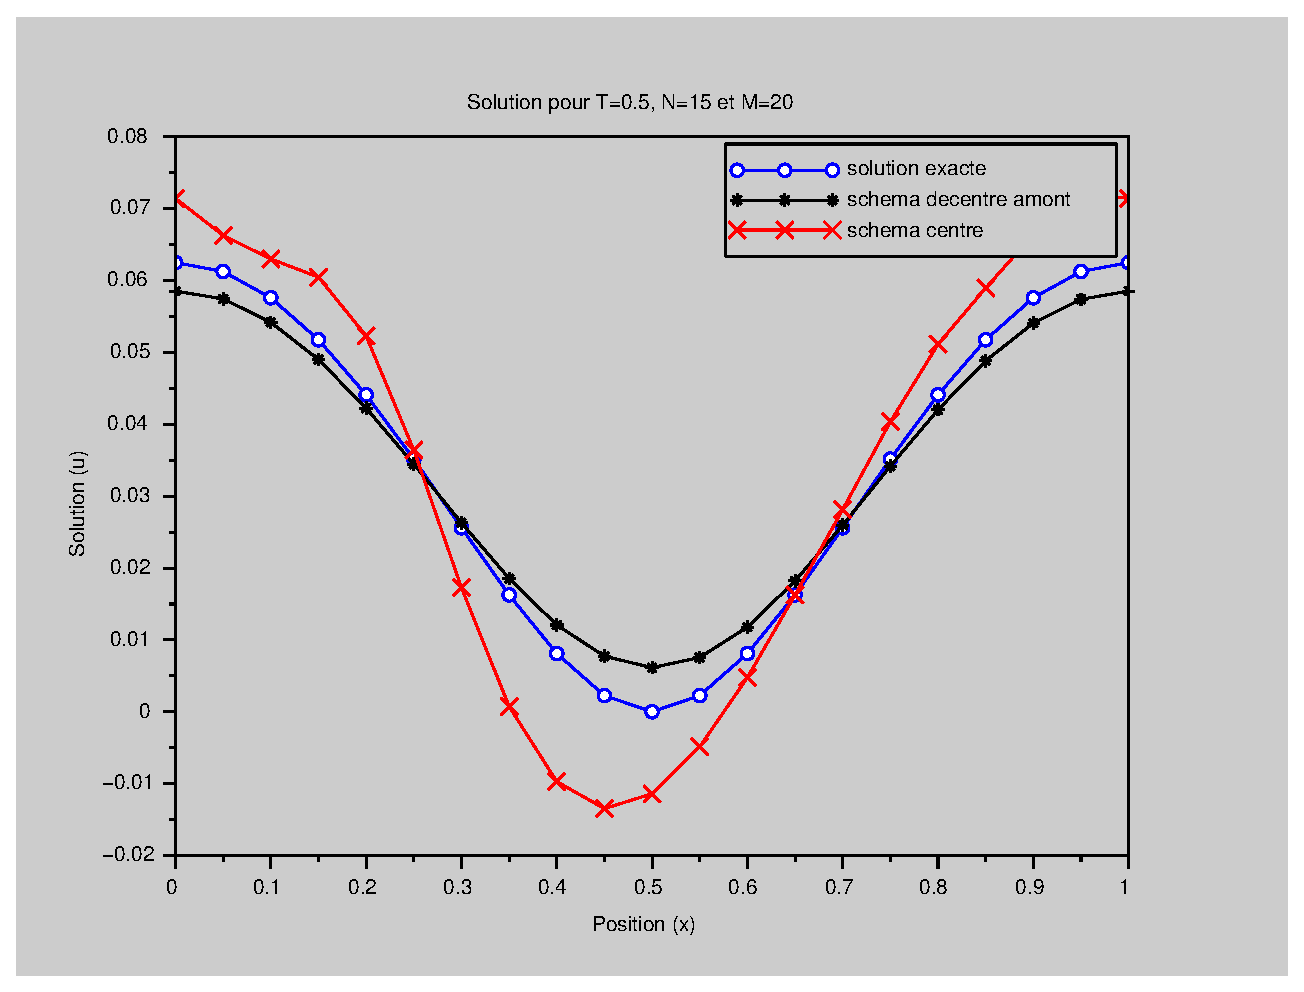
\includegraphics[width = 8cm]{Figures/transport_per_N15.eps}
  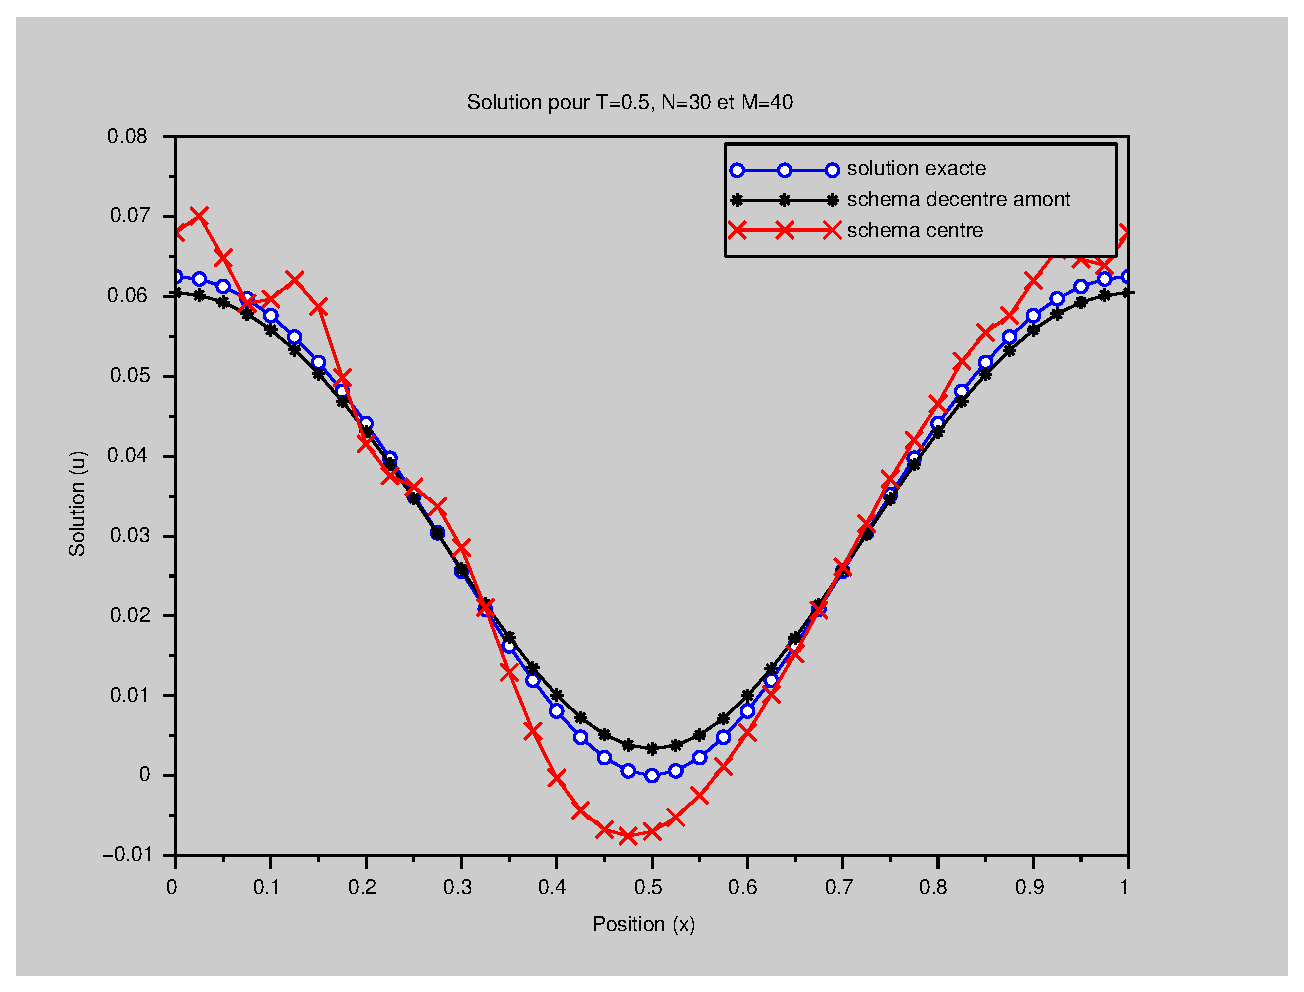
\includegraphics[width = 8cm]{Figures/transport_per_N30.eps}
  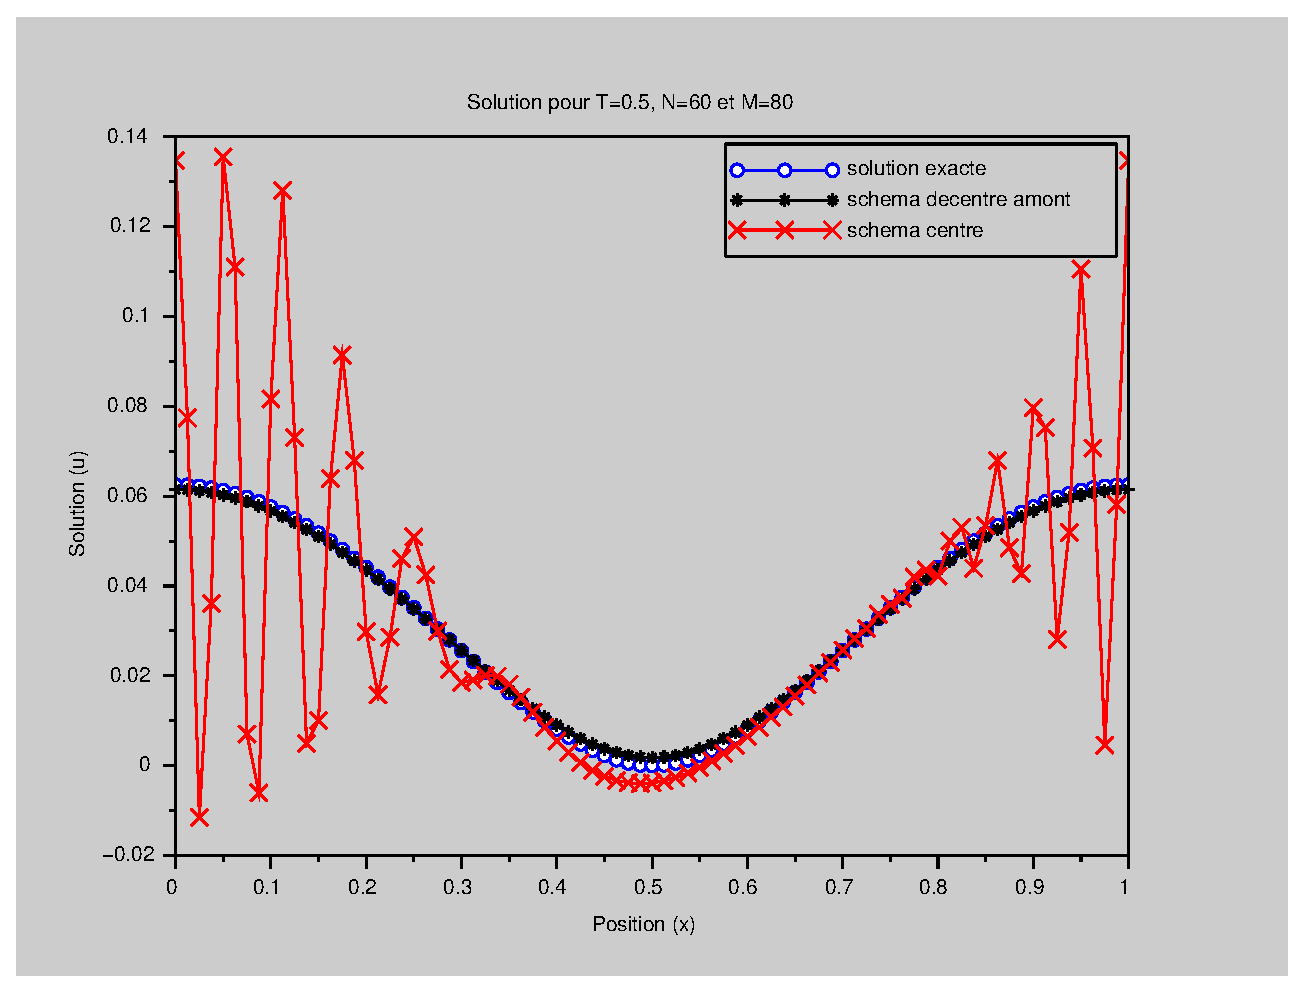
\includegraphics[width = 8cm]{Figures/transport_per_N60.eps}
  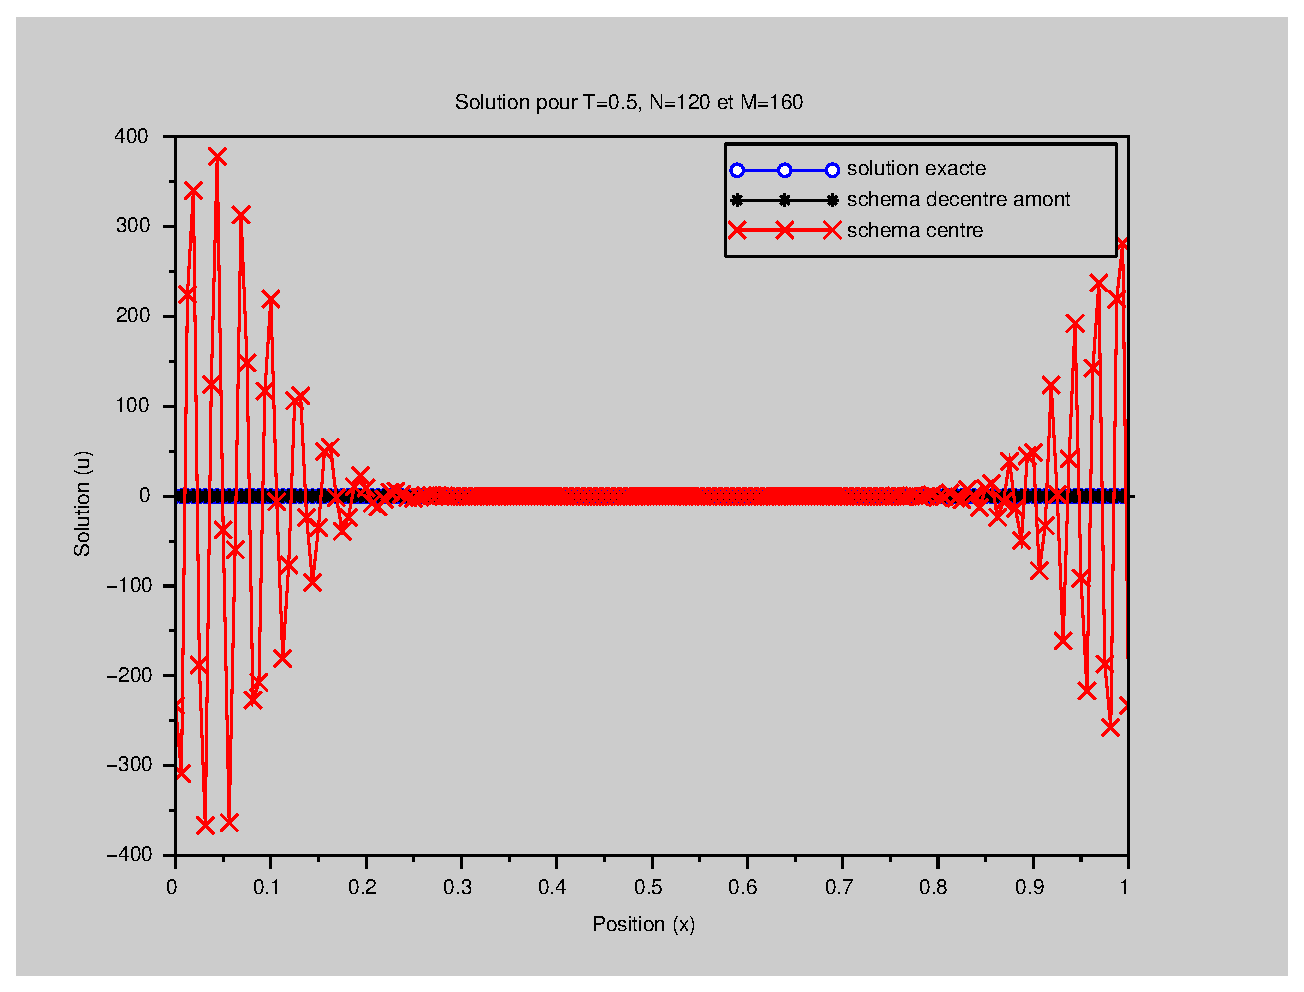
\includegraphics[width = 8cm]{Figures/transport_per_N120.eps}
  \caption{\'Equation de transport avec conditions p\'eriodiques: solution exacte (\`a 
    l'instant final) et
    solutions (\`a l'instant final) 
    obtenues par les sch\'emas d\'ecentr\'e et centr\'e pour $T=0.5$, $a=1$ et
    $(N,M) = (15,20)$, $(30,40)$, $(60,80)$ et $(120,160)$.}
  \label{fig:trans_per}
\end{figure}


Il va de soi que le sch\'ema d\'ecentr\'e a un comportement tout \`a fait acceptable
tandis que le sch\'ema centr\'e est totalement inutilisable.
Il ne suffit donc pas de remplacer les d\'eriv\'ees
partielles de l'EDP par des taux d'accroissement pour obtenir un bon sch\'ema num\'erique.
Pour \^etre s\^ur que le sch\'ema que l'on con\c{c}oit a un bon comportement,
il faut v\'erifier certaines propri\'et\'es que nous allons aborder dans la section suivante.


\begin{exercise}
  La figure \ref{fig:trans_per} a \'et\'e obtenue pour $a=1$, $T=0.5$, $u_0(x) = x^2(1-x^2)$
  et $(N,M) = (15,20)$, $(30,40)$, $(60,80)$ et $(120,160)$.
  Dans ces conditions la solution exacte est $u(t,x) = u_0(f(x-at))$
  (voir exercice \ref{exo:carac_per}).
  Coder les sch\'emas \eqref{eq:transport_DF_centre} et \eqref{eq:transport_DF_decentre_AM}
  et retrouver la figure \ref{fig:trans_per}.
  On pourra aussi explorer d'autres valeurs de $(N,M)$.
\end{exercise}

%%%%%%%%%%%%%%%%%%
\subsubsection{Analyse num\'erique : d\'efinitions et th\'eor\`emes}
\label{subsubsec:analyse_def}

Nous d\'efinissons maintenant des notions que nous
utilisons ensuite pour analyser les deux sch\'emas introduits pr\'ec\'edemment.
Pour cela, repr\'esentons la suite $(u_j^n)_{\substack{0 \leq n \leq N \\ 0 \leq j \leq M}}$
par un vecteur $U^n$
tel que $u_j^n$ soit \'egal \`a la $j$-\`eme coordonn\'ee du vecteur
$U^n$ g\'en\'er\'e par r\'ecurrence comme suit:
\begin{align}
  \label{eq:schema_1pas}
  U^0 = U_0 \qquad \text{et} \qquad \forall n \geq 0, \quad U^{n+1} = A U^n + h_t F^n ,
\end{align}
o\`u $U_0$ est donn\'e par $(U_0)_j = u(0,x_j)$, $A$ est une matrice
et $F^n$ est un vecteur.
Afin de simplifier notre propos, nous consid\'erons que le syst\`eme \`a inverser 
a $M$ inconnues que l'on num\'erotera de $1$ \`a $M$.
Ainsi, pour tout $0 \leq n \leq N$,
$U^n \in \R^M$ avec $\forall 1 \leq j \leq M$, $(U^n)_j = u_j^n$ et de m\^eme
$A \in \R^{M \times M}$ et $F^n \in \R^M$.
La valeur de $u_0^n$ n'est pas consid\'er\'ee comme inconnue du probl\`eme
car elle est donn\'ee par une condition limite (Dirichlet ou p\'eriodique).
Si le syst\`eme dispose d'un nombre diff\'erent d'inconnues, on pourra
ais\'ement adapter notre propos.

\begin{remark}
  Dans le cas pr\'esent, nous consid\'erons une suite dont la formule de r\'ecurrence
  ne n\'ecessite que le pas de temps pr\'ec\'edent (sch\'ema \`a un pas de temps).
  En pratique, certains sch\'emas n\'ecessitent plusieurs pas de temps pr\'ec\'edents.
  Le sch\'ema \eqref{eq:schema_1pas} ainsi que les notions que nous abordons dans cette
  section peuvent \^etre adapt\'es \`a ce cas de figure.
  Nous verrons ceci plus loin dans ce cours.
\end{remark}

D\'efinissons maintenant un certain nombre de notions utiles pour
\'etudier le comportement du sch\'ema \eqref{eq:schema_1pas}.
\begin{definition}[Stabilit\'e]
  \label{def:stabilite}
  Soit $\Stab \subset \R_+^* \times \R_+^*$ tel que $(0,0) \in \overline{\Stab}$.
  On dit que le sch\'ema num\'erique \eqref{eq:schema_1pas} est stable 
  sous la condition $\Stab$ s'il existe $C_1 , C_2 > 0$ qui ne d\'ependent que de $T$
  tels que $\forall (h_x , h_t) \in \Stab$, $\forall U_0 \in \R^{M}$, 
  $\forall (F^n)_{0 \leq n \leq N} \in \R^{(N+1) \times M}$, on a
  \begin{align}
    \max_{\substack{0\leq n \leq N\\ 1 \leq j \leq M}} | u_j^n | 
    \leq C_1 \max_{1 \leq j \leq M} | (U_0)_j | 
    + C_2 \max_{\substack{0\leq n \leq N\\ 1 \leq j \leq M}} | F_j^n | ,
  \end{align}
  o\`u $u_j^n = (U^n)_j$ avec $(U^n)$ l'unique suite v\'erifiant \eqref{eq:schema_1pas}.

  On dit \'egalement que le sch\'ema \eqref{eq:schema_1pas} 
  est inconditionnellement stable
  si la d\'efinition pr\'ec\'edente
  s'applique avec $\Stab = \R_+^* \times \R_+^*$.
\end{definition}

\begin{definition}[Erreur de troncature]
  \label{def:troncature}
  L'erreur de troncature (ou erreur de consistance) du sch\'ema \eqref{eq:schema_1pas}
  au temps $t_n$ est un vecteur $\varepsilon^n \in \R^{M}$
  ($1 \leq n \leq N$)
  d\'efini par
  \begin{align}
    \label{eq:troncature}
    \varepsilon^{n+1} := \tu^{n+1} - A \tu^n - h_t F^n ,
  \end{align}
  o\`u $\tu^n \in \R^{M}$ est d\'efini par
  $(\tu^n)_j = u(t_n,x_j)$ avec $u$ la solution du probl\`eme exact associ\'e \`a
  \eqref{eq:schema_1pas}.
\end{definition}

\begin{definition}[Consistance]
  \label{def:consistance}
  On dit que le sch\'ema num\'erique \eqref{eq:schema_1pas} est consistant si pour toute
  solution r\'eguli\`ere $u$ du probl\`eme exact on a
  \begin{align}
    \lim_{\substack{N \to +\infty\\ M \to +\infty}} \max_{\substack{0\leq n \leq N\\ 1 \leq j \leq M}} 
    \dfrac{| \varepsilon_j^n|}{h_t} = 0 ,
  \end{align}
  o\`u $\varepsilon_j^n = (\varepsilon^n)_j$ est l'erreur de troncature
  (et $h_t = T/N$).

  On dit de plus que le sch\'ema \eqref{eq:schema_1pas} est consistant d'ordre $p \in \N^*$
  en temps et $q \in \N^*$ en espace si pour toute solution r\'eguli\`ere $u$ (du probl\`eme exact)
  il existe une constante $C>0$ ind\'ependante de $h_t$ et $h_x$ telle que
  \begin{align}
    \forall N, M \geq 2 , \quad \max_{\substack{0\leq n \leq N\\ 1 \leq j \leq M}}
    \dfrac{| \varepsilon_j^n|}{h_t} \leq C (h_t^p + h_x^q) .
  \end{align}
\end{definition}

\begin{remark}
  Notons que la constante $C$ dans la d\'efinition \ref{def:consistance}
  peut d\'ependre de la solution $u$ du probl\`eme exact.
\end{remark}

\begin{definition}[Convergence]
  \label{def:convergence}
  On dit que le sch\'ema num\'erique \eqref{eq:schema_1pas} converge (ou est convergent) 
  sous la condition $\Stab \subset \R_+^* \times \R_+^*$
  si 
  \begin{align}
    \lim_{\substack{(h_t,h_x) \in \Stab \\ (h_t,h_x) \to (0,0)}} \max_{\substack{0\leq n \leq N\\ 1 \leq j \leq M}} 
    | u(t_n , x_j) - u_j^n | = 0 ,
  \end{align}
  avec $Nh_t = T$ et $Mh_x = 1$ o\`u $u$ est la solution du probl\`eme exact.
  
  De mani\`ere similaire, on dit que le sch\'ema num\'erique 
  \eqref{eq:schema_1pas} converge (ou est convergent) 
  \`a l'ordre $p\in\N^*$ en temps et $q\in\N^*$ en espace
  sous la condition $\Stab \subset \R_+^* \times \R_+^*$
  s'il existe une constante $C>0$ ind\'ependante de $h_t$ et $h_x$
  telle que
  \begin{align}
    \forall (h_t , h_x) \in \Stab , \quad \max_{\substack{0\leq n \leq N\\ 1 \leq j \leq M}}
    | u(t_n,x_j) - u_j^n | \leq C (h_t^p + h_x^q) .
  \end{align}

  On dit enfin que le sch\'ema est convergent (resp. convergent \`a l'ordre $p$
  en temps et $q$ en espace) si la d\'efinition ci-dessus est v\'erifi\'ee
  avec $\Stab = \R_+^* \times \R_+^*$.
\end{definition}

Ces d\'efinitions sont reli\'ees par le th\'eor\`eme de Lax.
\begin{theorem}[Th\'eor\`eme de Lax]
  \label{thm:convergence}
  Si le sch\'ema \eqref{eq:schema_1pas} est stable sous la condition
  $\Stab \subset \R_+^* \times \R_+^*$ et consistant 
  (respectivement consistant d'ordre $p$ en temps et $q$ en espace),
  alors le sch\'ema \eqref{eq:schema_1pas} est convergent
  (respectivement convergent d'ordre $p$ en temps et $q$ en espace)
  sous la condition $\Stab$.


  De plus, si le probl\`eme exact (le probl\`eme v\'erifi\'e par $u$) 
  est bien pos\'e, alors la consistance et la stabilit\'e du sch\'ema 
  sont n\'ecessaires \`a sa convergence.
\end{theorem}
Le th\'eor\`eme \ref{thm:convergence} s'applique aussi avec $\Stab = \R_+^* \times \R_+^*$.
Avant d'exposer une preuve de ce th\'eor\`eme 
faisons quelques remarques sur les d\'efinitions pr\'ec\'edentes.


Concernant la stabilit\'e (cf d\'efinition \ref{def:stabilite}),
les quantit\'es $\max_{\substack{0\leq n \leq N\\ 1 \leq j \leq M}} | u_j^n |$, 
$\max_{1\leq j \leq M} | (U_0)_j |$ et $\max_{\substack{0\leq n \leq N\\ 1 \leq j \leq M}} | F_j^n |$ 
sont des normes portant sur $(u_j^n)$, $U_0$ et $(F^n)$.
On peut dire que la stabilit\'e du sch\'ema correspond \`a
la continuit\'e de l'application lin\'eaire qui \`a 
$U_0$ et $(F^n)$ associe $(u_j^n)$ 
avec une constante de continuit\'e que ne d\'epend pas
de $h_t$ et $h_x$.
Cette continuit\'e permet d'obtenir le fait qu'une "petite"
modification de la donn\'ee initiale ou des termes $F^n$
ne cr\'ee qu'une "petite" modification
du r\'esultat obtenu et que cette propri\'et\'e se conserve lorsque
$(h_t,h_x) \to (0,0)$.
Remarquons sur la figure \ref{fig:trans_per} que l'erreur commise
par le sch\'ema centr\'e augmente fortement lorsque
$(h_t,h_x) \to (0,0)$, nous verrons plus loin que ce comportement
est d\^u \`a un d\'efaut de stabilit\'e.


La condition $\Stab$ permet de traiter des cas o\`u le sch\'ema
n'est stable que si on restreint les $h_t$ et $h_x$ utilis\'es.
Nous verrons dans la suite de cette section que le sch\'ema 
d\'ecentr\'e amont \eqref{eq:transport_DF_decentre_AM} 
n'est stable que sous une certaine condition
que nous expliciterons.


On pourrait consid\'erer d'autres normes pour exprimer cette stabilit\'e.
Par exemple, on pourrait consid\'erer la norme
$\max_{0\leq n \leq N} \sqrt{h_x} (\sum_{0\leq j \leq M} (u_j^n)^2)^{1/2}$
pour $(u_j^n)$.
La d\'efinition propos\'ee ne serait alors pas n\'ecessairement
\'equivalente \`a celle de la d\'efinition \ref{def:stabilite}.
En effet, si toutes les normes sont \'equivalentes en dimension
finie, rien ne prouve que les constantes de la relation
d'\'equivalence ne d\'ependent pas de $h_t$ et $h_x$.




L'erreur de troncature repr\'esente l'erreur que fait le sch\'ema
au cours d'un pas de temps en partant de la solution exacte.
En effet, on compare (cf d\'efinition \ref{def:troncature})
la solution exacte $\tu^{n+1}$ \`a la solution 
obtenue en faisant un pas de temps du sch\'ema
\`a partir de la solution exacte au pas de temps
pr\'ec\'edent $\tu^{n}$.


La consistance d'un sch\'ema (cf d\'efinition \ref{def:consistance})
signifie que l'erreur de troncature commise par unit\'e de temps
(on divise par $h_t$) tend vers $0$ lorsque $(h_t,h_x) \to (0,0)$.
De plus, on peut quantifier la notion de consistance
gr\^ace \`a l'ordre de consistance 
(plus les ordres de consistance en temps et en espace sont \'elev\'es,
plus l'erreur de troncature d\'ecro\^it vite vers $0$ quand $(h_t,h_x) \to (0,0)$).
En quelque sorte, la consistance signifie que le sch\'ema est
coh\'erent avec le probl\`eme exact 
(les termes pr\'esents dans le sch\'ema num\'erique correspondent
\`a des termes du probl\`eme exact et vice-versa).


La convergence d'un sch\'ema signifie que la solution approch\'ee obtenue
correspond bien \`a une approximation de la solution exacte
au sens o\`u si l'on fait tendre les pas de temps et d'espace vers
$0$, l'erreur commise par le sch\'ema tend aussi vers $0$.
L\`a encore on peut quantifier cette d\'ecroissance de l'erreur commise 
avec la notion d'ordre de convergence.
\'Etant donn\'e que les ordres de consistance et de convergence 
se correspondent (voir th\'eor\`eme \ref{thm:convergence}), 
on parle parfois simplement d'ordre d'un sch\'ema
(sans pr\'eciser 'convergence' ou 'consistance').


En pratique, la convergence est la propri\'et\'e que l'on veut avoir
car elle garantit que le sch\'ema consid\'er\'e fournit une approximation
raisonnable du probl\`eme exact (sous r\'eserve que les pas de temps
et d'espace sont suffisamment petits).
Cependant, cette propri\'et\'e n'est pas ais\'ee \`a d\'emontrer.
C'est pourquoi nous utilisons le th\'eor\`eme \ref{thm:convergence}
qui assure la convergence \`a partir de la stabilit\'e et 
de la consistance.
Notons \'egalement que si le probl\`eme exact est bien pos\'e
alors avoir la convergence est \'equivalent \`a avoir
la stabilit\'e et la consistance.
Ceci signifie qu'en pratique, on ne peut pas esp\'erer avoir un sch\'ema convergent
s'il manque la consistance ou la stabilit\'e.


\begin{remark}
  Les notions de consistance et de convergence sont diff\'erentes.
  Les jurys se plaignent des candidats qui confondent ces deux
  notions.
  Ne fa\^ites pas cette erreur.
\end{remark}

\begin{remark}
  Toutes ces d\'efinitions caract\'erisent le comportement du sch\'ema 
  lorsque $(h_t,h_x) \to (0,0)$.
  En g\'en\'eral, l'analyse num\'erique n'est men\'ee que dans cette limite.
\end{remark}

Nous allons maintenant prouver la premi\`ere partie du th\'eor\`eme \ref{thm:convergence}
qui est celle que l'on utilise en pratique.
\begin{proof}[Preuve partielle du th\'eor\`eme \ref{thm:convergence}]
  Dans cette preuve, nous utilisons toutes les d\'efinitions pr\'ec\'edentes.
  Tout d'abord, par d\'efinition de l'erreur de troncature,
  $\tu^{n+1} = A \tu^n + h_t F^n + \varepsilon^{n+1}$.
  On montre ainsi que
  $w^n = \tu^{n} - U^{n}$ v\'erifie $w^0 = 0$ 
  (puisque $(U^0)_j = u(t_0,x_j)$) et
  $w^{n+1} = A w^n + \varepsilon^{n+1}$.

  Par stabilit\'e du sch\'ema, on obtient
  $\max_{\substack{0\leq n \leq N\\ 1 \leq j \leq M}} | w_j^n |
  \leq C_2 \max_{\substack{0\leq n \leq N\\ 1 \leq j \leq M}} \dfrac{| \varepsilon_j^n |}{h_t}$.
  On conclut en utilisant la d\'efinition de la consistance.
\end{proof}



Comme nous l'avons dit, en pratique, pour prouver la convergence du sch\'ema
on prouve sa consistance et sa stabilit\'e.
Il se trouve que les preuves de consistances sont g\'en\'eralement plut\^ot
ais\'ees, la difficult\'e se trouve donc plut\^ot dans la preuve de la stabilit\'e.
Afin de faciliter ces preuves,
nous en donnons maintenant des conditions n\'ecessaires et des conditions
suffisantes.
Pour $A \in \R^{M \times M}$, on note 
$\tn A \tn = \sup_{V \in \R^{M} \backslash\{0\}} \dfrac{\| A V \|}{\| V \|}$,
o\`u $\| V \| = \max\limits_{1 \leq j \leq M} | V_j |$.
Rappelons que $\tn \cdot \tn$ est une norme sur $\R^{M \times M}$.
Commen\c{c}ons d'abord par le r\'esultat suivant.
\begin{proposition}
  \label{prop:carac_stab}
  Le sch\'ema \eqref{eq:schema_1pas} est stable si et seulement si
  il existe $C>0$ d\'ependant uniquement de $T$ tel que
  \begin{align}
    \label{eq:carac_stab}
    \forall n \in \N , \quad \tn A^n \tn \leq C .
  \end{align}
\end{proposition}

\begin{corrolary}
  \label{corro:stability}
  Si $\tn A \tn \leq 1$, alors le sch\'ema est stable.
\end{corrolary}

\begin{proof}[Preuve de la proposition \ref{prop:carac_stab}]
  Supposons tout d'abord que le sch\'ema est stable.
  Dans ce cas, appliquons le sch\'ema \`a $U_0 = V \in \R^{M}$
  quelconque et $F^n = 0$. 
  La solution obtenue est $U^n = A^n V$.
  On a donc prouv\'e qu'il existe $C>0$ d\'ependant uniquement
  de $T$ tel que
  $\forall V \in \R^{M} , \quad \| A^n V \| \leq C \| V \|$
  et donc \eqref{eq:carac_stab}.

  Maintenant supposons que \eqref{eq:carac_stab} est \'etablie.
  Appliquons le sch\'ema \`a $U_0 \in \R^{M}$
  et $(F^n) \in \R^{(N+1) \times M}$.
  Nous pouvons prouver (voir exercice \ref{exo:sol_schema_1pas}) 
  que la solution obtenue est donn\'ee par
  \begin{align*}
    \forall 0 \leq n \leq N , \quad U^n = A^n U_0 + h_t \sum_{\ell = 0}^{n-1} A^{n-\ell-1} F^{\ell} .
  \end{align*}
  Ainsi, $\| U^n \| \leq \tn A^n \tn \| U_0 \| 
  + h_t \sum_{\ell = 0}^{n-1} \tn A^{n-\ell-1} \tn \| F^n \|$.
  En utilisant \eqref{eq:carac_stab}, on obtient
  $\| U^n \| \leq C \| U_0 \| + C h_t n \max_{0\leq \ell \leq N} \| F^{\ell} \|$,
  avec $C$ la constante de \eqref{eq:carac_stab} qui d\'epend
  uniquement de $T$.
  De plus, $n h_t = t_n \leq T$.
  On a donc \'etabli la stabilit\'e du sch\'ema.
\end{proof}


\begin{exercise}
  \label{exo:sol_schema_1pas}
  Soient $U_0 \in \R^{M}$ et $(F^n) \in \R^{(N+1) \times M}$.
  Montrer que l'unique solution de \eqref{eq:schema_1pas}
  est donn\'ee par
  \begin{align}
    \label{eq:sol_Un}
    \forall 0 \leq n \leq N , \quad  U^n = A^n U_0 + h_t \sum_{\ell = 0}^{n-1} A^{n-\ell-1} F^{\ell} .
  \end{align}
\end{exercise}


Nous introduisons une derni\`ere d\'efinition: la stabilit\'e
au sens de Von Neumann.
Lorsque l'on veut prouver qu'un sch\'ema de la forme \eqref{eq:schema_1pas}
est instable, la fa\c{c}on standard
de proc\'eder est de montrer qu'il n'est pas stable au sens de Von Neumann.
On consid\`ere alors $F^n = 0$ et une condition initiale sous la forme
d'une onde spatiale: $u_j^0 = e^{2 i \pi k x_j}$ avec $i$ la racine carr\'e de l'unit\'e
et $k \in \Z$.
On \'etudie ensuite l'effet qu'a l'application du sch\'ema sur cette condition initiale complexe.

L'int\'er\^et de choisir un vecteur de la forme $u_j^0 = e^{2 i \pi k x_j}$
est que l'on a $u_j^1 = \sum_{\ell=1}^{M} a_{j \ell} u_{\ell}^{0}$.
En prenant $\calA_j(k) = \sum_{\ell=1}^{M} a_{j\ell} e^{2i\pi k (x_{\ell} - x_j)}$, on montre
que $\forall 1\leq j \leq M, \;  u_j^{1} = \calA_j(k) u_j^0$ avec $\calA_j(k) \in \C$.
\begin{definition}[Stabilit\'e au sens de Von Neumann]
  On dit qu'un sch\'ema \eqref{eq:schema_1pas} est stable au
  sens de Von Neumann si pour tout $1 \leq j \leq M$ 
  et pour tout $k \in \Z$, $| \calA_j(k) | \leq 1$.
\end{definition}
\begin{proposition}
  \label{prop:Von_Neumann_nec}
  La stabilit\'e au sens de Von Neumann est n\'ecessaire \`a la stabilit\'e du sch\'ema.
  Dit autrement, la stabilit\'e du sch\'ema implique la stabilit\'e au sens de 
  Von Neumann.
\end{proposition}
\begin{proof}
  On peut montrer que si on consid\`ere $u_j^0 = \Re (e^{2 i \pi k x_j})$
  et $F^n = 0$
  alors $\forall 0 \leq n \leq N, u_j^n = \Re ((\calA_j(k))^n e^{2 i \pi k x_j})$.
  Idem, si $u_j^0 = \Im (e^{2 i \pi k x_j})$, 
  alors $\forall 0 \leq n \leq N, u_j^n = \Im ((\calA_j(k))^n e^{2 i \pi k x_j})$.
  
  Ainsi, si le sch\'ema \eqref{eq:schema_1pas} est stable alors
  $\max_{\substack{0 \leq n \leq N \\ 1 \leq j \leq M}} 
  | \Re ((\calA_j(k))^n e^{2 i \pi k x_j})| \leq C$ o\`u $C>0$ ne d\'epend que de $T$.
  En faisant le m\^eme raisonnement sur la partie imaginaire,
  on obtient
  $\max_{\substack{0 \leq n \leq N \\ 1 \leq j \leq M}} 
  | (\calA_j(k))^n e^{2 i \pi k x_j}| \leq \sqrt{2}C$.
  
  Or ceci n'est possible que si $| \calA_j(k) | \leq 1$ sinon on d\'epasse
  la constante $\sqrt{2}C$ en faisant tendre $N$ vers $+\infty$.
  Ceci prouve le r\'esultat.
\end{proof}


Par la suite nous utilisons la stabilit\'e de Von Neumann lorsque nous voulons 
prouver qu'un sch\'ema n'est pas stable.

\begin{remark}
  On peut prouver que la
  stabilit\'e de Von Neumann correspond \`a la stabilit\'e du sch\'ema 
  dans le sens $\| (u_j^n) \|_{*} \leq C_1 \| U_0 \|_{\#} + C_2 \| (F^n) \|_{*}$,
  avec $C_1$ et $C_2$ ne d\'ependant que de $T$
  et des normes $\| \cdot \|_{*}$ et $\| \cdot \|_{\#}$ diff\'erentes de celles
  de la d\'efinition \ref{def:stabilite}.
\end{remark}

%%%%%%%%%%%%%%%%%%
\subsubsection{Analyse des deux sch\'emas donn\'es en introduction}


Nous allons montrer dans cette section que le sch\'ema num\'erique 
propos\'e en \eqref{eq:transport_DF_centre} n'est pas stable
contrairement au sch\'ema \eqref{eq:transport_DF_decentre_AM}.
C'est ce d\'efaut de stabilit\'e qui explique son mauvais comportement.

On consid\`ere comme degr\'es de libert\'e
$U^n = 
\begin{pmatrix}
  u_1^n \\ \vdots \\ u_{M}^n
\end{pmatrix}
\in \R^M
$.
Les deux sch\'emas pr\'ec\'edents peuvent \^etre \'ecrits sous la forme matricielle 
\eqref{eq:schema_1pas} avec $F^n = 0$ et
\begin{align}
  A_{C} = \dfrac{1}{2}
  \begin{pmatrix}
    2 & -\co & 0 & \dots & 0 & \co
    \\
    \co & 2 & -\co & & & 0
    \\
    0 & \ddots & \ddots & \ddots & &
    \\
    \vdots & & \ddots & \ddots & \ddots
    \\
    0 & & & \ddots & \ddots & -\co
    \\
    -\co & 0 & & & \co & 2
  \end{pmatrix},
\end{align}
pour le sch\'ema centr\'e \eqref{eq:transport_DF_centre}
et
\begin{align}
  A_{AM} = 
  \begin{pmatrix}
    1-\co & 0 & \dots & 0 & \co
    \\
    \co & \ddots & & & 0
    \\
    & \ddots & \ddots &   &
    \\
    & & \ddots & \ddots &
    \\
    &&   &  \co & 1-\co
  \end{pmatrix},
\end{align}
pour le sch\'ema d\'ecentr\'e amont \eqref{eq:transport_DF_decentre_AM}.
Les deux matrices pr\'ec\'edentes sont dans
$\R^{M \times M}$ et ont \'et\'e \'ecrites avec 
$\co = \frac{a h_t}{h_x}$.

\begin{proposition}
  \label{prop:consistance_2_schemas}
  Les sch\'emas \eqref{eq:transport_DF_centre} et \eqref{eq:transport_DF_decentre_AM}
  sont tous les deux consistants.
  De plus, le sch\'ema \eqref{eq:transport_DF_centre} est consistant d'ordre 1
  en temps et 2 en espace;
  le sch\'ema \eqref{eq:transport_DF_decentre_AM} est consistant d'ordre 1
  en temps et 1 en espace.
\end{proposition}


\begin{proof}
  Prouvons que le sch\'ema \eqref{eq:transport_DF_centre} est consistant
  d'ordre 1 en temps et 2 en espace.
  La preuve pour le sch\'ema d\'ecentr\'e amont est laiss\'ee en exercice
  (cf exercice \ref{exo:consistance_trans_AM}).

  On calcule l'erreur de troncature. Ceci revient \`a 
  calculer une solution approch\'ee au temps $t_{n+1}$ par le sch\'ema \`a partir
  de la solution exacte au temps $t_n$ et de comparer le r\'esultat
  obtenu \`a la solution exacte au temps $t_{n+1}$.
  On a ainsi
  \[
    \varepsilon_j^{n+1} = u(t_{n+1},x_j) - u(t_n,x_j)
    + \dfrac{a h_t}{2 h_x} (u(t_n, x_{j+1}) - u(t_n, x_{j-1})) ,
  \]
  o\`u $u$ est la solution de \eqref{eq:transport_per}.

  On consid\`ere ensuite les d\'eveloppements de Taylor suivants:
  \begin{align*}
    u(t_{n+1} , x_j) = u(t_n , x_j) + h_t \dfrac{\partial u}{\partial t} (t_n , x_j)
    + O(h_t^2) ,
    \\
    u(t_n , x_{j+1} ) = u(t_n , x_{j} ) + h_x \dfrac{\partial u}{\partial x}(t_n, x_j)
    + \dfrac{h_x^2}{2} \dfrac{\partial^2 u}{\partial x^2}(t_n, x_j)
    + O(h_x^3) ,
    \\
    u(t_{n} , x_{j-1} ) = u(t_n , x_{j} ) - h_x \dfrac{\partial u}{\partial x}(t_n, x_j)
    + \dfrac{h_x^2}{2} \dfrac{\partial^2 u}{\partial x^2}(t_n, x_j)
    + O(h_x^3) .
  \end{align*}
  Nous obtenons donc
  \begin{align*}
    \dfrac{\varepsilon_j^{n+1}}{h_t} = \dfrac{\partial u}{\partial t}(t_n, x_j)
    + O (h_t) + a \dfrac{\partial u}{\partial x}(t_n, x_j) + O (h_x^2) .
  \end{align*}
  En utilisant le fait que $u$ est solution de \eqref{eq:transport_per},
  on a 
  $\dfrac{\partial u}{\partial t}(t_n, x_j) + a \dfrac{\partial u}{\partial x}(t_n, x_j) = 0$.
  Nous avons prouv\'e le fait que le sch\'ema \eqref{eq:transport_DF_centre}
  est consistant d'ordre 2 en espace et d'ordre 1 en temps.
\end{proof}

\begin{exercise}
  \label{exo:consistance_trans_AM}
  Terminer la preuve de la proposition \ref{prop:consistance_2_schemas}:
  prouver que le sch\'ema \eqref{eq:transport_DF_decentre_AM} est consistant
  d'ordre 1 en temps et en espace. 
\end{exercise}


\begin{proposition}
  \label{prop:stabilite_transport_AM}
  Le sch\'ema \eqref{eq:transport_DF_decentre_AM} est stable
  sous la condition $c = \dfrac{a h_t}{h_x} \leq 1$.
  De plus, ce sch\'ema est instable si $c > 1$.
\end{proposition}
\begin{proof}
  Supposons $c \leq 1$ et montrons que le sch\'ema est stable.
  Soit $U_0 \in \R^M$, on calcule $U^1 = A U_0$.
  Pour $1 \leq j \leq M$, 
  $u_j^1 = (1-c) u_j^0 + c u_{j-1}^0$.
  Ainsi, $|u_j^1| \leq |1-c| | u_j^0 | + | c | | u_{j-1}^0 |$.
  On obtient $\| U^1 \| \leq (|1-c| + |c|) \| U_0 \|$.
  Ceci \'etant valide pour tout $U_0 \in \R^M$, on a $\tn A \tn \leq |1-c| + |c|$.
  La condition $0 \leq c \leq 1$ donne $\tn A \tn \leq 1$ et le sch\'ema est stable 
  d'apr\`es le corrolaire \ref{corro:stability}.

  Supposons maintenant que $c > 1$ et montrons que le sch\'ema est instable.
  Pour cela, nous allons montrer qu'il est instable au sens de Von Neumann.
  Si $u_j^0 = e^{2i\pi k x_j}$, alors
  \[
    u_j^{1} = (1-c) u_j^0 + c u_{j-1}^0 = (1 - c + c e^{-2i\pi k h_x}) u_j^0 
    = \calA(k) u_j^0.
  \]
  Ici, nous avons $\calA(k) = 1 - c + c e^{-2i\pi k h_x}$.
  Pour $c > 1$ et $k=1$, on a pour $h_x<1$,
  $| \calA | > 1$ (on montre que $\cos(2\pi k h_x) < 1$). 
  Le sch\'ema n'est pas stable au sens 
  de Von Neumann donc, d'apr\`es la proposition \ref{prop:Von_Neumann_nec},
  il n'est pas stable au sens de la d\'efinition \ref{def:stabilite}.
\end{proof}

La mauvais comportement du sch\'ema centr\'e provient d'un d\'efaut
de stabilit\'e. La preuve de ce r\'esultat est laiss\'ee en exercice.
\begin{exercise}[Instabilit\'e du sch\'ema explicite centr\'e]
  Montrer que le sch\'ema \eqref{eq:transport_DF_centre} est instable
  (c'est-\`a-dire n'est stable sous aucune condition $\Stab$).
\end{exercise}


!! FIN DE L'ENVOI !!



Nous pouvons tirer plusieurs conclusions de l'\'etude de ces deux sch\'emas.
Tout d'abord, le fait de d\'ecentrer la d\'eriv\'ee partielle en espace
a permis de rendre le sch\'ema stable.
Notons que le sens dans le lequel on d\'ecentre cette d\'eriv\'ee est essentiel,
on peut montrer que le sch\'ema d\'ecentr\'e aval est instable pour 
$a>0$ et qu'il faut changer le sens du d\'ecentrage si $a<0$.
En fait, il faut d\'ecentrer en utilisant les donn\'ees qui correspondent
\`a de l'information qui arrive et non de l'information qui part.


De plus, nous avons vu dans la proposition \ref{prop:stabilite_transport_AM} que
le sch\'ema \eqref{prop:stabilite_transport_AM} est stable
uniquement sous la condition $a h_t \leq h_x$
qui lie les pas de temps et d'espace.
On appelle une telle condition "condition de CFL" pour 
Courant--Friedrichs--Lewy.
De la m\^eme fa\c{c}on on appelle $c = \frac{a h_t}{h_x}$
le nombre de CFL.
De telles conditions doivent \^etre associ\'ees aux sch\'emas
explicites pour esp\'erer les rendre stables.
Seuls les sch\'emas implicites peuvent se passer de ce
type de condition (voir exercice \ref{exo:transport_implicite}).


!! \'etude de l'influence du nombre de cfl (nouvelle section ??) !!
-- DONNER DES FIGURES + EXO : RETROUVER LES FIGURES !!


%%%%%%%%%%%%%%%%%%
\subsubsection{D\'etermination pratique des ordres de convergence}


!! expliquer comment ca marche + figures + exo : retrouver les figures !!

!! Le plus simple est peut-\^etre d'enlever cette section ou au moins la
reporter plus loin dans le poly !!

%%%%%%%%%%%%%%%%%%
\subsubsection{Conditions de Dirichlet}

!! on s'int\'eresse au pb (...) !!

En appliquant \eqref{eq:der_decentre_AM}, 
on obtient le sch\'ema num\'erique
\begin{align}
  \label{eq:transport_DF_decentre_AM_dir}
  \left\{
  \begin{array}{l}
    \forall 0 \leq j \leq M , 
    u_j^0 = u_0(x_j) ,
    \\
    \forall 1 \leq n \leq N, u_0^n = \alpha(t_n) ,
    \\
    \forall 1 \leq n \leq N, \forall 1 \leq j \leq M,
    u_j^n = u_j^{n-1} - \dfrac{a h_t}{h_x} (u_{j}^{n-1} - u_{j-1}^{n-1}) .
  \end{array}
  \right.
\end{align}

On a donc 
\begin{align}
  A =
  \begin{pmatrix}
    1 - \co & 0 & & &
    \\
    \co & 1 - \co & \ddots & &
    \\
    0 & \ddots & \ddots & \ddots &
    \\
    \vdots & & \ddots & \ddots & 0
    \\
    0 & & & \co & 1-\co
  \end{pmatrix}
  \qquad \text{et} \qquad
  \forall n \geq 0,
  \quad h_t F^n = \co
  \begin{pmatrix}
    \alpha(t_n)
    \\
    0
    \\
    \vdots
    \\
    0
  \end{pmatrix}
  ,
\end{align}
avec $\co = \frac{a h_t}{h_x}$.
Remarquons que la condition de Dirichlet a \'et\'e prise en compte
dans le terme "second membre" $F^n$.


!! comparer avec matrice des conditions p\'eriodiques !!


On obtient les r\'esultats (...)

!! est-ce qu'on ne ferait pas mieux de faire l'analyse de stabilit\'e
avec des conditions p\'eriodiques ??
-- Ca simplierait les choses en particulier pour les sch\'emas instables !!


!! remplacer les d\'eriv\'ees continues par des taux d'accroissement
assure la consistance mais pas forc\'ement la stabilit\'e !!
-- C'est tres interessant de faire ca sur l'\'equation de transport par ce que 
l'information ne se d\'eplace que dans une direction !!

!! faire des sous-sections dans cette section !!

!! prouver que le sch\'ema en intro n'est pas stable !!

!! donner un sch\'ema stable sous CFL et faire les preuves + simus num !!

!! introduire nombre de CFL + sens physique + simus avec diff\'erentes CFL !!

!! donner un sch\'ema inconditionnellement stable !!

!! comparer les r\'esultats avec ceux de l'intro !!

!! diffusion num\'erique : comparer avec l'\'equation de la chaleur !!

!! discr\'etisation implicite en exercice !!

!! dessin repr\'esentant l'endroit o\`u on va chercher l'information :
sch\'ema centr\'e / d\'ecentr\'e + effet de la cfl !!

!! faut-il parler des propri\'et\'es de positivit\'e ??
-- OUI ET LE RELIER AVEC LA NOTION DE STABILITE !!

!! exercice sur les ordre de convergence : figure avec echelle logarithmique !!

\begin{exercise}[Sch\'ema implicite]
  \label{exo:transport_implicite}
  Dans cet exercice, on s'int\'eresse \`a une discr\'etisation implicite du probl\`eme
  \eqref{eq:transport}.
  On approche les d\'eriv\'ees partielles en temps et espace
  par des approximations d\'ecentr\'ees amont:
  \begin{align}
    \label{eq:der_decentre_AM2}
    \dfrac{\partial u}{\partial t}(t_n,x_j) \simeq \dfrac{u(t_{n},x_j) - u(t_{n-1},x_j)}{h_t} ,
    \qquad \qquad 
    \dfrac{\partial u}{\partial x}(t_n,x_j) \simeq \dfrac{u(t_n,x_{j}) - u(t_n,x_{j-1})}{h_x} .
  \end{align}
  
  \begin{enumerate}
  \item En consid\'erant la condition de Dirichlet $u(t_n,0) = \alpha(t_n)$, 
    \'ecrire le sch\'ema num\'erique issu de \eqref{eq:der_decentre_AM2}.
    Montrer qu'il peut se mettre sous la forme $\widetilde{A} U^{n} = U^{n-1} + h_t \widetilde{F}^n$.
    Donner $\widetilde{A}$ et $\widetilde{F}^n$.
  \item Montrer que $\widetilde{A}$ est inversible. En d\'eduire que ce sch\'ema v\'erifie
    \eqref{eq:schema_1pas} en donnant $A$ et $F^n$.
    On pourra donc utiliser les d\'efinitions de la section \ref{subsubsec:analyse_def}.
  \item Soit $V \in \R^M$, on note $U = A V$. 
    Calculer les coordonn\'ees de $U$ en fonction de $V$.
    En d\'eduire que $\tn A \tn \leq 1$ et que
    ce sch\'ema est inconditionnellement stable.
    
  \item Montrer que ce sch\'ema est consistant d'ordre 1 en temps et en espace.
    Que peut-on dire de la convergence de ce sch\'ema?

  \item Coder le sch\'ema propos\'e. On peut soit inverser la matrice \`a l'ext\'erieur
    de la boucle en temps, soit r\'esoudre un syst\`eme lin\'eaire \`a chaque pas de temps.
    Comparer les deux m\'ethodes, laquelle est la plus efficace ?
    
    !! Coder ca !!

    NB : commandes scilab


  \item On consid\`ere $a=1$, $u_0 = 0$ et $\alpha(t) = t^2$.
    Quelle est la solution exacte du probl\`eme?
    approcher la solution gr\^ace au sch\'ema implicite.
    Pour $(N,M) = (...)$, que remarquez-vous en $(t,x)=(0.1,0.5)$?
    Si vous l'avez cod\'e, comparez avec le sch\'ema explicite.
    Comment expliquez-vous ceci ?
    
  \item D\'eterminer num\'eriquement le taux de convergence de ce sch\'ema.
    On prendra par exemple la solution du cas test pr\'ec\'edent \`a $T=1$ pour
    estimer la convergence du sch\'ema. Calculer l'erreur et la tracer sur une figure
    \`a l'\'echelle logarithmique comme sur la figure (...).
    Quels ordres de convergence trouvez-vous num\'eriquement ?
  \end{enumerate}
  
  NB : si vous avez des difficult\'es pour l'une de ces questions, vous pouvez \'eventuellement
  lire la section \ref{subsubsec:chaleur_DF_implicite}.

  !! Ajouter une question sur la stabilit\'e de Von Neumann : comparer les preuves des deux stabilit\'es + remarque : Von Neumann plus simple, sera \'etudi\'e dans le chapire suivant (...)
\end{exercise}


%%%%%%%%%%%%%%%%%%%%%%%%%%%%%%%%%%%%%%%%%%%%%%%%%%%%%%%%%%%%%%%%%%%%%%%%%%%%%%%%%%%%
\section{\'Equation de la chaleur}

!! definition des espaces de fonctions utiles : nombre de d\'eriv\'ees en x et en t
peut \^etre diff\'erent !!

\begin{equation}
  \label{eq:chaleur_Dir}
  \text{Trouver $u \in C^2(\Omega)$(...) telle que  }
  \left\{
    \begin{array}{l l}
      \dfrac{\partial u}{\partial t} - \dfrac{\partial^2 u}{\partial x^2} = f 
      &\dans (0,T) \times (0,1) ,
      \\
      u(0,.) = u_0 
      & \dans (0,1) ,
      \\
      u(t,0) = 0 , \quad u(t,1) = 0 & \forall t \in (0,T) ,
    \end{array}
  \right.
\end{equation}
avec (...)


%%%%%%%%%%%%%%%%%%%%%%%%%%%%%%%%%%%%%%%
\subsection{Propri\'et\'es g\'en\'erales}



\begin{theorem}[Existence et unicit\'e de la solution]
  \label{thm:chaleur_existence}
  Supposons que (...).
  Le probl\`eme \eqref{eq:chaleur_Dir} est bien pos\'e:
  il admet une unique solution $u \in $(...)
  et $\| u \| \leq (...)$.

  De plus, cette solution appartient \`a l'espace (...)
\end{theorem}

\begin{remark}[Effet r\'egularisant de l'\'equation de la chaleur]
  Commenter la r\'egularit\'e du th\'eor\`eme. (...)
\end{remark}

\begin{proposition}[Non r\'eversibilit\'e de l'\'equation]
  Le probl\`eme \eqref{eq:chaleur_Dir} n'est pas r\'eversible:
  (...)
\end{proposition}


\begin{proposition}
  \label{prop:chaleur_continuite_donnees}
  Soit $u$ une solution de \eqref{eq:chaleur_Dir},
  alors on a pour tout $t \in [0,T]$,
  \begin{align*}
    \| u(t,.) \|_{(...)} \leq e^{-t} \| u_0 \|_{(...)} + \| f \|_{L^2(]0,t[ \times ]0,1[)} .
  \end{align*}
\end{proposition}

\begin{proof}
  !! TODO !!
\end{proof}


\begin{remark}
  !! \'Energie du syst\`eme (utilis\'e aussi dans le livre de Brigitte Lucquin) !!
  -- Ne correspond pas \`a l'\'energie physique !!
\end{remark}

\begin{remark}
  La continuit\'e par rapport aux donn\'ees traduit une forme de stabilit\'e
  (...)
\end{remark}

\begin{remark}[Conditions de Dirichlet non homog\`enes]
  On peut utiliser un rel\`evement comme dans (...)
\end{remark}

\begin{remark}[Condition de Neumann]
  Conservation de la valeur moyenne ??
  (...)
\end{remark}


\begin{exercise}
  Montrer que la solution du pb de Neumann sans terme source
  tend exponentiellement vers la valeur moyenne de la donn\'ee initiale.
\end{exercise}

%%%%%%%%%%%%%%%%%%%%%%%%%%%%%%%%%%%%%%%
\subsection{Analyse de Fourier}

!! chapeau !!

%%%%%%%%%%%%%%%%
\subsubsection{Recherche d'une solution sous la forme de s\'eries de Fourier}

On cherche une solution r\'eguli\`ere par la m\'ethode de s\'eparation des variables.
On cherche donc une solution de la forme
$u(t,x) = \Phi(t) \Psi(x)$.
Si $f$ est nul, alors on a $\Phi'(t) \Psi(x) = \Phi(t) \Psi''(x)$.
Tant que ces fonctions sont non nulles, on peut \'ecrire
$\frac{\Phi'(t)}{\Phi(t)} = \frac{\Psi''(x)}{\Psi(x)}$.
\'Etant donn\'e que le premier terme d\'epend uniquement de $t$
et le second uniquement de $x$, on peut dire que ces deux termes sont constants.
On suppose que cette constante est non nulle (sinon on a une solution
identiquement nulle).


On a donc les \'equations
$\Phi'(t) = K \Phi(t)$ et $\Psi''(x) = K \Psi(x)$.
Si $K>0$, alors $\Psi(x) = a e^{\sqrt{K} x} + b e^{- \sqrt{K} x}$.
Les conditions aux limites donnent
$a+b=0$ et $a(e^{\sqrt{K}} - e^{-\sqrt{K}}) = 0$.
La seule solution est donc la solution nulle.


On suppose maintenant $K < 0$.
Dans ce cas, $\Psi(x) = a e^{i\sqrt{|K|} x} + b e^{- i\sqrt{|K|} x}$.
Les conditions aux limites donnent alors $a + b = 0$
et $a \sin(\sqrt{|K|}) = 0$.
La seule fa\c{c}on d'avoir une solution non identiquement nulle
est de prendre $K = - \pi^2 k^2$ avec $k \in \Z^*$.


On remarque r\'eciproquement
que les fonctions de la forme $\sin(k \pi x) e^{-k^2 \pi^2 t}$
v\'erifient l'\'equation de la chaleur (avec $f = 0$).
L'approche que nous allons pr\'esenter consiste donc \`a 
chercher une solution au probl\`eme \eqref{eq:chaleur_Dir} sous la forme
d'une s\'erie de ces termes.

On se place ici dans le cas de conditions de Dirichlet homog\`enes
$\alpha = \beta = 0$ et sans terme source $f=0$.
On suppose que la donn\'ee initiale $u_0$ est $C^2([0,1])$ avec $u_0(0) = u_0(1) = 0$.
On note $U_0$ la fonction d\'efinie sur $[-1,1]$ par
\begin{align*}
  U_0(x) =
  \begin{cases}
    u_0(x) \qquad \text{si } x \in [0,1] ,
    \\
    -u_0(-x) \qquad \text{sinon} .
  \end{cases}
\end{align*}
On prolonge \'egalement $U_0$ sur $\R$ par $2$-p\'eriodicit\'e.
La fonction obtenue est $C^1(\R)$.
D'apr\`es le th\'eor\`eme de Dirichlet, cette fonction est donc \'egale \`a 
sa s\'erie de Fourier (qui converge).
De plus, comme $U_0$ est impaire, cette s\'erie de Fourier ne comprends que 
des sinus.

Donc, en particulier, sur $[0,1]$ on a 
\begin{align*}
  u_0(x) = \sum_{k \in \N^*} b_k \sin(k \pi x) ,
\end{align*}
avec
\begin{align*}
  b_k = \dfrac{2}{k \pi} \int_{0}^1 u_0'(x) \cos(k \pi x) \deriv x .
\end{align*}
Comme, pour $t \geq 0$, on a $e^{-k^2 \pi^2 t} \leq 1$, la s\'erie 
$u(t,x) = \sum_{k\in\N^*} b_k \sin(k \pi x) e^{- k^2 \pi^2 t}$ est normalement
convergente sur tout intervalle de la forme
$[a,T] \times [0,1]$ pour tout $a > 0$.
La fonction $u$ est donc d\'erivable par rapport \`a la variable $t$
et sa d\'eriv\'ee est donn\'ee par
\begin{align*}
  \dfrac{\partial u}{\partial t} (t,x) 
  = - \sum_{k \in \N^*} k^2 \pi^2 b_k \sin(k \pi x) e^{-k^2 \pi^2 t} .
\end{align*}
On peut \'egalement montrer que $u$ est d\'erivable deux fois par rapport
\`a la variable $x$ et que cette d\'eriv\'ee seconde \`a la m\^eme
valeur que la d\'eriv\'ee premi\`ere en $t$.
Cette s\'erie de Fourier v\'erifie donc l'\'equation de la chaleur.

Pour plus de d\'etails, on pourra se reporter aux pages 157--158
du livre de Brigitte Lucquin.

!! parler du ph\'enom\`ene de Gibbs + figure + exo num\'erique !!

!! v\'erifier th\'eor\`emes sur les s\'eries de Fourier
+ les int\'egrer au cours !!


\begin{proof}[Preuve du th\'eor\`eme \ref{thm:chaleur_existence}]
  L'unicit\'e de la solution et la continuit\'e par rapport aux donn\'ees est une cons\'equence
  de la proposition \ref{prop:chaleur_continuite_donnees}.

  Montrons maintenant l'existence d'une solution (...)
\end{proof}

%%%%%%%%%%%%%%%%
\subsubsection{Utilisation de la transform\'ee de Fourier}


!! pb sur $\R$ entier !!

!! noyau de Green !!

!! propagation de l'info \`a vitesse infinie !!
(+exo num\'erique avec version sch\'ema implicite/explicite)

%%%%%%%%%%%%%%%%%%%%%%%%%%%%%%%%%%%%%%%
\subsection{Approximation par diff\'erences finies}


Nous nous pla\c{c}ons ici dans le m\^eme cadre que celui utilis\'e pour 
l'\'equation de transport en section \ref{subsec:transport_DF}.
Nous d\'ecomposons les intervalles de temps et d'espace
respectivement en $N$ et $M$ sous-intervalles.
On note $t_n$ ($0 \leq n \leq N$) et $x_j$ ($0 \leq j \leq M$)
les bornes de ces sous-intervalles.
Nous cherchons \`a approcher la solution de \eqref{eq:chaleur_Dir}
en $t_n$ et $x_j$, i.e. $u(t_n,x_j)$ par le terme $u_j^n$ d'une suite
$(u_j^n)$. 
Nous proposons plusieurs sch\'emas.
Leurs propri\'et\'es seront \'etudi\'ees en utilisant les 
\'el\'ements de la section \ref{subsubsec:analyse_def}.


%%%%%%%%%%%%%%%%%%
\subsubsection{Sch\'ema explicite centr\'e}

Le sch\'ema le plus intuitif \`a utiliser est un sch\'ema 
explicite centr\'e.
Pour cela, consid\'erons d'approcher les d\'eriv\'ees de la fa\c{c}on suivante:
\begin{align*}
  \dfrac{\partial u}{\partial t}(t_n,x_j) \simeq \dfrac{u(t_{n+1},x_j) - u(t_n,x_j)}{h_t} ,
  \qquad 
  \dfrac{\partial^2 u}{\partial x^2}(t_n,x_j) 
  \simeq \dfrac{u(t_{n},x_{j+1}) - 2 u(t_n,x_j) + u(t_n,x_{j-1})}{h_x^2} .
\end{align*}


Nous obtenons ainsi le sch\'ema suivant
\begin{align}
  \label{eq:chaleur_DF_exp_centre}
  \left\{
  \begin{array}{l}
    \forall 1 \leq j \leq M-1 , 
    u_j^0 = u_0(x_j) ,
    \\
    \forall 0 \leq n \leq N, u_0^n = u_M^n = 0 ,
    \\
    \forall 0 \leq n \leq N-1, \forall 1 \leq j \leq M-1,
    u_j^{n+1} = u_j^{n} - \dfrac{\nu h_t}{h_x^2} (u_{j+1}^{n} - 2 u_{j}^{n} + u_{j-1}^{n} ) 
    + h_t f(t_n,x_j) .
  \end{array}
  \right.
\end{align}

!! FAUT-IL INTRODUIRE $\nu$ PLUS HAUT ??


\begin{exercise}
  La figure \ref{fig:chaleur_nu} 
  a \'et\'e obtenue gr\^ace au sch\'ema \eqref{eq:chaleur_DF_exp_centre}.
  Coder ce sch\'ema est retrouver cette figure.
  
  !! donner les param\`etres !!
\end{exercise}


Nous allons maintenant \'etudier les propri\'et\'es de ce sch\'ema.
Nous pouvons prouver que ce sch\'ema est consistant d'ordre 1 en temps et 2 en espace.
De plus, il est stable sous la condition de CFL $2 \nu h_t \leq h_x^2$ 
et instable si cette condition n'est
pas remplie.
Ces r\'esultats peuvent \^etre prouv\'es en adaptant ce qui a \'et\'e fait dans
la section \ref{subsec:transport_DF}.

\begin{exercise}
  Nous consid\'erons le sch\'ema \eqref{eq:chaleur_DF_exp_centre}.
  \begin{enumerate}
  \item Prouver que ce sch\'ema est consistant d'ordre 1 en temps et 2 en espace.
  \item Prouver que ce sch\'ema est stable sous la condition de CFL
    $2 \nu h_t \leq h_x^2$.
  \item Prouver que ce sch\'ema est instable si la condition de CFL
    pr\'ec\'edente n'est pas v\'erifi\'ee.
  \end{enumerate}
\end{exercise}




!! Donner la preuve ??
Un exemple de plus ne ferait pas de mal ...
-- une bonne solution serait de donner une correction en fin de section --

!! peut-\^etre modifier la def de la stabilit\'e de Von Neumann en permettant
\`a la fr\'equence de parcourir $\R$ entier !!

!! CFL tr\`es co\^uteuse dans ce cas pr\'ecis !!


!! FAUT-IL FAIRE UNE REMARQUE SUR LE PRINCIPE DU MAXIMUM DISCRET ??
-- A QUEL ENDROIT ?? ON POURRAIT AUSSI LA FAIRE POUR LES AUTRES EQUATIONS !!

%%%%%%%%%%%%%%%%%%
\subsubsection{Sch\'ema implicite centr\'e}
\label{subsubsec:chaleur_DF_implicite}


Comme \'evoqu\'e dans la section pr\'ec\'edente, l'utilisation de sch\'emas
explicites est tr\`es couteuse dans le cadre de l'\'equation de la chaleur.
On s'int\'eresse donc \`a la possibilit\'e d'utiliser des sch\'emas
qui seraient inconditionnellement stable.
Un premier exemple d'un tel sch\'ema est donn\'e par le sch\'ema 
implicite centr\'e.


On approche les d\'eriv\'ees partielles de la mani\`ere suivante:
\begin{align*}
  \dfrac{\partial u}{\partial t}(t_n,x_j) \simeq \dfrac{u(t_{n},x_j) - u(t_{n-1},x_j)}{h_t} ,
  \qquad 
  \dfrac{\partial^2 u}{\partial x^2}(t_n,x_j) 
  \simeq \dfrac{u(t_{n},x_{j+1}) - 2 u(t_n,x_j) + u(t_n,x_{j-1})}{h_x^2} .
\end{align*}




Le sch\'ema implicite centr\'e est donc d\'efini comme
\begin{align}
  \label{eq:chaleur_DF_exp_centre}
  \left\{
  \begin{array}{l}
    \forall 1 \leq j \leq M-1 , 
    u_j^0 = u_0(x_j) ,
    \\
    \forall 0 \leq n \leq N, u_0^n = u_M^n = 0 ,
    \\
    \forall 1 \leq n \leq N, \forall 1 \leq j \leq M-1,
    u_j^{n} = u_j^{n-1} - \dfrac{\nu h_t}{h_x^2} (u_{j+1}^{n} - 2 u_{j}^{n} + u_{j-1}^{n} ) 
    + h_t f(t_n,x_j) .
  \end{array}
  \right.
\end{align}

Le sch\'ema peut donc \^etre \'ecrit sous la forme
\begin{align*}
  \widetilde{A} U^n = U^{n-1} + h_t \widetilde{F}^n ,
\end{align*}
avec $U^n$ le vecteur des $u_j^n$ pour $1 \leq j \leq N-1$ et $(\widetilde{F}^n)_j = f(t_n,x_j)$. 
De plus, $\widetilde{A} = I - \nu h_t \widehat{A}$ o\`u $\widehat{A}$ est la matrice
du probl\`eme de Laplace-Dirichlet (la matrice $A$ dans \eqref{eq:mat_DF_Laplacien}).
Pour rappel, cette matrice est exigible.


Pour montrer qu'il existe une unique solution \`a ce probl\`eme discret,
il faut montrer que la matrice $\widetilde{A}$ est inversible.
Cela a \'et\'e fait par un calcul direct dans l'exercice \ref{exo:transport_implicite}.
Cependant ce calcul est bien plus difficile dans le cas pr\'esent.
La m\'ethode utilis\'ee consiste alors \`a calculer les valeurs propres de cette matrice.

Montrons le r\'esultat suivant qui nous servira \`a plusieurs endroits dans ce cours.
\begin{proposition}[Valeurs propres d'une matrice tridiagonale sym\'etrique]
  %% citer Lemme 2.2 du livre de B. Lucquin
  Soit $M \geq 2$.
  Consid\'erons une matrice de taille $(M-1) \times (M-1)$ de la forme 
  \begin{align*}
    A = 
    \begin{pmatrix}
      a & b 
      \\
      b & \ddots & \ddots
      \\
      & \ddots & \ddots & \ddots 
      \\
      &&\ddots & \ddots & b
      \\
      &&& b & a
    \end{pmatrix} ,
  \end{align*}
  avec $a$ et $b$ des r\'eels.
  Alors les valeurs propres de $A$ sont les 
  $\lambda_k = a + 2b \cos \left( \dfrac{k \pi}{M} \right)$ avec $1 \leq k \leq M-1$.
  Le vecteur propre associ\'e $V_k$ a pour composantes 
  $(V_k)_j = \sin \left( j \dfrac{k \pi}{M} \right)$.
\end{proposition}

\begin{proof}
  Pour une d\'emonstration de cette proposition, le lecteur pourra se r\'ef\'erer au 
  Lemme 2.2 du livre 
  de Brigitte Lucquin, "\'Equations aux d\'eriv\'ees partielles et leurs approximations", 2004.
\end{proof}

Les valeurs propres de la matrice $\widetilde{A}$ sont donc de la forme
\begin{align*}
  \lambda_k = 1 + \dfrac{2 \nu h_t}{h_x^2} \left(1 - \cos \left(\frac{k \pi}{M} \right) \right)
  \qquad (1 \leq k \leq M-1) .
\end{align*}
Toutes ces valeurs propres sont strictement positives pour tous $h_t , h_x > 0$. 
La matrice $\widetilde{A}$ est donc inversible.


On peut donc r\'e\'ecrire le sch\'ema num\'erique sous la forme
(...)



!! est-ce qu'on ne pourrait pas faire une preuve avec la stabilit\'e en norme
$\| . \|_{\infty}$ puis montrer que c'est beaucoup plus simple
en norme $\| . \|_{L^2}$ ??
--> De toutes fa\c{c}ons, il va falloir introduire la norme $\|.\|_{L^2}$ !!

!! La stabilit\'e du sch\'ema implicite se fait bien pour la norme
$L^2$ mais \c{c}a a l'air bien plus difficile pour la norme $\max$ !!

!! Une possibilit\'e serait d'introduire ici la notion de stabilit\'e pour une autre
norme, en particulier la norme $L^2$ !!

!! Du coup quelle est la diff\'erence entre la norme $L^2$ du livre
et la stabilit\'e au sens de Von Neumann ??

!! stabilit\'e avec d'autres normes ?? -> a priori, ce serait plus adapt\'e
en "bonus" !!


!! Peut-\^etre faudrait-il aussi \'ecrire l'\'equivalence entre la stabilit\'e de
Von Neumann et celle avec la norme $\| . \|_{L^2}$ ??

\begin{remark}
  La preuve de stabilit\'e fait ici appel \`a des r\'esultats qui peuvent \^etre
  difficiles \`a v\'erifier dans le cas g\'en\'eral.
  En comparaison, la preuve de la stabilit\'e au sens de Von Neumann est bien plus ais\'ee.
  Ainsi, parfois en pratique, on se contentera de la stabilit\'e de Von Neumann.
\end{remark}


\begin{remark}
  !! sch\'ema plus difficile \`a impl\'ementer !!

  !! mettre r\'esultats num\'eriques !!

  !! comparer avec sch\'ema explicite, notamment loin d'une condition non nulle !!
\end{remark}

%%%%%%%%%%%%%%%%%%
\subsubsection{$\theta$-sch\'emas}

!! parler des $\theta$-sch\'emas -- voir poly L. !! 
-- Est-ce possible de le faire avec les defs de la section sur l'equation de transport ??

!! Preuve de stabilit\'e par la m\'ethode de l'\'energie : cf B. Lucquin !!


!! exo final sur les $\theta$-sch\'emas !!


%%%%%%%%%%%%%%%%%%%%%%%%%%%%%%%%%%%%%%%
\subsection{\'Etude du probl\`eme de Neumann}

Le but de cette section est d\'etudier le probl\`eme de la chaleur
avec des conditions aux limites de Neumann.
Toutes les preuves sont laiss\'ees en exercice.

!! autre gros exo sur conditions de Neumann ??

%%%%%%%%%%%%%%%%%%%%%%%%%%%%%%%%%%%%%%%%%%%%%%%%%%%%%%%%%%%%%%%%%%%%%%%%%%%%%%%%%%%%
\section{\'Equation des ondes}

!! definition des espaces de fonctions utiles : nombre de d\'eriv\'ees en x et en t
peut \^etre diff\'erent !!

\begin{equation}
  \label{eq:ondes_Dir}
  \text{Trouver $u \in C^2(\Omega)$(...) telle que  }
  \left\{
    \begin{array}{l l}
      \dfrac{\partial^2 u}{\partial t^2} - c^2 \dfrac{\partial^2 u}{\partial x^2} = f 
      &\dans (0,T) \times (0,1) ,
      \\
      u(0,.) = u_0 
      & \dans (0,1) ,
      \\
      \dfrac{\partial u}{\partial t}(0,.) = u_1 
      & \dans (0,1) ,
      \\
      u(t,0) = 0 , \quad u(t,1) = 0 & \forall t \in (0,T) ,
    \end{array}
  \right.
\end{equation}
avec (...)


%%%%%%%%%%%%%%%%%%%%%%%%%%%%%%%%%%%%%%%
\subsection{Propri\'et\'es g\'en\'erales}

\begin{theorem}[Existence et unicit\'e de la solution]
  \label{thm:ondes_existence}
  Supposons que (...).
  Le probl\`eme \eqref{eq:ondes_Dir} est bien pos\'e:
  il admet une unique solution $u \in $(...)
  et $\| u \| \leq (...)$.

  De plus, cette solution appartient \`a l'espace (...)
\end{theorem}


\begin{remark}[Pas d'effet r\'egularisant]
  Commenter la r\'egularit\'e du th\'eor\`eme. (...)
  -- M\^eme r\'egularit\'e que celle des donn\'ees.
\end{remark}


\begin{proposition}[R\'eversibilit\'e de l'\'equation]
  Le probl\`eme \eqref{eq:ondes_Dir} est r\'eversible:
  (...)
\end{proposition}


\begin{proposition}[Conservation de l'\'energie]
  \label{prop:ondes_energie}
  Soit $u$ une solution de \eqref{eq:ondes_Dir},
  alors on a pour tout $t \in [0,T]$,
  \begin{align*}
    \dfrac{1}{2} \| \dfrac{\partial u}{\partial t}(t,.) \|_{(...)}^2
    + \dfrac{1}{2} \| c \dfrac{\partial u}{\partial x}(t,.) \|_{(...)}^2
    = \dfrac{1}{2} \| u_1 \|_{(...)}^2
    + \dfrac{1}{2} \| c u_0' \|_{(...)}^2
    + \| f \| (...)
  \end{align*}
\end{proposition}

!! commenter les diff\'erents termes !!


%%%%%%%%%%%%%%%%%%%%%%%%%%%%%%%%%%%%%%%
\subsection{Construction de solutions r\'eguli\`eres}

Si $u_0$ et $u_1$ sont dans $C^{\infty}([0,1])$
avec $u_0^{(\ell)}(0) = u_0^{(\ell)}(1) = 0$
et $u_1^{(\ell)}(0) = u_1^{(\ell)}(1) = 0$
pour tout $\ell \in \N$, alors
\begin{align*}
  u_0(x) = \sum\limits_{k=1}^{+\infty} b_k \sin (k \pi x)
  \qquad \text{et} \qquad
  u_1(x) = \sum\limits_{k=1}^{+\infty} c_k \sin (k \pi x) .
\end{align*}
La fonction d\'efinie par
\begin{align*}
  u(t,x) = \sum\limits_{k=1}^{+\infty} ( b_k \cos(k \pi c t) + \dfrac{c_k}{k \pi} \sin(k \pi c t) ) .
\end{align*}
est alors solution de l'\'equation des ondes.

!! A Verifier : c'est bizarre que ca ne depende pas de $x$ !!
%%%%%%%%%%%%%%%%%%%%%%%%%%%%%%%%%%%%%%%
\subsection{Formule de d'Alembert}

On consid\`ere le probl\`eme sur $\R$ entier:
\begin{equation}
  \label{eq:ondes_R}
  \text{Trouver $u \in C^2(\Omega)$(...) telle que  }
  \left\{
    \begin{array}{l l}
      \dfrac{\partial^2 u}{\partial t^2} - c^2 \dfrac{\partial^2 u}{\partial x^2} = f 
      &\dans \R_+ \times \R ,
      \\
      u(0,.) = u_0 
      & \dans \R ,
      \\
      \dfrac{\partial u}{\partial t}(0,.) = u_1 
      & \dans \R ,
    \end{array}
  \right.
\end{equation}
o\`u (...)


\begin{theorem}
  \label{thm:d_Alembert}
  Si $u_0 \in C^2(\R)$, $u_1 \in C^1(\R)$ et $f \in C^1(\R)$,
  alors le probl\`eme \eqref{eq:ondes_R} admet une unique solution 
  $u \in C^2(\R_+ \times \R)$ donn\'ee par 
  \begin{align*}
    u(t,x) = \dfrac{u_0(x+ct) + u_0(x-ct)}{2} 
    + \dfrac{1}{2c} \int_{x-ct}^{x+ct} u_1(s) \deriv s
    + \dfrac{1}{2c} \int_0^t \int_{x - c(t-s)}^{x+c(t-s)} f(s,y) \deriv y \deriv s .
  \end{align*}
\end{theorem}

!! prouver ce thm !!

!! donner une interpretation de ces termes ??
En particulier si $f=0$ !!

\begin{remark}
  L'information se propage \`a vitesse finie (...)
  !! TODO !! !! Comparer avec l'\'equation de la chaleur !!
\end{remark}

\begin{exercise}
  Si $f=0$, reprendre le r\'esultat du th\'eor\`eme \ref{thm:d_Alembert}.
  Prouver qu'on a $u(t,x) = u^+(t,x) + u^-(t,x)$
  avec (...).
  Ces deux fonctions repr\'esentent des ondes se d\'epla\c{c}ant
  dans les deux directions.

  !! donner la forme de $u^+$ et $u^-$ !!
\end{exercise}

\begin{exercise}
  Retrouver le r\'esultat du th\'eor\`eme \ref{thm:d_Alembert}
  en utilisant la transform\'ee de Fourier comme dans (...).
  !! TODO !!
\end{exercise}


!! faire la mont\'ee en r\'egularit\'e ??

%%%%%%%%%%%%%%%%%%%%%%%%%%%%%%%%%%%%%%%
\subsection{Approximation par diff\'erences finies}


Nous \'etudions dans cette section diff\'erents sch\'emas pour approcher la solution
de l'\'equation.
La discr\'etisation la plus naturelle que l'on puisse imaginer
consiste \`a approcher les d\'eriv\'ees d'ordre deux par des approximations centr\'ees.
On utilise donc les approximations :
\begin{align*}
  \dfrac{\partial^2 u}{\partial t^2}(t_n,x_j) \simeq 
  \dfrac{u(t_{n+1},x_j) - 2 u(t_n,x_j) + u(t_{n-1},x_j)}{h_t^2} ,
  \\
  \dfrac{\partial^2 u}{\partial x^2}(t_n,x_j) \simeq 
  \dfrac{u(t_n,x_{j+1}) - 2 u(t_n,x_{j}) + u(t_n,x_{j-1})}{h_x^2} .
\end{align*}
On obtient ainsi le sch\'ema explicite suivant:
\begin{align*}
  \forall 1 \leq n \leq N, \forall 0 \leq j \leq M,
  u_j^{n+1} = 2 u_j^{n} - u_j^{n-1} + \dfrac{c^2 h_t^2}{h_x^2} (u_{j+1}^{n} - 2 u_{j}^{n}+u_{j-1}^{n}).
\end{align*}
Ce sch\'ema est \`a deux pas de temps.
C'est-\`a-dire que si on introduit un vecteur $U^n$ repr\'esentant les $u_j^n$, 
pour calculer $U^{n+1}$, il faut $U^n$ et $U^{n-1}$.
Pour pouvoir calculer les $U^n$ pour tout $n \geq 0$, il faut donc
initialiser les deux premiers termes de la suite.
Comme d'habitude, on initialise le premier pas de temps avec les conditions initiales.
En plus de cela, il faut aussi initialiser le second pas de temps qu'on prendra comme
$U^{1} = U^0 + h_t V_0$. Cela signifie que l'on consid\`ere qu'au cours du premier pas de temps,
la solution a \'et\'e modifi\'ee par la seule action de la vitesse initiale.
Il s'agit d'une mani\`ere de proc\'eder qui est classique.
On obtient donc le sch\'ema suivant
\begin{align}
  \label{eq:ondes_DF_exp}
  \left\{
  \begin{array}{l}
    \forall 1 \leq n \leq N, \forall 0 \leq j \leq M,
    u_j^{n+1} = 2 u_j^{n} - u_j^{n-1} + \dfrac{c^2 h_t^2}{h_x^2} (u_{j+1}^{n} - 2 u_{j}^{n}+u_{j-1}^{n}) ,
    \\
    \forall 0 \leq n \leq N , \quad
    u_0^n = u_M^n = 0 ,
    \\
    \forall 1 \leq j \leq M-1 ,  \quad
    u_j^0 = u_0(x_j) \quad \text{et} \quad u_j^1 = u_0(x_j) + h_t v_0(x_j) ,
  \end{array}
  \right.
\end{align}
o\`u $u_0$ et $v_0$ sont les donn\'ees initiales du probl\`eme
en position et en vitesse.

!! $v_0$ ou $u_1$ pour la vitesse initiale ??


\begin{exercise}
  La figure (...) a \'et\'e obtenue avec le sch\'ema \eqref{eq:ondes_DF_exp}
  pour les donn\'ees (...).
  Coder ce sch\'ema et retrouver la figure.
\end{exercise}


Plus g\'en\'eralement, les sch\'emas \`a deux pas sont de la forme
\begin{align}
  \label{eq:schema_2pas}
  U^0 = U_0 , \quad U^1 = U_0 + h_t V_0 \quad \text{et} 
  \quad \forall n \geq 1, \quad U^{n+1} = A_1 U^n + A_2 U^{n-1} + h_t^2 F^n ,
\end{align}
avec $A_1$ et $A_2$ deux matrices et $U_0$ et $V_0$ des vecteurs tels que (...)

\begin{remark}
  Notons que la d\'eriv\'ee seconde pr\'esente dans l'\'equation des ondes 
  rend tr\`es naturel le recours \`a un sch\'ema \`a deux pas de temps.
  Ce type de sch\'ema peut aussi \^etre utilis\'e pour les \'equations vues
  pr\'ec\'edemment (voir sch\'ema saute-mouton).
  On peut aussi envisager d'utiliser un sch\'ema \`a un pas de temps
  pour r\'esoudre l'\'equation des ondes (voir ...).
\end{remark}

La but de cette section est d'adapter les d\'efinitions des sections \ref{subsubsec:analyse_def}
et !!(...)!! au contexte des sch\'emas \`a deux pas de temps.
Nous adaptons tout d'abord les d\'efinitions et les th\'eor\`emes d'analyse num\'erique.
Nous analysons ensuite diff\'erents sch\'emas dont \eqref{eq:ondes_DF_exp}.
%%%%%%%%%%%%%%%%%
\subsubsection{D\'efinitions et th\'eor\`emes 
  pour les sch\'emas \`a deux pas de temps}

Nous donnons maintenant sans commentaire les d\'efinitions et th\'eor\`emes de la section
\ref{subsubsec:analyse_def} adapt\'es au cadre d'un sch\'ema \`a deux pas de temps.
Notons les similitudes avec les d\'efinitions pour un pas de temps.
Nous consid\'erons $\|\cdot\|$ une norme de $\R^M$ (cette norme d\'epend de $M$).

\begin{definition}[Stabilit\'e en norme $\|\cdot\|$]
  \label{def:stabilite_2pas}
  Soit $\Stab \subset \R_+^* \times \R_+^*$ tel que $(0,0) \in \overline{\Stab}$.
  On dit que le sch\'ema num\'erique \eqref{eq:schema_2pas} est stable 
  (en norme $\|\cdot\|$)
  sous la condition $\Stab$ s'il existe $C_1 , C_2 , C_3 > 0$ qui ne d\'ependent que de $T$
  tels que $\forall (h_x , h_t) \in \Stab$, $\forall U_0 , U^1 \in \R^{M}$, 
  $\forall (F^n)_{0 \leq n \leq N} \in \R^{(N+1) \times M}$, on a
  \begin{align}
    \max_{0\leq n \leq N} \| U^n \| 
    \leq C_1 \| U^0 \| + C_2 \| U^1 \| 
    + C_3 \max_{0\leq n \leq N} \| F^n \| ,
  \end{align}
  o\`u $(U^n)$ est l'unique suite v\'erifiant \eqref{eq:schema_2pas}.

  On dit \'egalement que le sch\'ema \eqref{eq:schema_2pas} 
  est inconditionnellement stable
  si la d\'efinition pr\'ec\'edente
  s'applique avec $\Stab = \R_+^* \times \R_+^*$.
\end{definition}

\begin{definition}[Erreur de troncature]
  \label{def:troncature_2pas}
  L'erreur de troncature (ou erreur de consistance) du sch\'ema \eqref{eq:schema_2pas}
  au temps $t_n$ est un vecteur $\varepsilon^n \in \R^{M}$
  ($2 \leq n \leq N$)
  d\'efini par
  \begin{align}
    \label{eq:troncature_2pas}
    \varepsilon^{n+1} := \tu^{n+1} - A_1 \tu^n - A_2 \tu^{n-1} - h_t^2 F^n ,
  \end{align}
  o\`u $\tu^n \in \R^{M}$ est d\'efini par
  $(\tu^n)_j = u(t_n,x_j)$ avec $u$ la solution du probl\`eme exact associ\'e \`a
  \eqref{eq:schema_2pas}.
\end{definition}

\begin{definition}[Consistance en norme $\|\cdot\|$]
  \label{def:consistance_2pas}
  On dit que le sch\'ema num\'erique \eqref{eq:schema_2pas} est consistant 
  (en norme $\|\cdot\|$) si pour toute
  solution r\'eguli\`ere $u$ du probl\`eme exact on a
  \begin{align}
    \lim_{\substack{N \to +\infty\\ M \to +\infty}} \max_{0\leq n \leq N} 
    \dfrac{\| \varepsilon^n \|}{h_t^2} = 0 ,
  \end{align}
  o\`u $\varepsilon^n$ est l'erreur de troncature (et $h_t = T/N$).

  On dit de plus que le sch\'ema \eqref{eq:schema_2pas} est consistant d'ordre $p \in \N^*$
  en temps et $q \in \N^*$ en espace (en norme $\|\cdot\|$)
  si pour toute solution r\'eguli\`ere $u$ (du probl\`eme exact)
  il existe une constante $C>0$ ind\'ependante de $h_t$ et $h_x$ telle que
  \begin{align}
    \forall N, M \geq 2 , \quad \max_{0\leq n \leq N}
    \dfrac{\| \varepsilon^n \|}{h_t^2} \leq C (h_t^p + h_x^q) .
  \end{align}
\end{definition}

\begin{remark}
  Notons que la constante $C$ dans la d\'efinition \ref{def:consistance}
  peut d\'ependre de la solution $u$ du probl\`eme exact.
\end{remark}

\begin{definition}[Convergence en norme $\| \cdot \|$]
  \label{def:convergence_2pas}
  On dit que le sch\'ema num\'erique \eqref{eq:schema_2pas} converge (ou est convergent) 
  en norme $\| \cdot \|$
  sous la condition $\Stab \subset \R_+^* \times \R_+^*$
  si 
  \begin{align}
    \lim_{\substack{(h_t,h_x) \in \Stab \\ (h_t,h_x) \to (0,0)}} \max_{0\leq n \leq N} 
    \| \tu^n - u^n \| = 0 ,
  \end{align}
  avec $Nh_t = T$ et $Mh_x = 1$ o\`u $u$ est la solution du probl\`eme exact
  et $(\tu^n)_j = u(t_n,x_j)$.
  
  De mani\`ere similaire, on dit que le sch\'ema num\'erique 
  \eqref{eq:schema_2pas} converge (ou est convergent) en norme $\|\cdot\|$
  \`a l'ordre $p\in\N^*$ en temps et $q\in\N^*$ en espace
  sous la condition $\Stab \subset \R_+^* \times \R_+^*$
  s'il existe une constante $C>0$ ind\'ependante de $h_t$ et $h_x$
  telle que
  \begin{align}
    \forall (h_t , h_x) \in \Stab , \quad \max_{0\leq n \leq N}
    \| \tu^n - u_j^n \| \leq C (h_t^p + h_x^q) .
  \end{align}

  On dit enfin que le sch\'ema est convergent (resp. convergent \`a l'ordre $p$
  en temps et $q$ en espace) en norme $\|\cdot\|$ 
  si la d\'efinition ci-dessus est v\'erifi\'ee
  avec $\Stab = \R_+^* \times \R_+^*$.
\end{definition}

Ces d\'efinitions sont reli\'ees par le th\'eor\`eme de Lax.
\begin{theorem}[Th\'eor\`eme de Lax]
  \label{thm:convergence_2pas}
  Si le sch\'ema \eqref{eq:schema_2pas} est stable en norme $\|\cdot\|$ sous la condition
  $\Stab \subset \R_+^* \times \R_+^*$ et consistant en norme $\|\cdot\|$
  (respectivement consistant d'ordre $p$ en temps et $q$ en espace),
  alors le sch\'ema \eqref{eq:schema_2pas} est convergent en norme $\|\cdot\|$
  (respectivement convergent d'ordre $p$ en temps et $q$ en espace)
  sous la condition $\Stab$.


  De plus, si le probl\`eme exact (le probl\`eme v\'erifi\'e par $u$) 
  est bien pos\'e, alors la consistance et la stabilit\'e du sch\'ema 
  sont n\'ecessaires \`a sa convergence.
\end{theorem}
Le th\'eor\`eme \ref{thm:convergence_2pas} s'applique aussi avec $\Stab = \R_+^* \times \R_+^*$.


\begin{remark}
  On peut imaginer des sch\'emas avec un nombre de pas de temps sup\'erieur \`a deux.
  Ces d\'efinitions peuvent alors \^etre adapt\'ees \`a ce cas de figure.
\end{remark}


!! FAIRE ATTENTION A CE QUE CETTE SECTION SOIT ADAPTEE POUR L'ETUDE DES SCHEMAS
MULTI-PAS DANS LE CAS D'UN PB D'ORDRE UN EN TEMPS 
(en particulier faut-il un $h_t^2$ devant $F^n$ et dans la consistance) !!


!! Remarque : on pourrait construire des caract\'erisations de la stabilit\'e comme
nous l'avons fait en section 3 !!


!! adapter ce qui vient d'\^etre fait \`a l'analyse des sch\'emas \`a venir !!
---- Enlever toute cette partie ... 
(en la reportant dans la partie \'equation de la chaleur)
(faire quand m\^eme une remarque quelque part sur ce qu'est la convergence)

%%%%%%%%%%%%%%%%%
\subsubsection{Analyse de quelques sch\'emas}



Une m\'ethode classique pour \'etudier des sch\'emas \`a plusieurs pas de temps est
de les r\'e\'ecriture comme un sch\'ema "vectoriel" \`a un pas de temps.
Pour cela, introduisons les inconnues 
\begin{align}
  v_j^n = \dfrac{u_j^n - u_j^{n-1}}{h_t} , \qquad w_j^n = c \dfrac{u_j^n - u_{j-1}^n}{h_x} .
\end{align}
Nous pouvons montrer que ces inconnues v\'erifient
\begin{align}
  \dfrac{v_j^{n+1} - v_j^n}{h_t} - c \dfrac{w_{j+1}^n - w_j^n}{h_x} = f(t_n,x_j) ,
  \\
  \dfrac{w_j^{n+1} - w_j^n}{h_t} = c \dfrac{v_j^{n+1} - v_{j-1}^{n+1}}{h_x} .
\end{align}
Nous pouvons donc r\'e\'ecrire le sch\'ema \eqref{eq:ondes_DF_exp}
comme le sch\'ema \`a un pas de temps de la forme \eqref{eq:schema_1pas}
(nous ne donnons pas ici l'expression de la matrice et du second membre).

Il s'agit d'un sch\'ema explicite o\`u \`a chaque pas de temps,
$V^{n+1}$ et $W^{n+1}$ sont calcul\'es comme
\begin{align*}
  &v_j^{n+1} = v_j^n + \dfrac{c h_t}{h_x} ( w_{j+1}^n - w_j^n ) + h_t f_j^n ,
  \\
  &w_j^{n+1} = w_j^n + \dfrac{c h_t}{h_x} ( v_j^n - v_{j-1}^n ) 
  + \left( \dfrac{c h_t}{h_x} \right)^2 (w_{j+1}^n - 2 w_j^n + w_{j-1}^n ) 
  + \dfrac{c h_t^2}{h_x} (f_j^n - f_{j-1}^n ) . 
\end{align*}

!! Donner l'initialisation de ce sch\'ema !!


Nous voulons \'etudier la stabilit\'e de ce sch\'ema au sens de Von Neumann.
On consid\`ere donc que $V^n$ et $W^n$ sont donn\'es par des ondes spatiales et
on calcule le facteur d'amplification qui appara\^it au pas de temps suivant.
Si pour $k \in \Z$, $v_j^n = w_j^n = e^{2 i \pi k x_j}$ et $f_j^n = 0$, alors
$v_j^{n+1} = v_j^n + \dfrac{c h_t}{h_x} ( e^{2 i \pi k h_x} - 1 ) w_j$
et $w_j^{n+1} = w_j^n + \dfrac{c h_t}{h_x} (1-e^{-2 i \pi k h_x}) v_j^n
+ 2 \left(\dfrac{c h_t}{h_x}\right)^2 (\cos(2 \pi k h_x) - 1) w_j^n$.
Ainsi, nous avons la relation
\begin{align*}
  \begin{pmatrix}
    v_j^{n+1} \\ w_j^{n+1}
  \end{pmatrix}
  = A(k)
  \begin{pmatrix}
    v_j^{n} \\ w_j^{n}
  \end{pmatrix} ,
\end{align*}
o\`u $A(k)$ est la matrice d'amplification associ\'ee \`a ce probl\`eme.
Elle est donn\'ee par
\begin{align*}
  A(k) = 
  \begin{pmatrix}
    1 & i e^{i \pi k h_x} a(k)
    \\
    i e^{-i \pi k h_x} a(k) & 1 - (a(k))^2
  \end{pmatrix} ,
\end{align*}
avec $a(k) = 2 \frac{c h_t}{h_x} \sin(\pi k h_x)$.


Nous admettons le fait qu'une condition n\'ecessaire de stabilit\'e soit
que les valeurs propres de cette matrice aient un module $\leq 1$.
Le discriminant de cette matrice vaut
$\Delta(k) = (a(k))^2 [(a(k))^2 - 4]$.
\'Etant donn\'e que le d\'eterminant de cette matrice vaut $1$,
le produit de ses deux valeurs propres vaut aussi $1$.
Il est donc n\'ecessaire que le discrimant reste $\leq 0$ pour tout $k \in \Z$.
Nous avons donc la condition n\'ecessaire de stabilit\'e
\begin{align*}
  \frac{c h_t}{h_x} \leq 1 .
\end{align*}


Cette condition ne correspond pas \`a une condition suffisante de stabilit\'e.
On peut prouver qu'une condition suffisante est
\begin{align*}
  \exists \delta \in ]0,1[, \qquad
  \text{$\delta$ ind\'ependant de $h_t$ et $h_x$ tel que  }
  \dfrac{c h_t}{h_x} \leq \delta .
\end{align*}
Pour plus de d\'etails, le lecteur peut se reporter au livre de B. Lucquin
(p. 196--201).


!! difficult\'e : dans le livre de B. Lucquin, il faut r\'e\'ecrire les 
sch\'emas comme des sch\'emas d'ordre 1 !!
-- Utilise-t-on les def au dessus ??
!! Il y aurait moyen de les utiliser mais il faudrait refaire toutes les 
caract\'erisations !!

!! Une tr\`es bonne fa\c{c}on de faire serait de faire les premi\`eres d\'emos avec
les nouvelles defs et de laisser en exercice un raisonnement sur le syst\`eme vectoriel
---- On pourrait ainsi inclure la partie "continue" dans l'exo !!


!! Une autre fa\c{c}on de proc\'eder serait de faire toute l'analyse num\'erique comme dans
le livre puis de faire une section "liens avec l'\'equation de transport"
o\`u on ferait l'\'etude continue avec la m\'ethode des caract\'eristiques !!
---- On va choisir cette option : l'analyse avec plusieurs pas de temps est tr\`es compliqu\'ee !!



!! toute cette analyse a l'air compliqu\'ee : une possibilit\'e serait 
de juste \'evoquer les sch\'emas sans les analyser !!

!! analyse sch\'ema intro !!

!! interpretation CFL !!

!! v\'erifier qu'il n'y a pas besoin de stabilit\'e dans d'autres normes
que celle propos\'ee !!


!! sch\'ema implicite !!
+ $\theta$-sch\'ema en exo


!! exo final sur formulation mixte !!
+ derniere question : legere modif rend le sch\'ema instable !!

!! exercice avec conditions de Dirichlet non homogenes ??

%%%%%%%%%%%%%%%%%%%%%%%%%%%%%%%%%%%%%%%
\subsection{\'Etude du probl\`eme de Neumann}


!! faire d'autres conditions limites (Neumann) ??

%%%%%%%%%%%%%%%%%%%%%%%%%%%%%%%%%%%%%%%%%%%%%%%%%%%%%%%%%%%%%%%%%%%%%%%%%%%%%%%%%%%%
\section{Pour aller plus loin}

!! Ecrire tous les exercices au fur et \`a mesure et les reporter
dans une section \`a la fin du poly !!


!! les elements de cette section sont hors-programme mais ne sont pas 
d\'econnect\'es de celui-ci au sens o\`u ils peuvent \^etre utilis\'es 
dans un texte (ils seront alors pr\'esent\'es) !!
!! Ne travailler cette section qu'une fois que les autres sont parfaitement maitris\'ees !!

%%%%%%%%%%%%%%%%%%%%%%%%%%%%%%%%%%%%%%%
\subsection{\'Equation de transport dans un domaine multi-dimensionnel}
\label{subsec:transport_multiD}


%===================================================================================

\end{document}